%%% Template originaly created by Karol Kozioł (mail@karol-koziol.net) and modified for ShareLaTeX use

\documentclass[a4paper,11pt]{article}

\usepackage[T1]{fontenc}
\usepackage[utf8]{inputenc}
\usepackage{graphicx}
\usepackage{xcolor}

\usepackage{chngcntr}
\counterwithin{figure}{section}
\usepackage{float}
\usepackage[skip=2pt]{caption} 

\usepackage{tgtermes}

\usepackage[
pdftitle={TTU ROC}, 
pdfauthor={TTU ROC},
colorlinks=true,linkcolor=blue,urlcolor=blue,citecolor=blue,bookmarks=true,
bookmarksopenlevel=2]{hyperref}
\usepackage{amsmath,amssymb,amsthm,textcomp}
\usepackage{enumerate}
\usepackage{multicol}
\usepackage{tikz}

\usepackage{geometry}
\geometry{total={210mm,297mm},
left=15mm,right=15mm,%
bindingoffset=0mm, top=20mm,bottom=20mm}


\linespread{1.3}

\newcommand{\linia}{\rule{\linewidth}{0.5pt}}

% custom theorems if needed
\newtheoremstyle{mytheor}
    {1ex}{1ex}{\normalfont}{0pt}{\scshape}{.}{1ex}
    {{\thmname{#1 }}{\thmnumber{#2}}{\thmnote{ (#3)}}}

\theoremstyle{mytheor}
\newtheorem{defi}{Definition}

% my own titles
\makeatletter
\renewcommand{\maketitle}{
\begin{center}
\vspace{2ex}
{\huge \textsc{\@title}}
\vspace{1ex}
\\
\linia\\
\@author \hfill \@date
\vspace{4ex}
\end{center}
}
\makeatother
%%%

% custom footers and headers
\usepackage{fancyhdr}
\pagestyle{fancy}
\lhead{}
\chead{}
\rhead{}
\lfoot{histWTP\_447\_45\_0\_1\_2\_1000000000\_a.root / 2019-10-09.18:57:48 / MuonSC8 (2019) }
\cfoot{}
\rfoot{Page \thepage\ /\ \pageref*{LastPage}}
\renewcommand{\headrulewidth}{0pt}
\renewcommand{\footrulewidth}{0pt}
%

%%%----------%%%----------%%%----------%%%----------%%%

\begin{document}

%   QAZTITLE and QAZDATE will be replaced by root2pdf program.
\title{histWTP\_447\_45\_0\_1\_2\_1000000000\_a.root}

\author{MuonSC8 Analysis Team }

\date{2019-10-09.18:57:48}

\maketitle

\section{Introduction}

The follwoing sections show plots from analysis of MuonSC8. 

% \section{Plots}


%\begin{figure}[h]
%\centering
%\includegraphics[width=0.3\textwidth,scale=0.5,trim=0 0 0 0,clip]{metPt.pdf} 
%\caption{ch3 fig 3.4,~~~ $\delta=0$, $\delta=\frac{\pi}{3}$ and $\delta=\frac{\pi}{2}$ for $\omega_y=2\omega_x$}
% \label{fig:fig1a}
%\end{figure}


% \end{document}

\section{SC8 Raw Data} 
\begin{verbatim} 
Configuraion of the run since (06/28/2019): 
Layer 0:  (BB 0) 6 Channels, without cone, direct 
Layer 0:  (BB 1) 5 channels, without cone, direct 
Layer 1:  (BB 0) 6 Channels, with new holders, long cones 
Layer 1:  (BB 1) 4 Channels, with new holders, long cones 
Layer 2:  (BB 0) 6 channels, without Cone, direct 
Layer 2:  (BB 1) 5 channels, without Cone, direct 
Layer 3:  (BB 0) 6 channels, old holder, long cones 
Layer 3:  (BB 1) 5 Channels, old holder, long cones 
\end{verbatim} 
\begin{figure}[H] 
\vspace*{-0.3cm} 
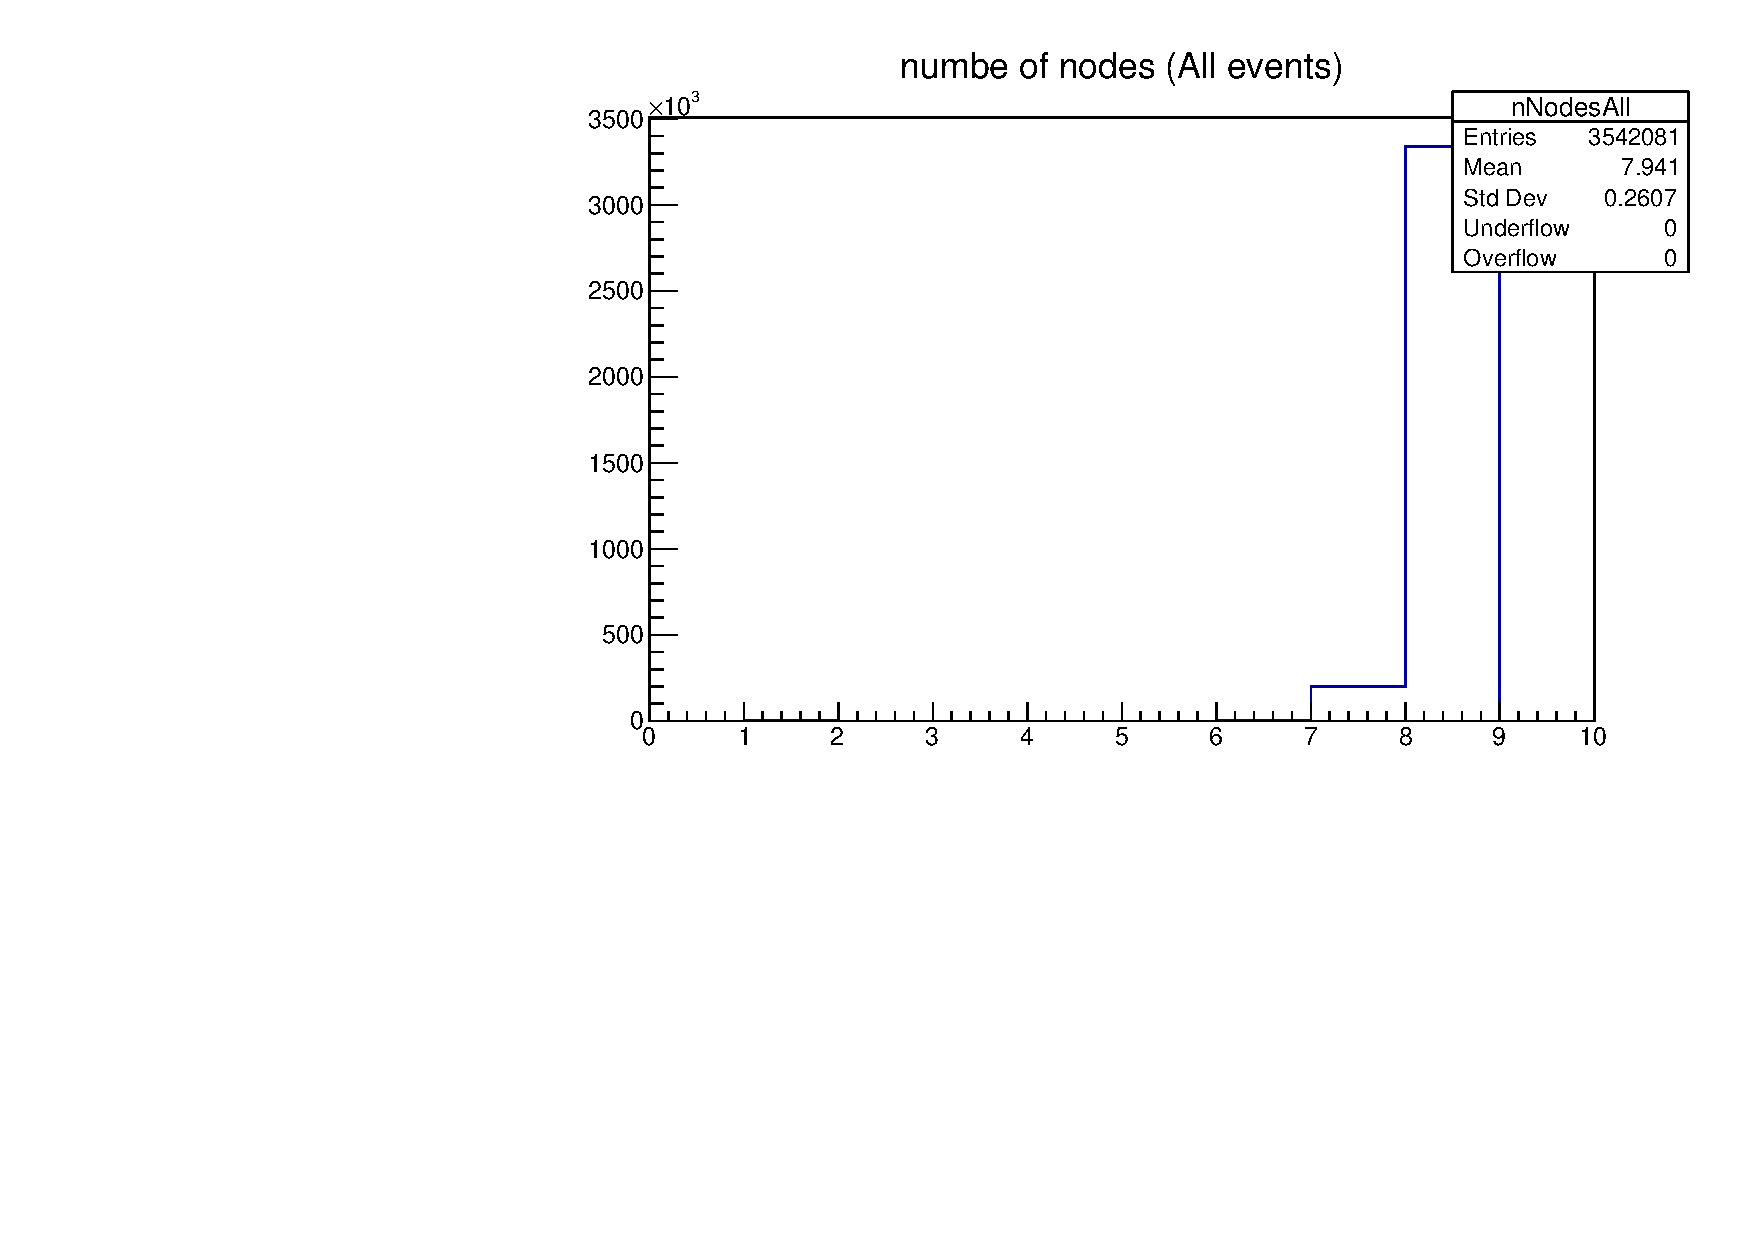
\includegraphics[width=0.33\textwidth,scale=0.5,trim=0 0 0 0,clip]{plotsdir/file0_test-nNodesAll-1.pdf} 
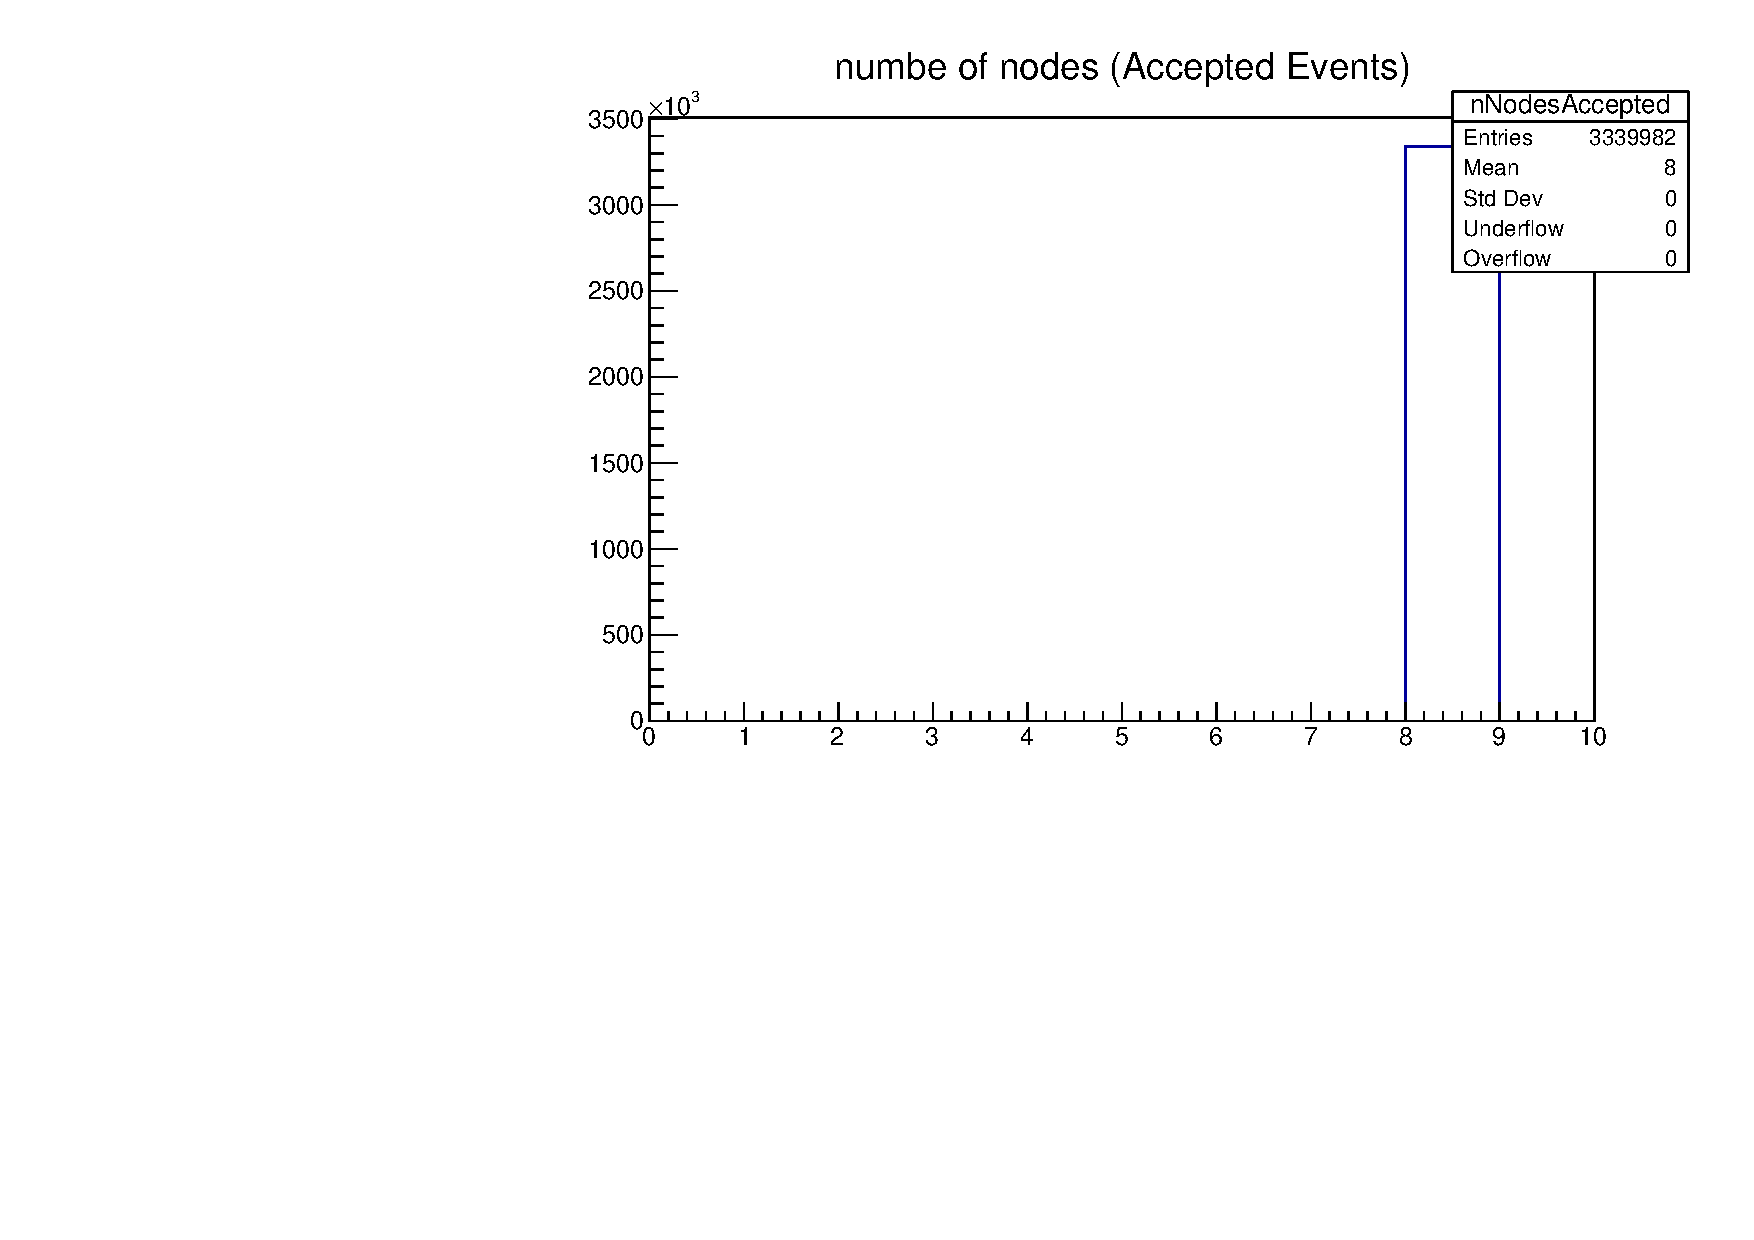
\includegraphics[width=0.33\textwidth,scale=0.5,trim=0 0 0 0,clip]{plotsdir/file0_test-nNodesAccepted-1.pdf} 
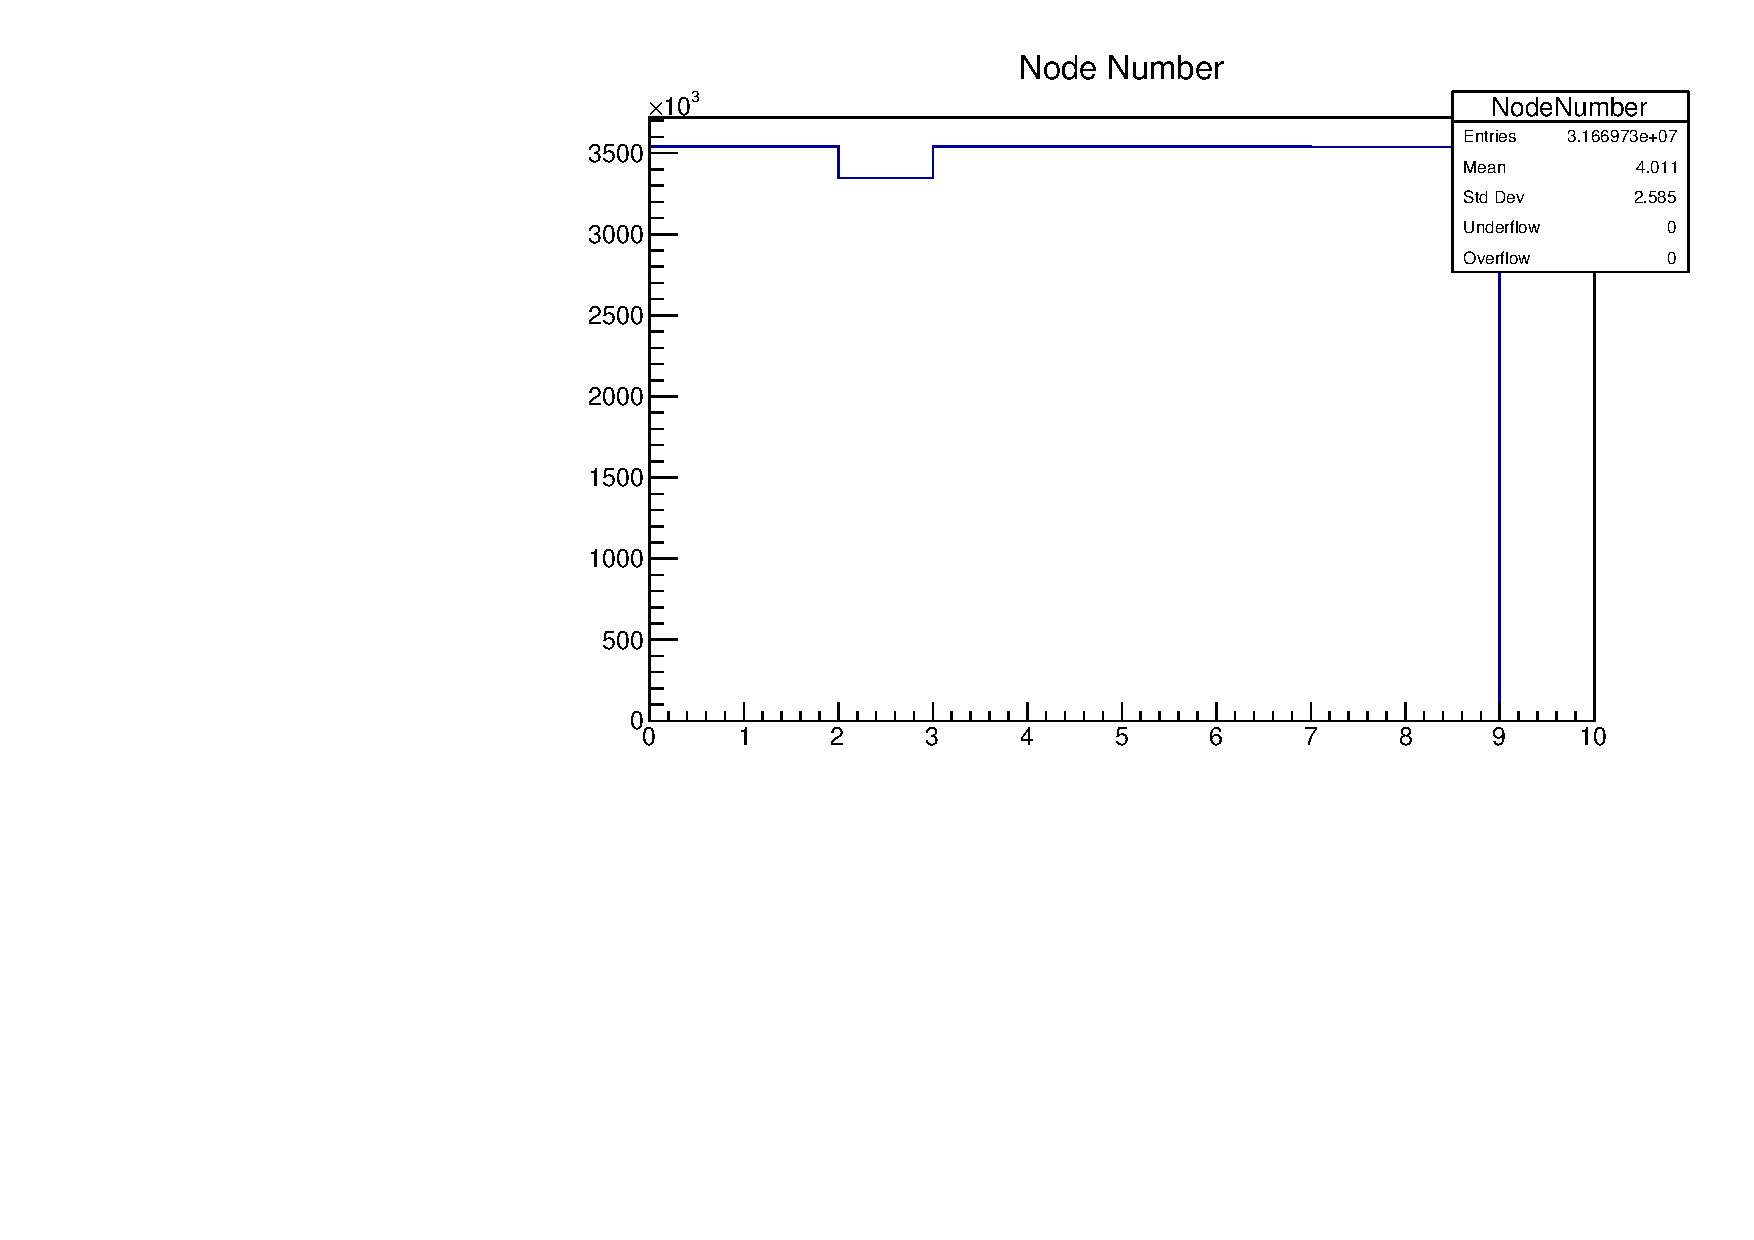
\includegraphics[width=0.33\textwidth,scale=0.5,trim=0 0 0 0,clip]{plotsdir/file0_test-NodeNumber-1.pdf} 
\caption{(a)numbe of nodes (All events) ~~~(b) numbe of nodes (Accepted Events) ~~~(c)Node Number } 
\end{figure} 
\begin{figure}[H] 
\vspace*{-0.3cm} 
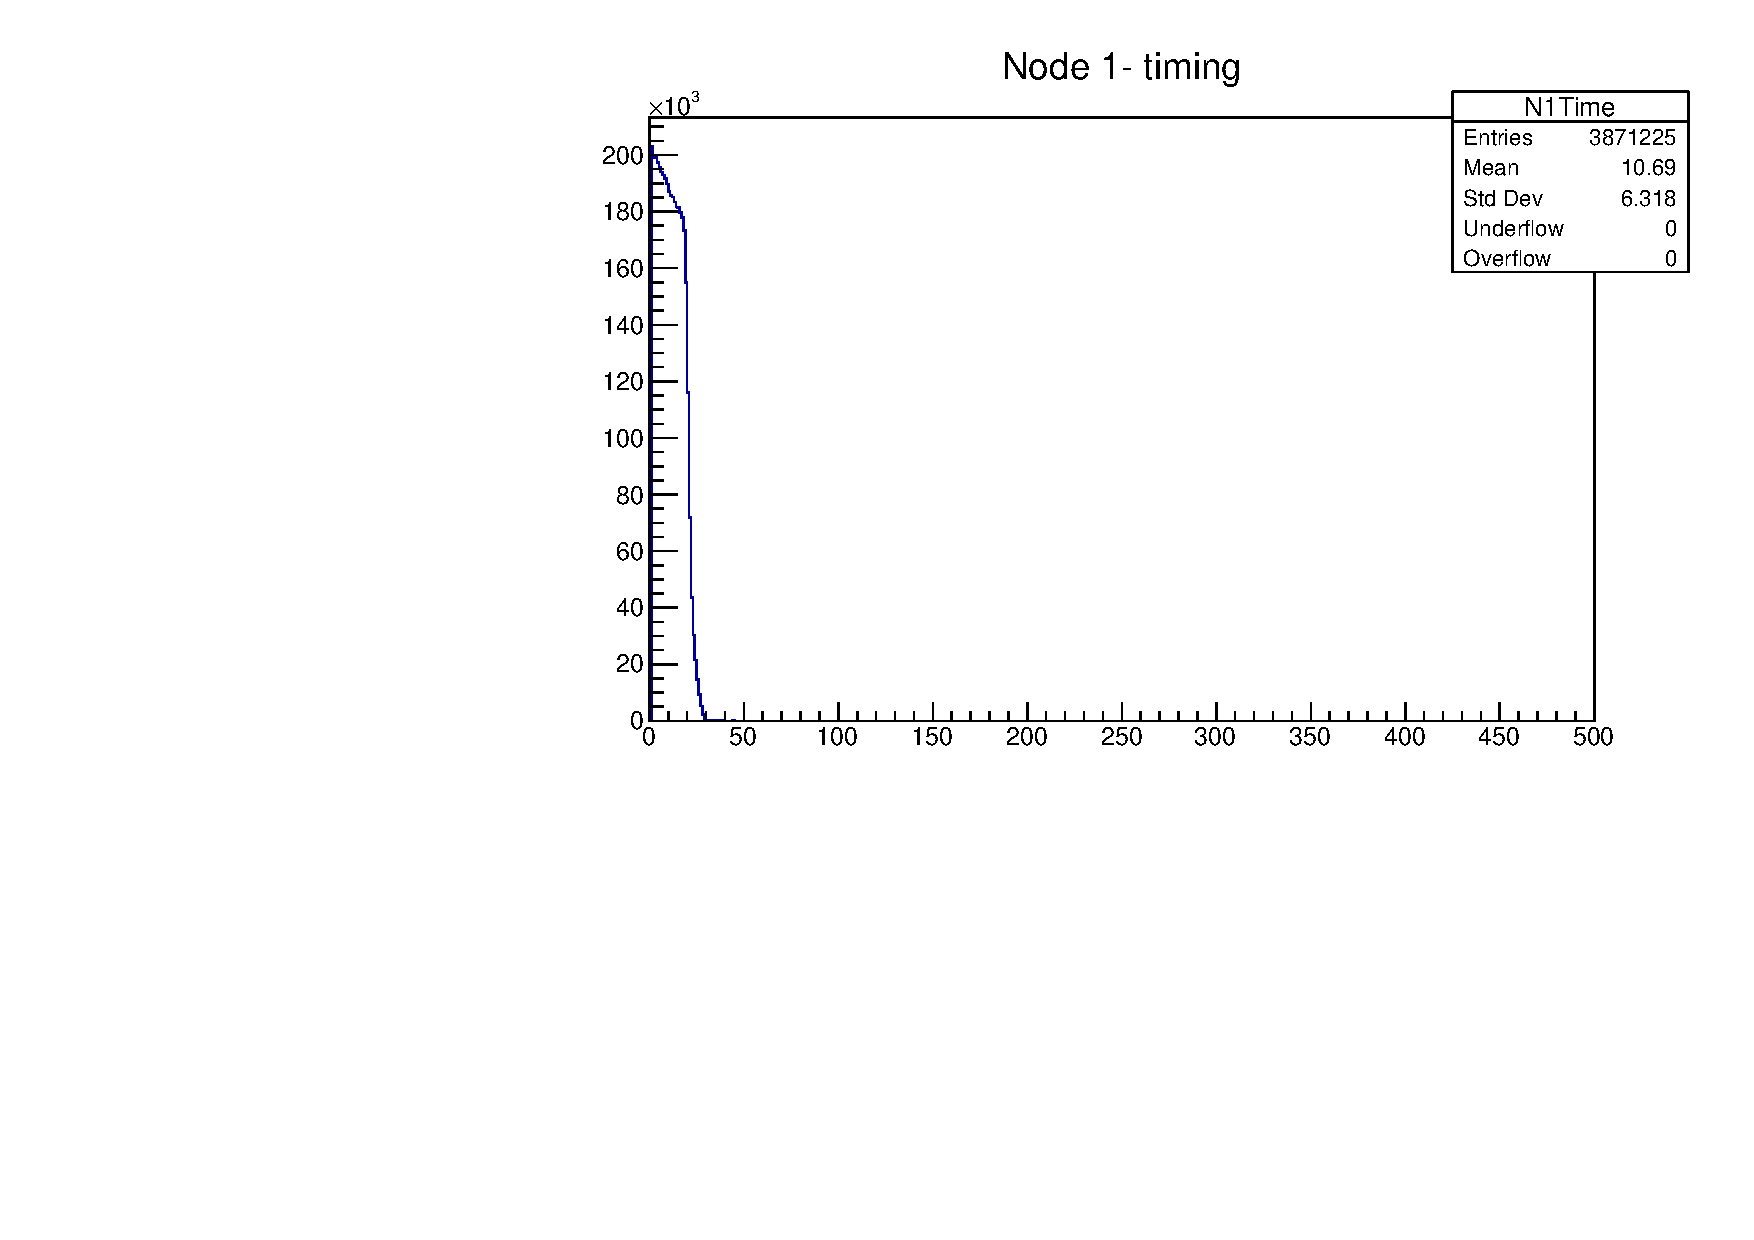
\includegraphics[width=0.33\textwidth,scale=0.5,trim=0 0 0 0,clip]{plotsdir/file0_test-N1Time-1.pdf} 
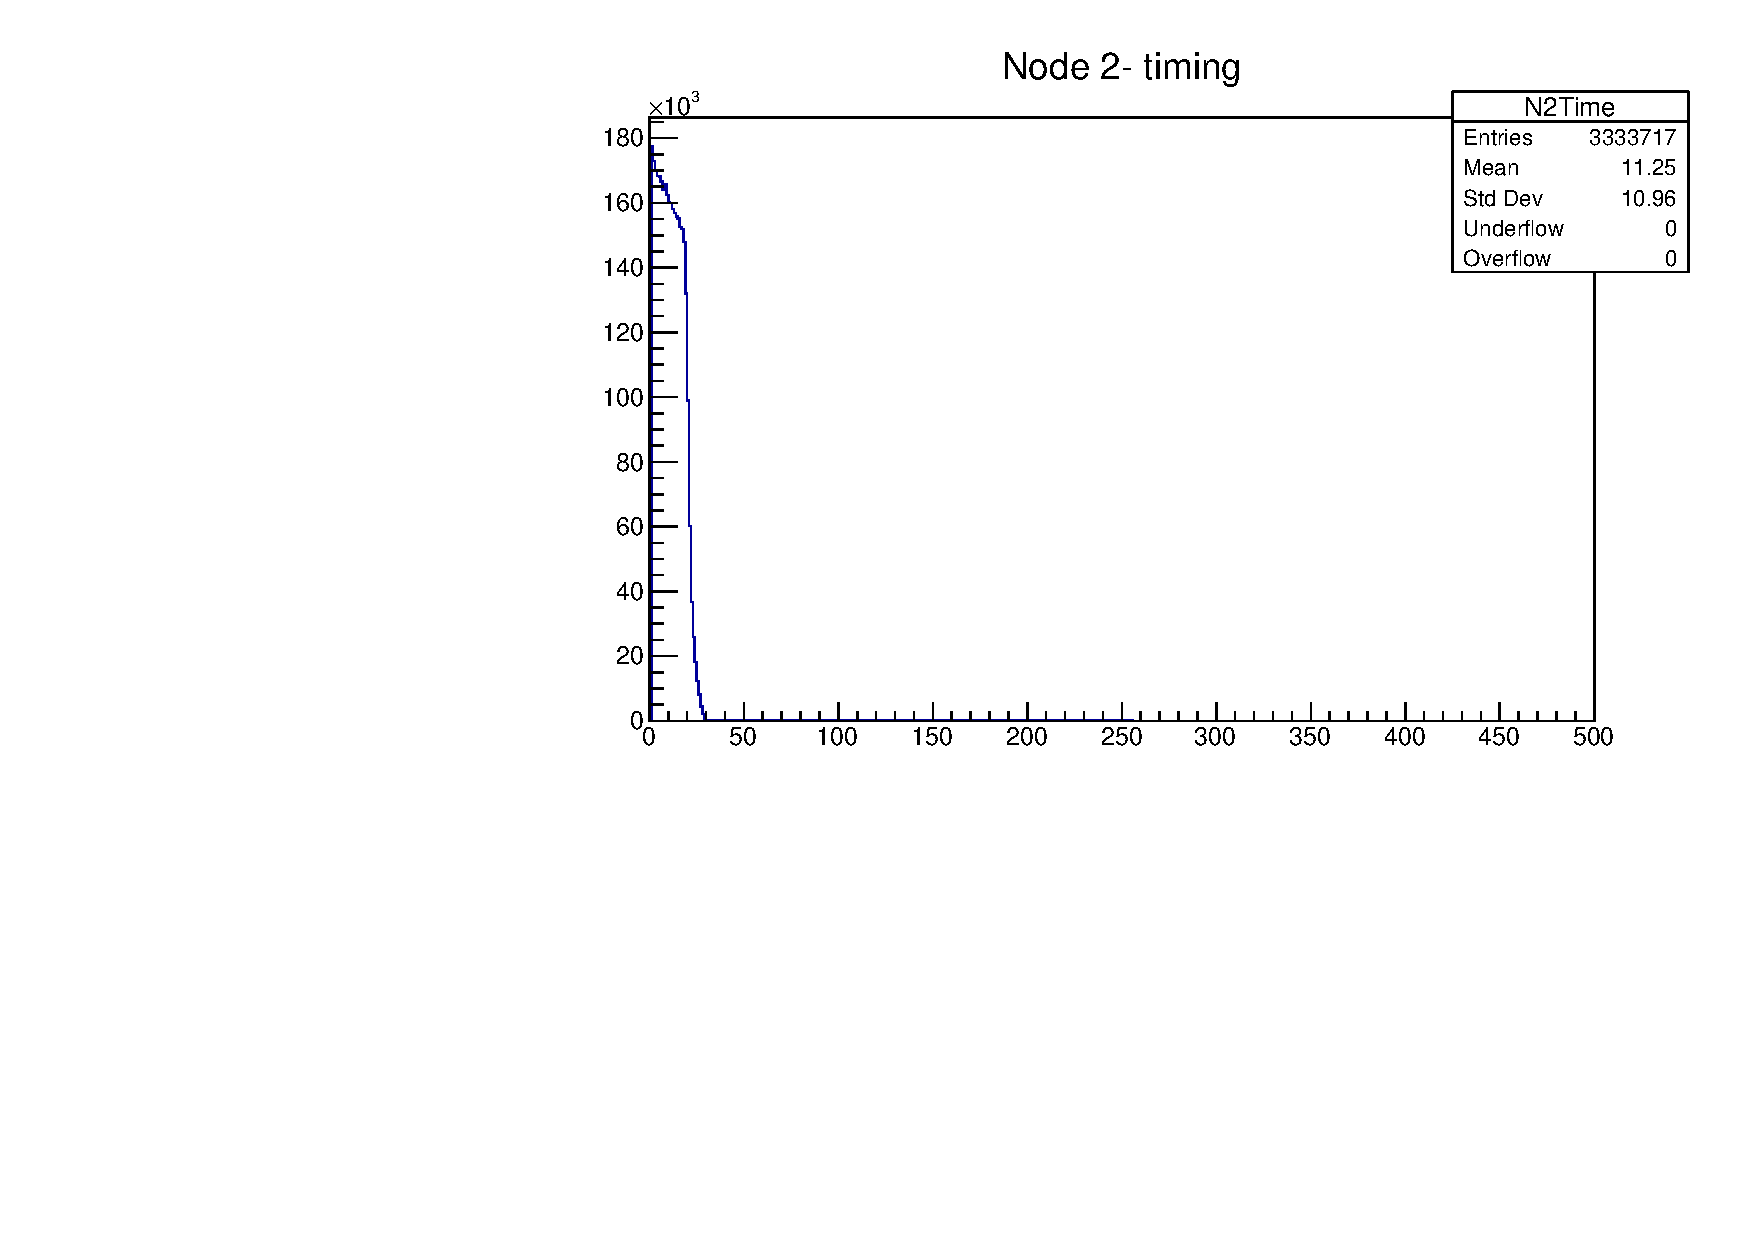
\includegraphics[width=0.33\textwidth,scale=0.5,trim=0 0 0 0,clip]{plotsdir/file0_test-N2Time-1.pdf} 
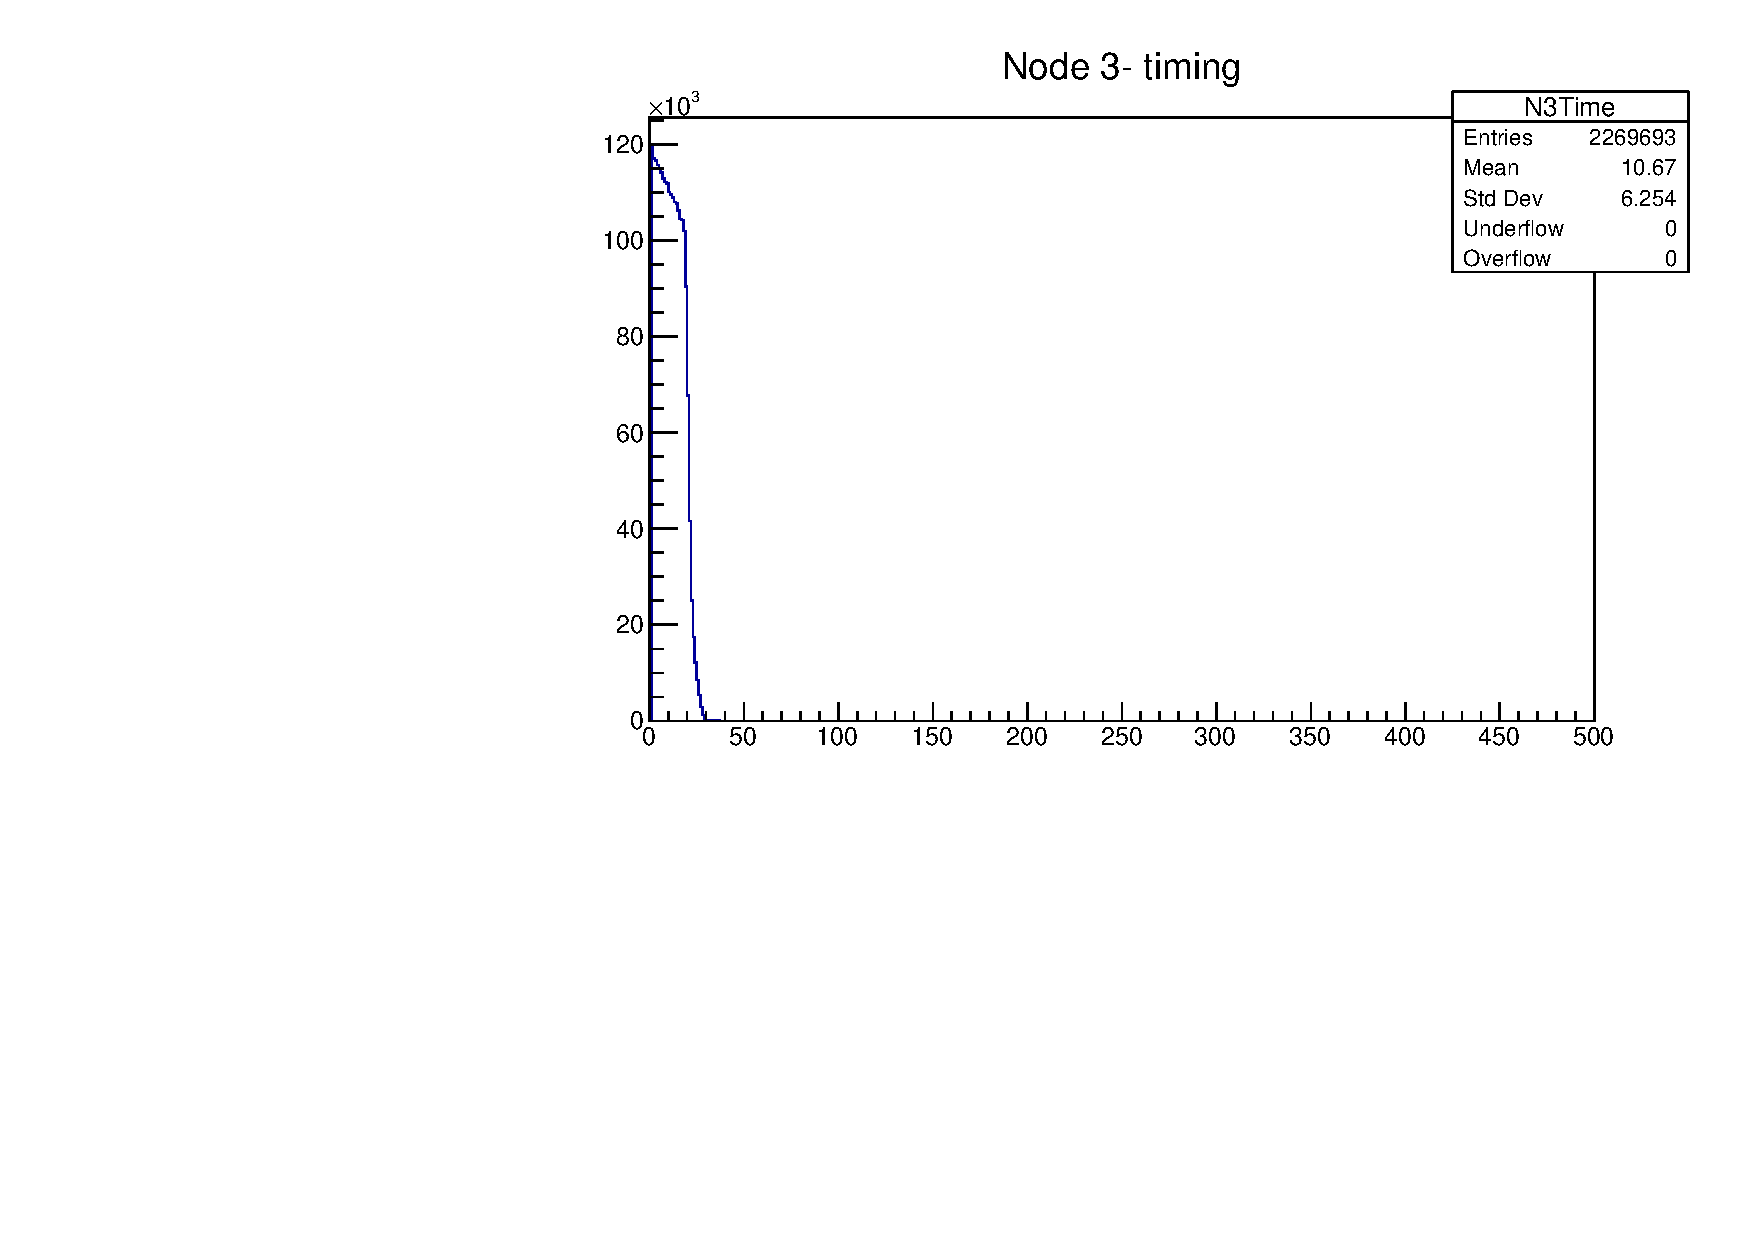
\includegraphics[width=0.33\textwidth,scale=0.5,trim=0 0 0 0,clip]{plotsdir/file0_test-N3Time-1.pdf} 
\caption{(a)Node 1- timing ~~~(b) Node 2- timing ~~~(c)Node 3- timing } 
\end{figure} 
\begin{figure}[H] 
\vspace*{-0.3cm} 
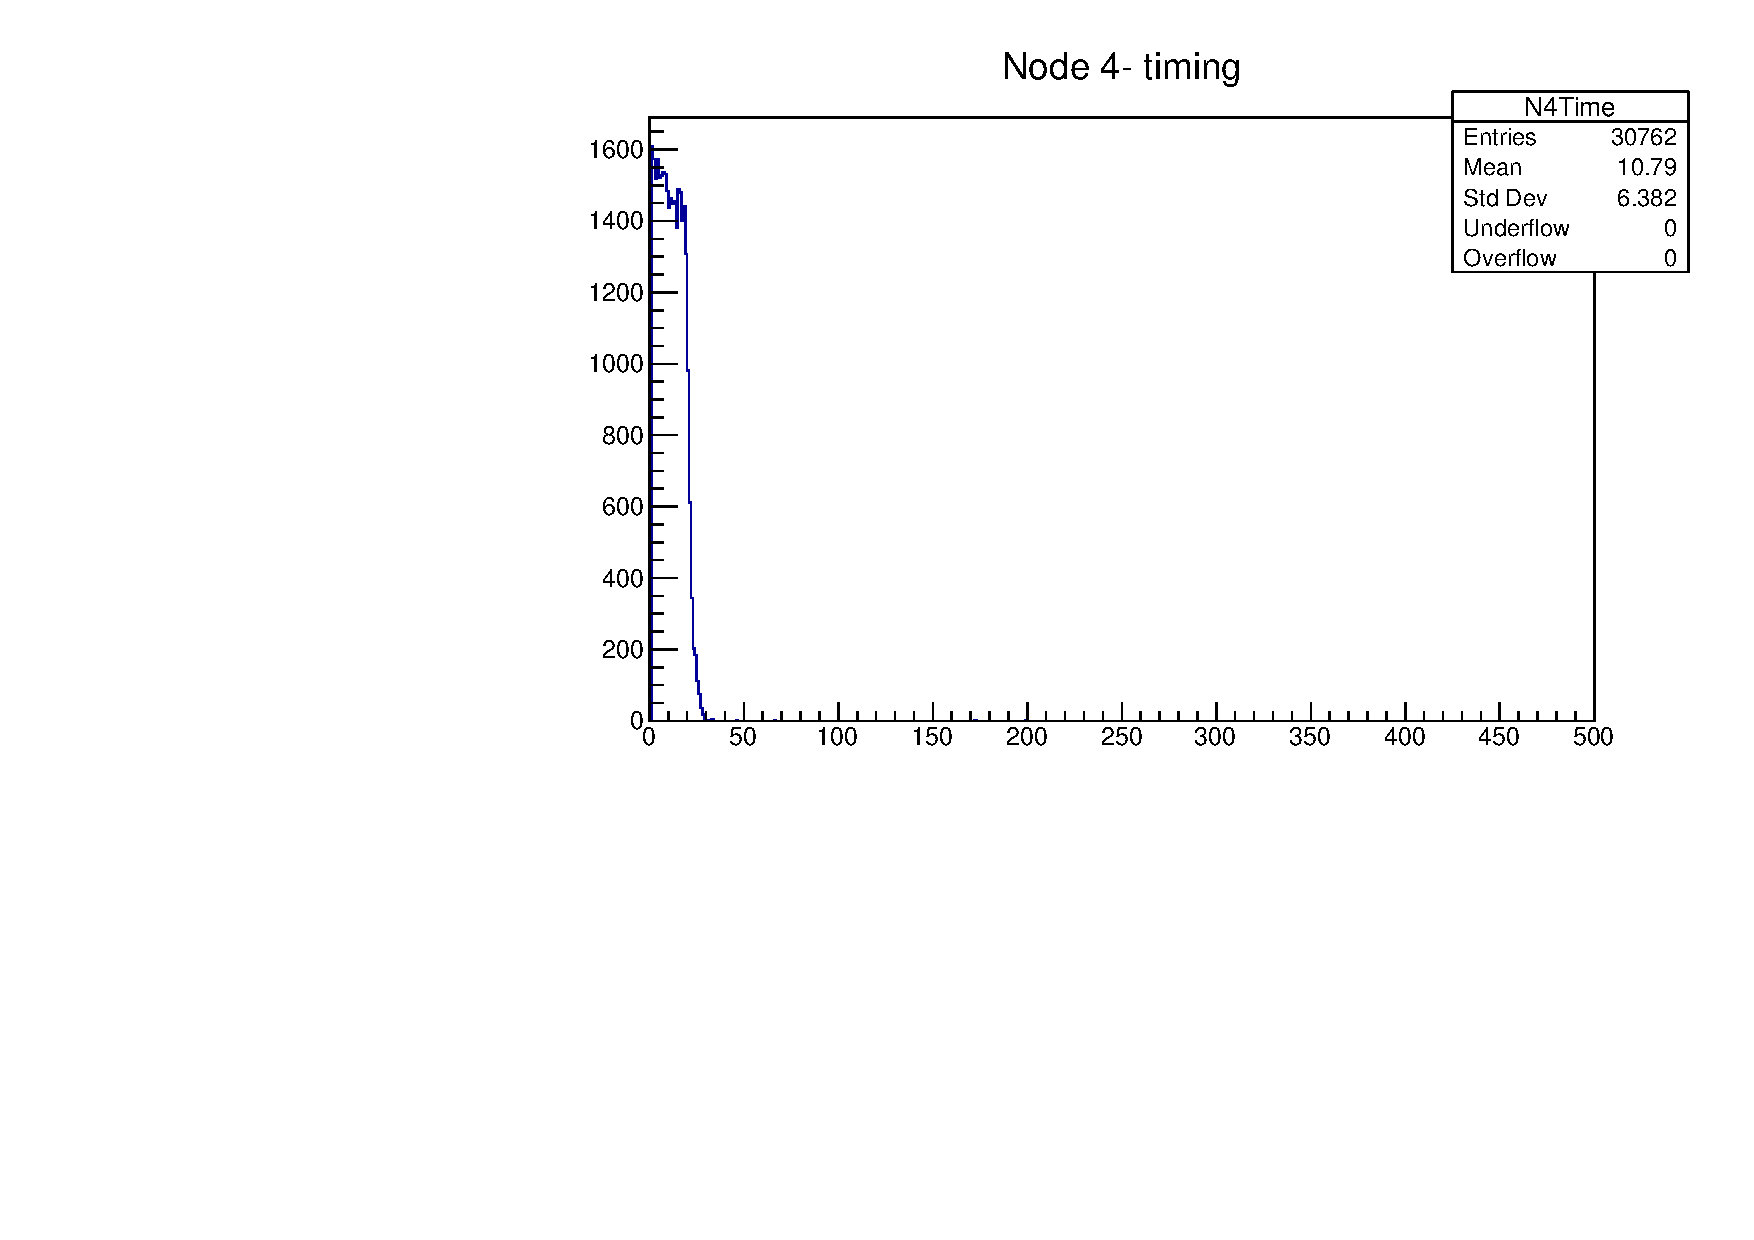
\includegraphics[width=0.33\textwidth,scale=0.5,trim=0 0 0 0,clip]{plotsdir/file0_test-N4Time-1.pdf} 
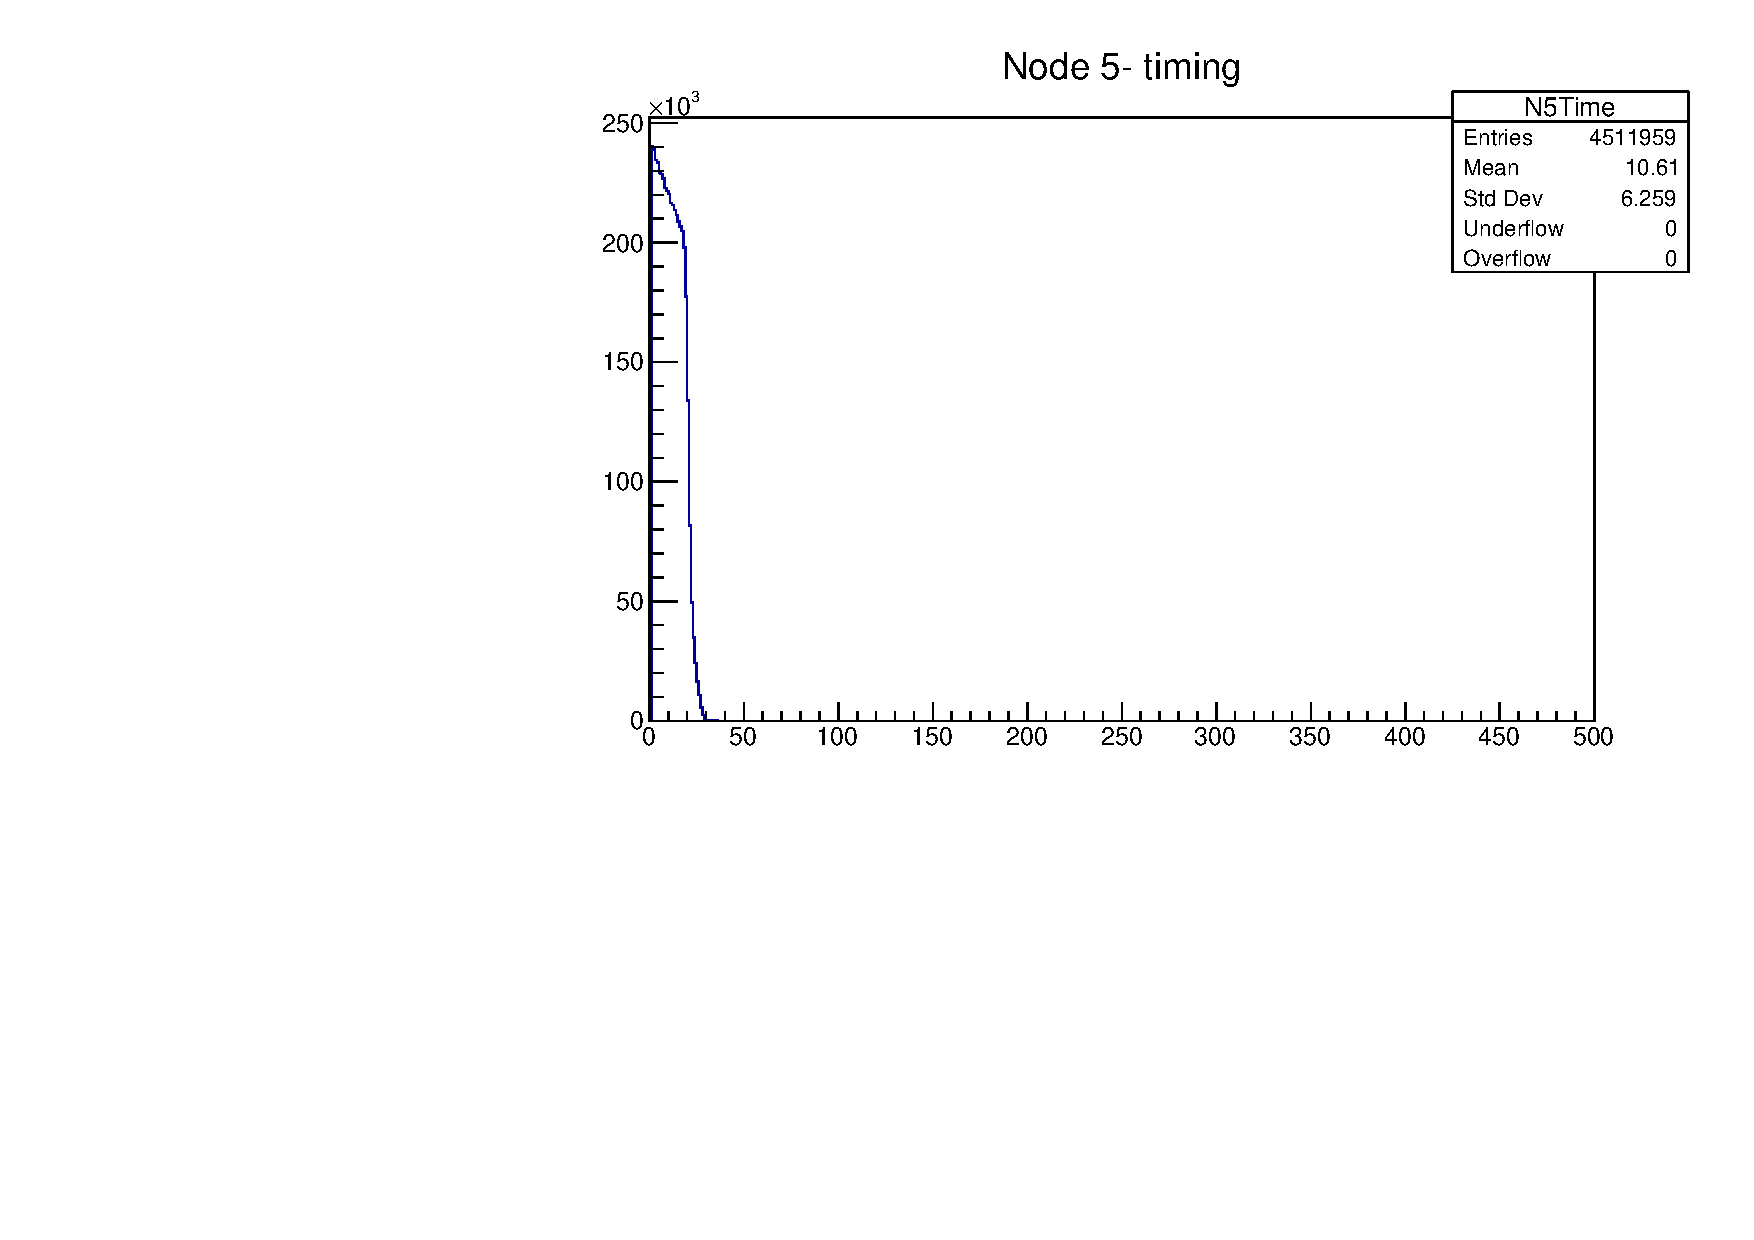
\includegraphics[width=0.33\textwidth,scale=0.5,trim=0 0 0 0,clip]{plotsdir/file0_test-N5Time-1.pdf} 
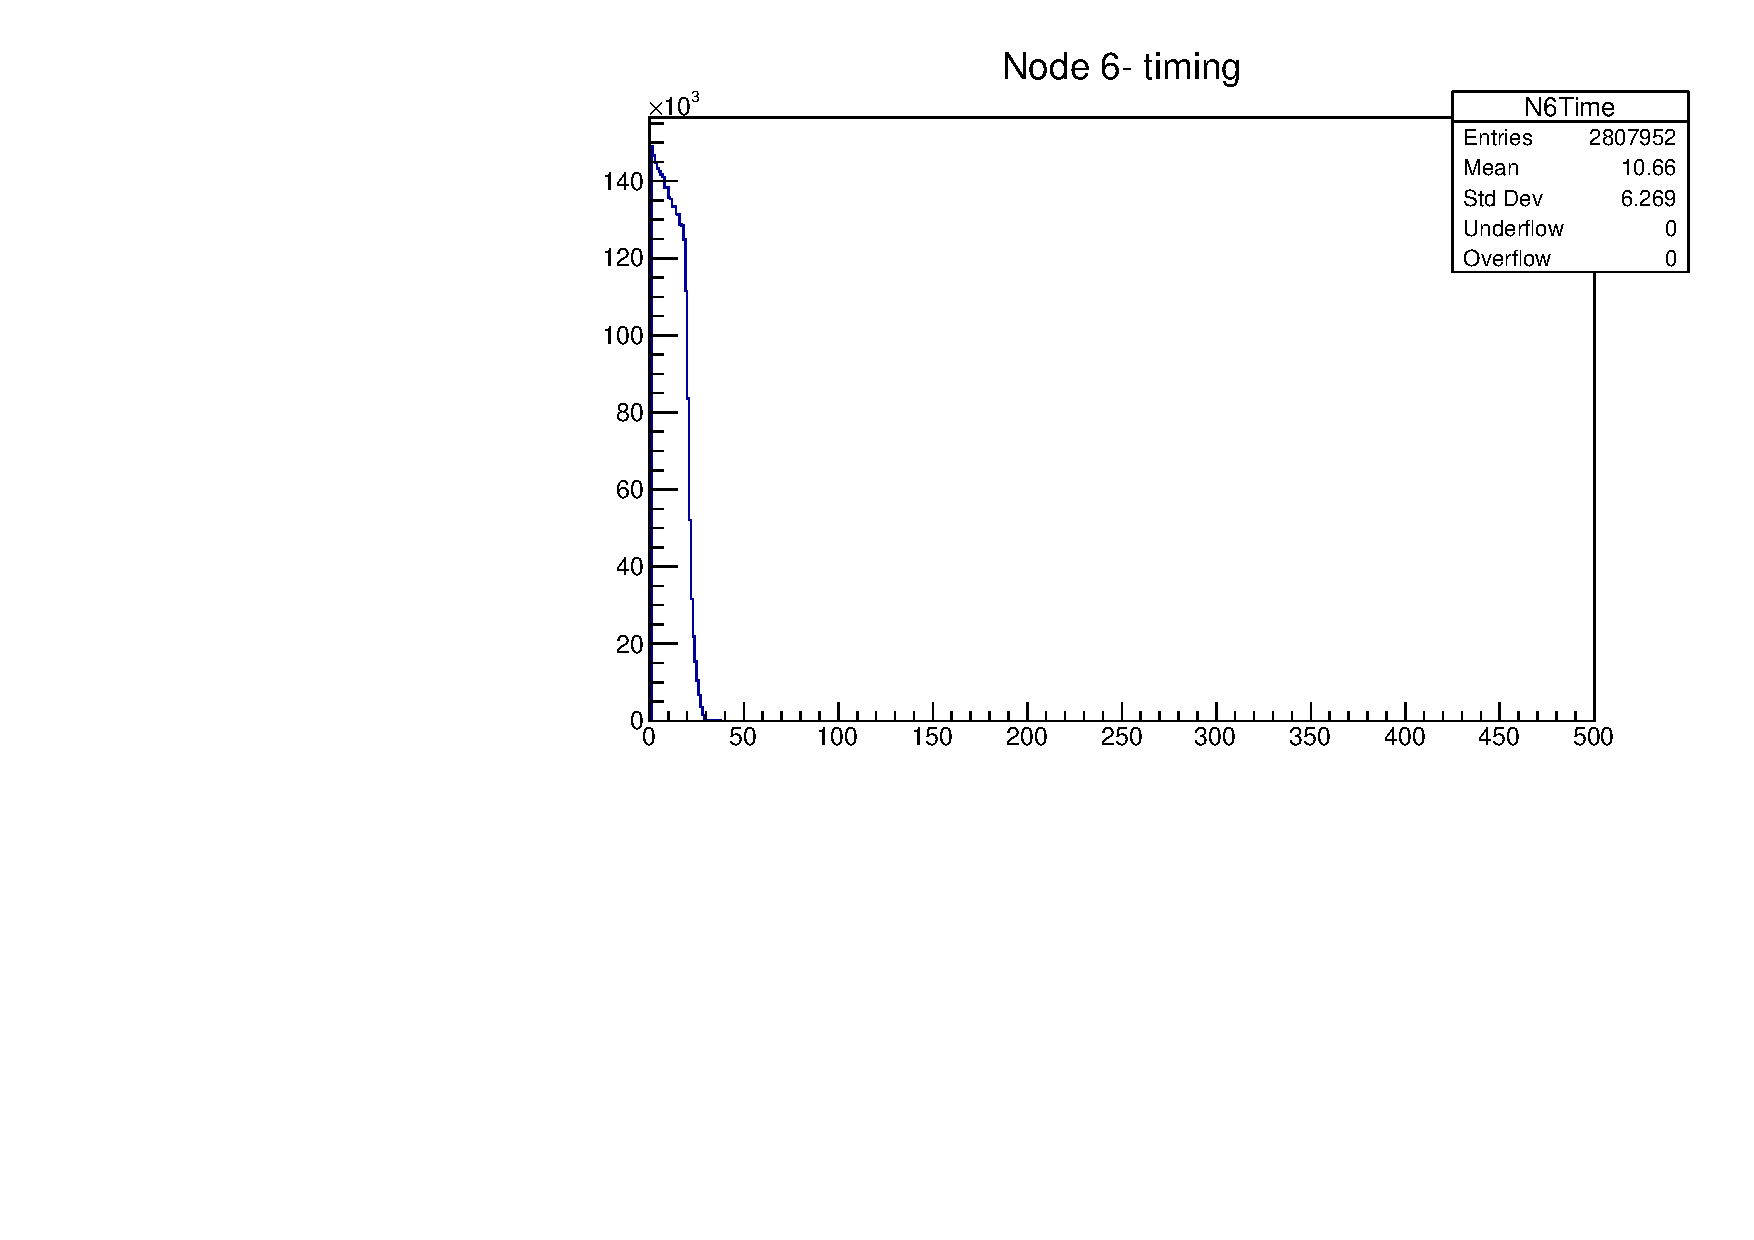
\includegraphics[width=0.33\textwidth,scale=0.5,trim=0 0 0 0,clip]{plotsdir/file0_test-N6Time-1.pdf} 
\caption{(a)Node 4- timing ~~~(b) Node 5- timing ~~~(c)Node 6- timing } 
\end{figure} 
\begin{figure}[H] 
\vspace*{-0.3cm} 
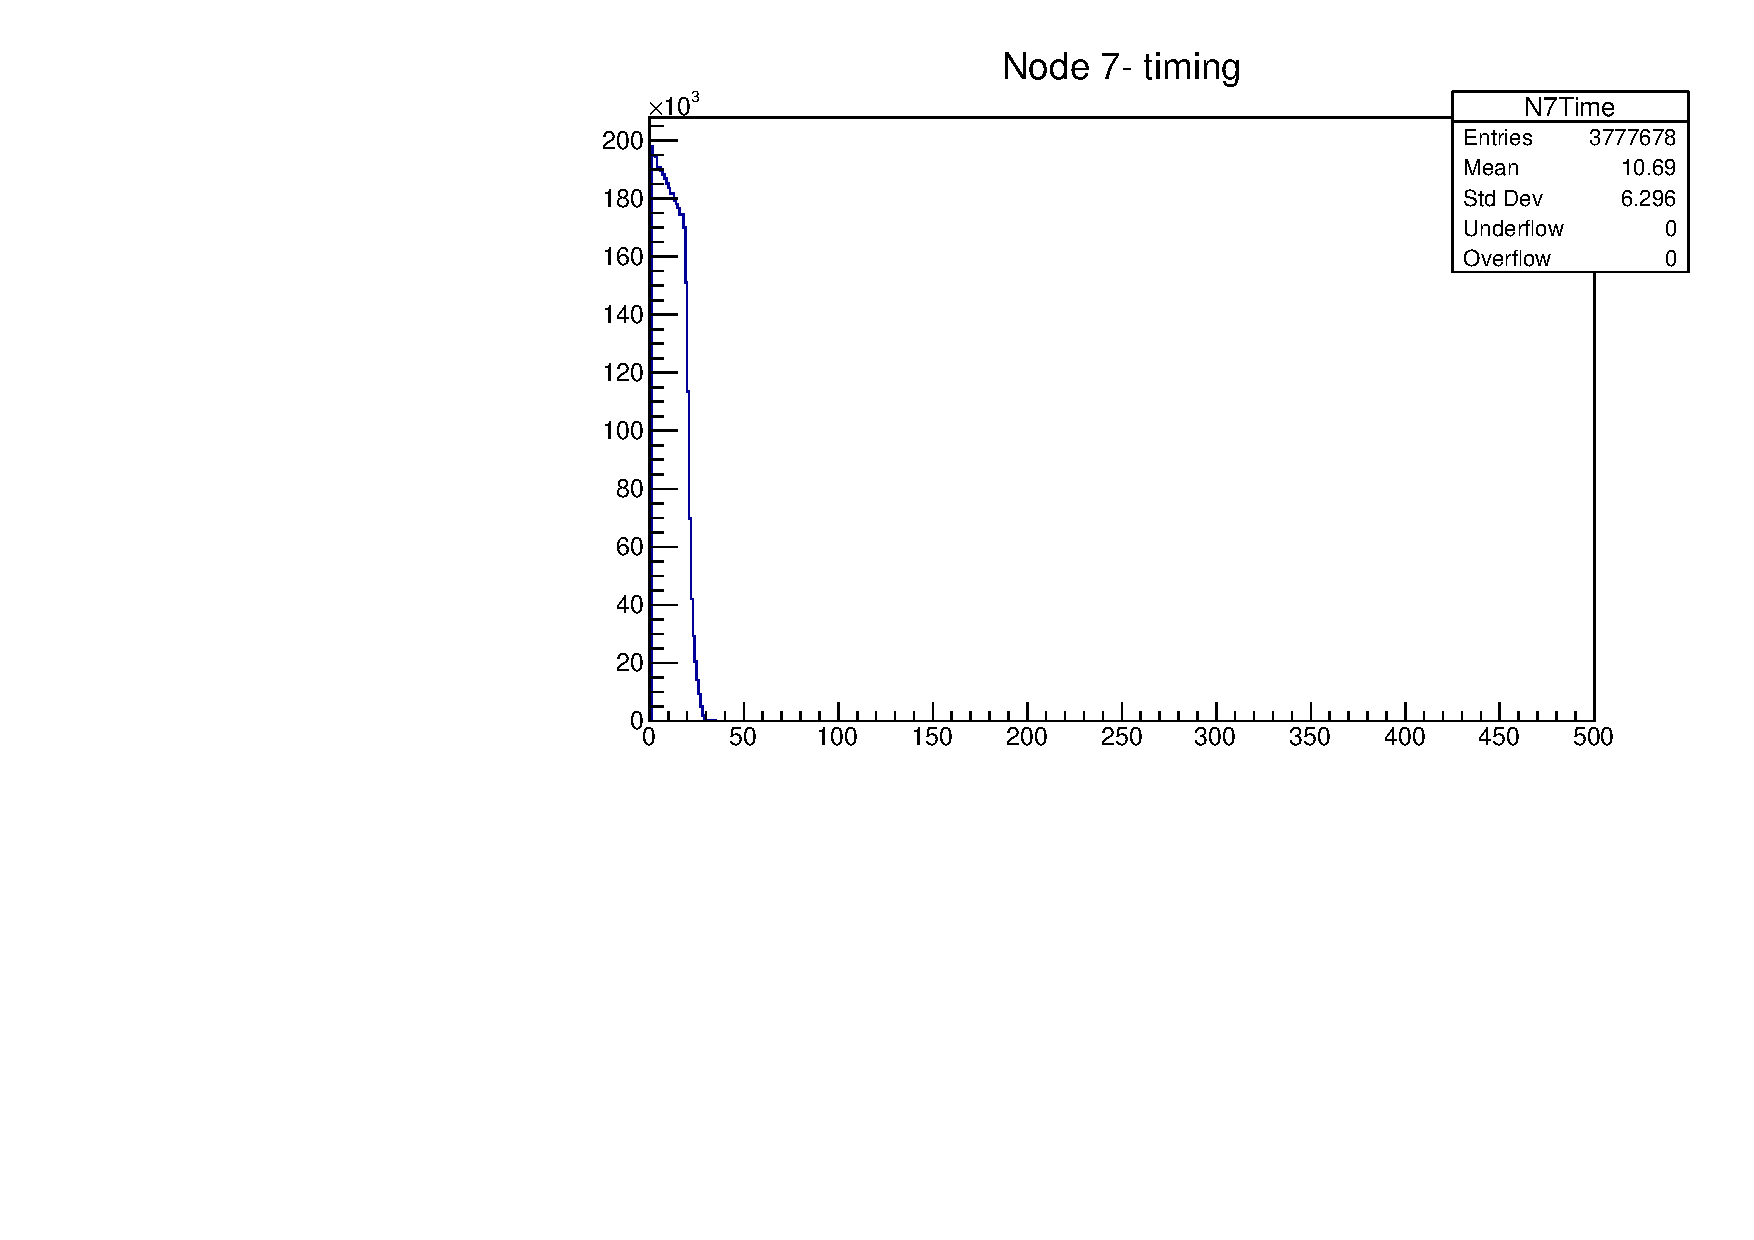
\includegraphics[width=0.33\textwidth,scale=0.5,trim=0 0 0 0,clip]{plotsdir/file0_test-N7Time-1.pdf} 
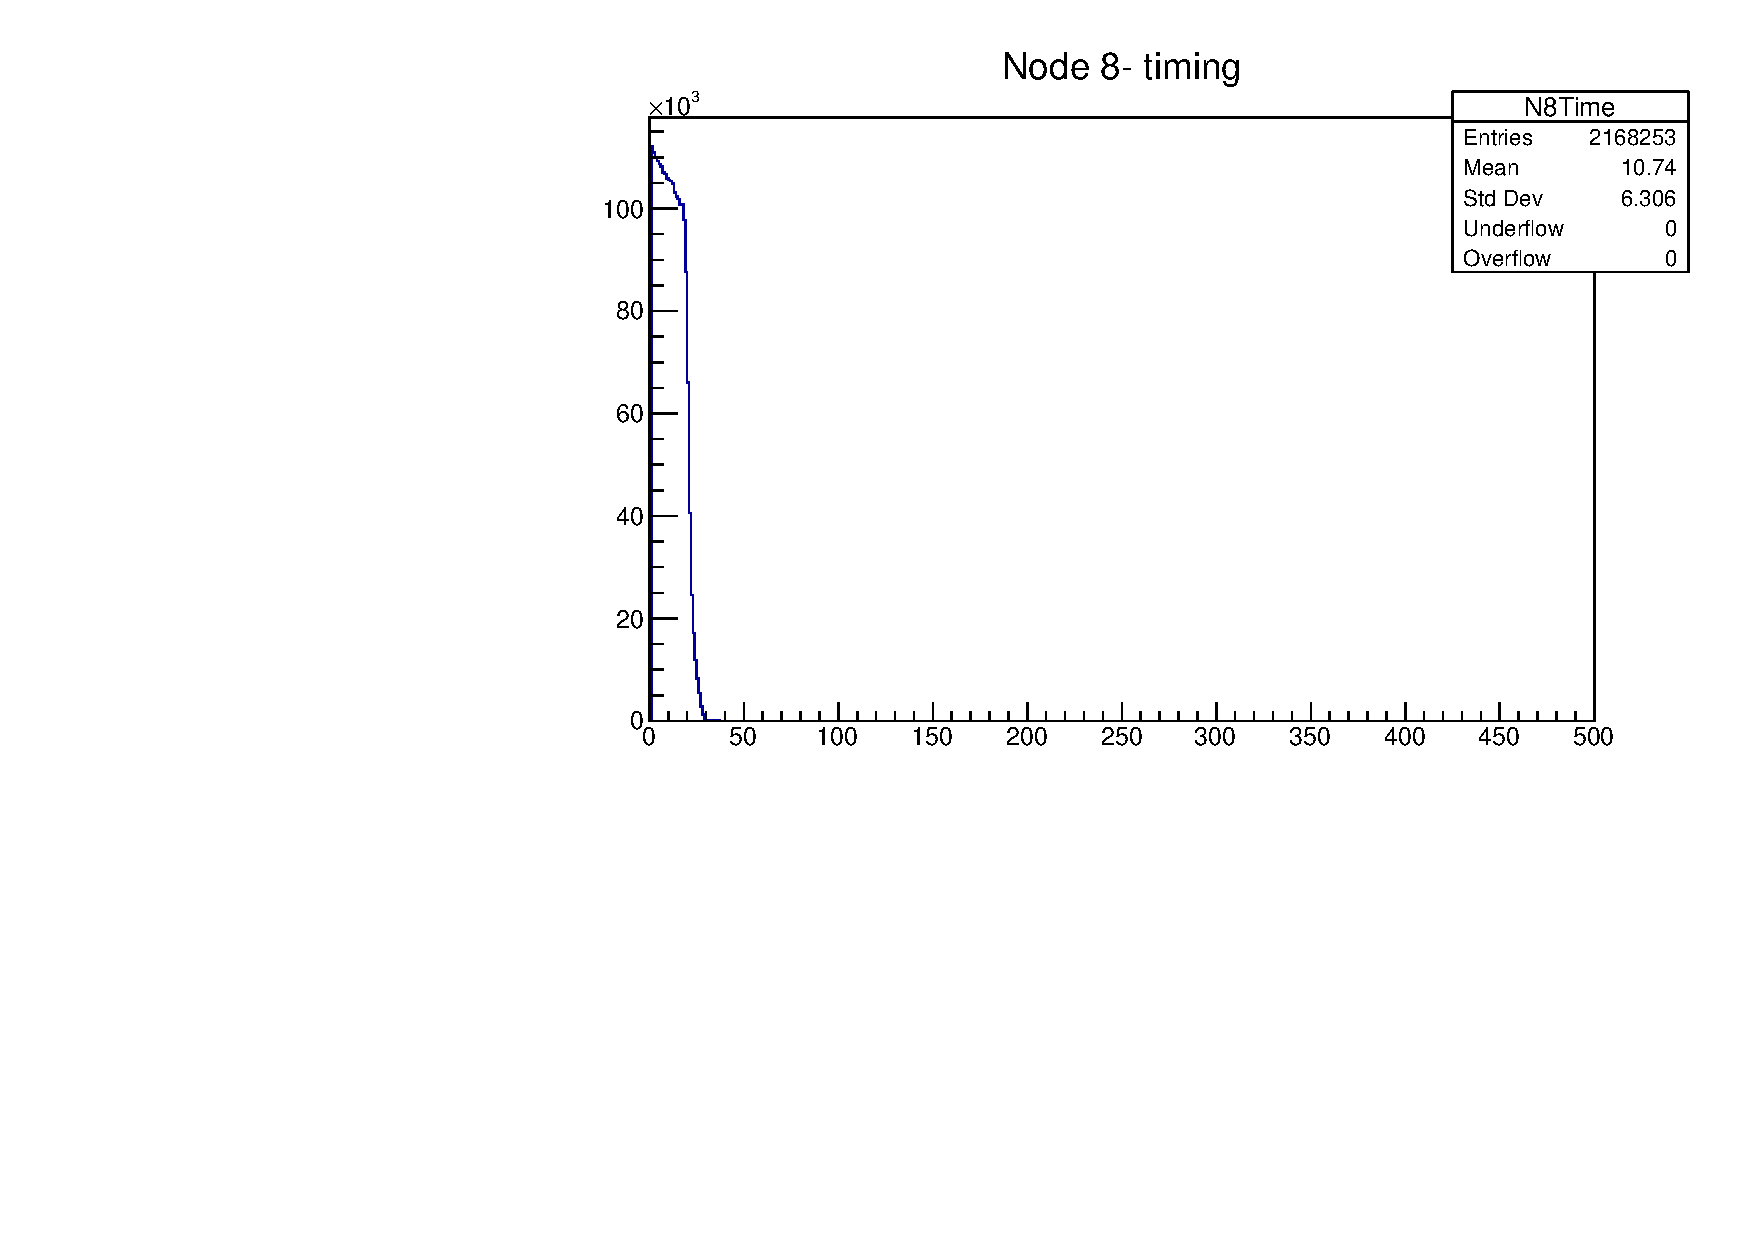
\includegraphics[width=0.33\textwidth,scale=0.5,trim=0 0 0 0,clip]{plotsdir/file0_test-N8Time-1.pdf} 
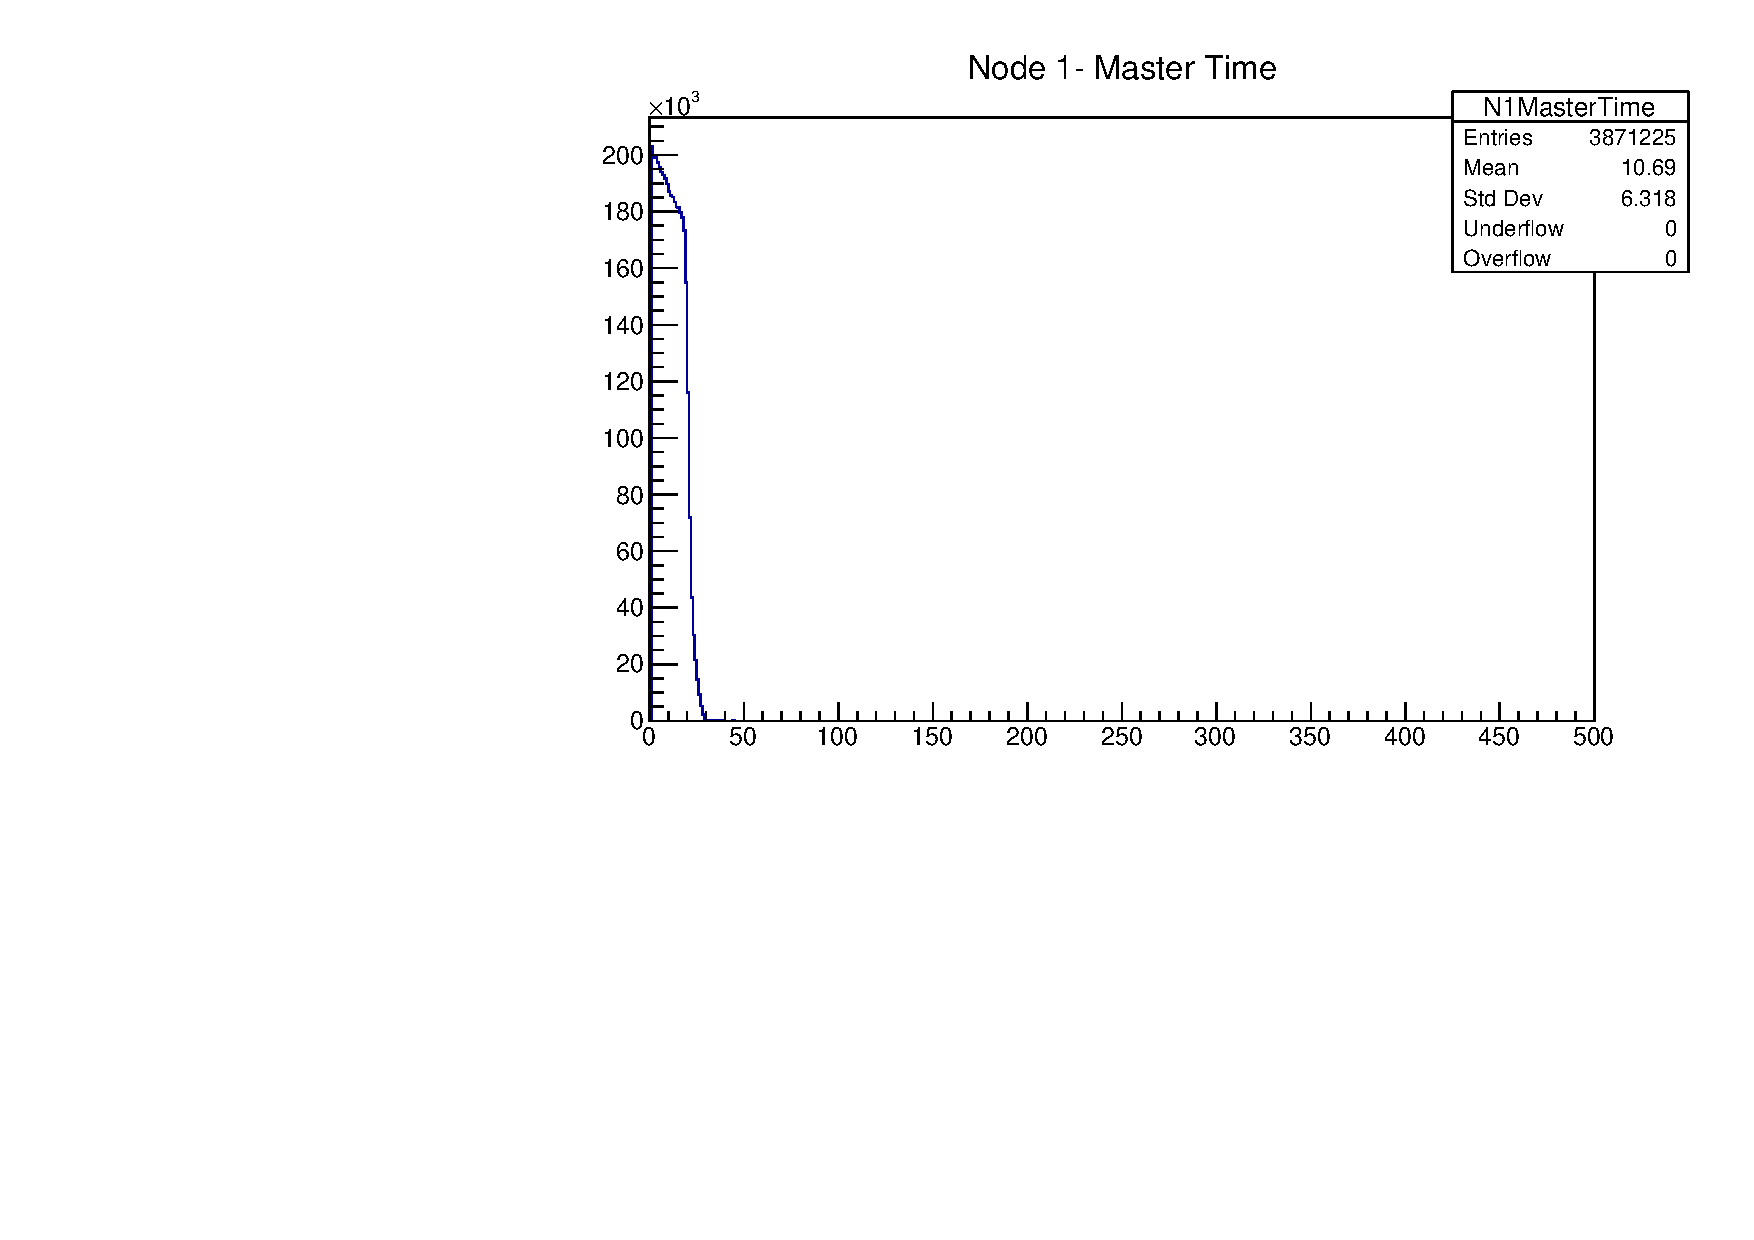
\includegraphics[width=0.33\textwidth,scale=0.5,trim=0 0 0 0,clip]{plotsdir/file0_test-N1MasterTime-1.pdf} 
\caption{(a)Node 7- timing ~~~(b) Node 8- timing ~~~(c)Node 1- Master Time } 
\end{figure} 
\begin{figure}[H] 
\vspace*{-0.3cm} 
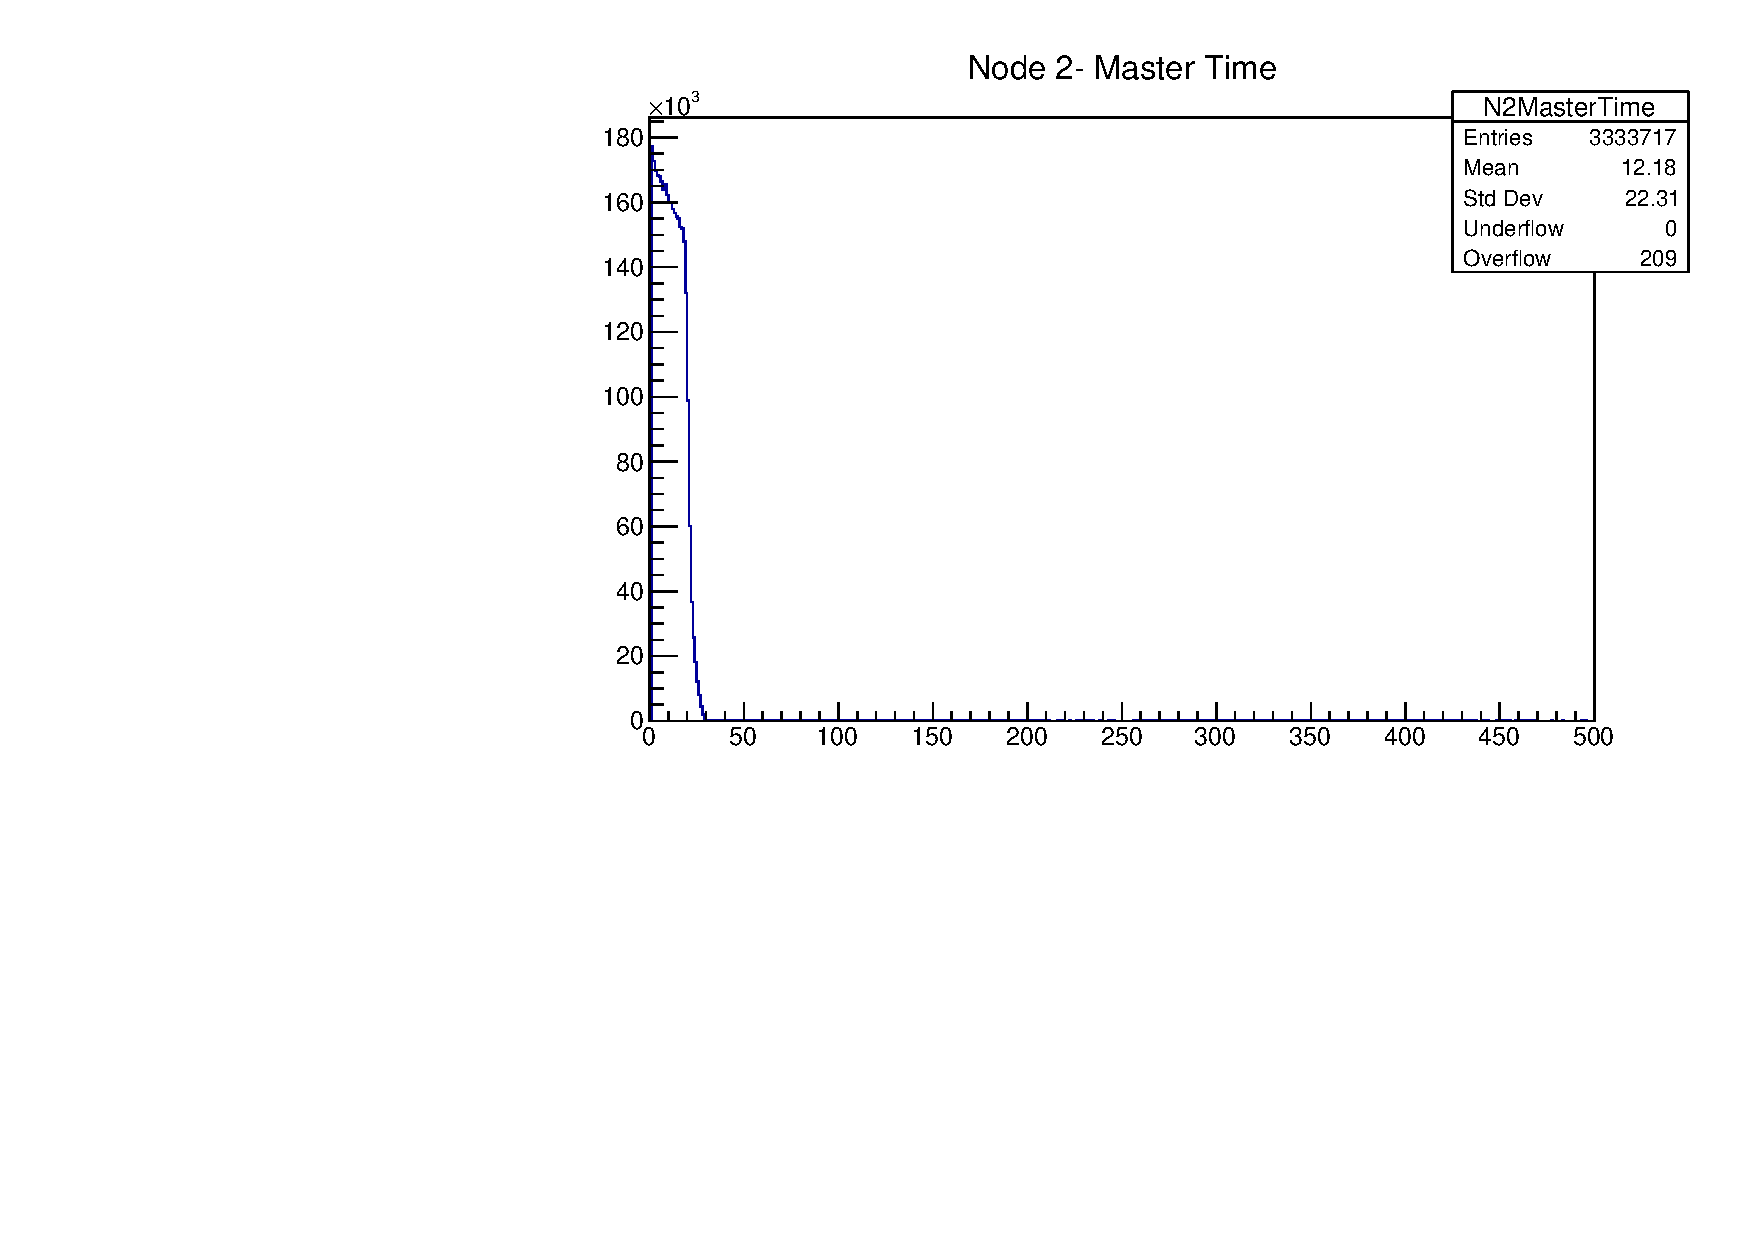
\includegraphics[width=0.33\textwidth,scale=0.5,trim=0 0 0 0,clip]{plotsdir/file0_test-N2MasterTime-1.pdf} 
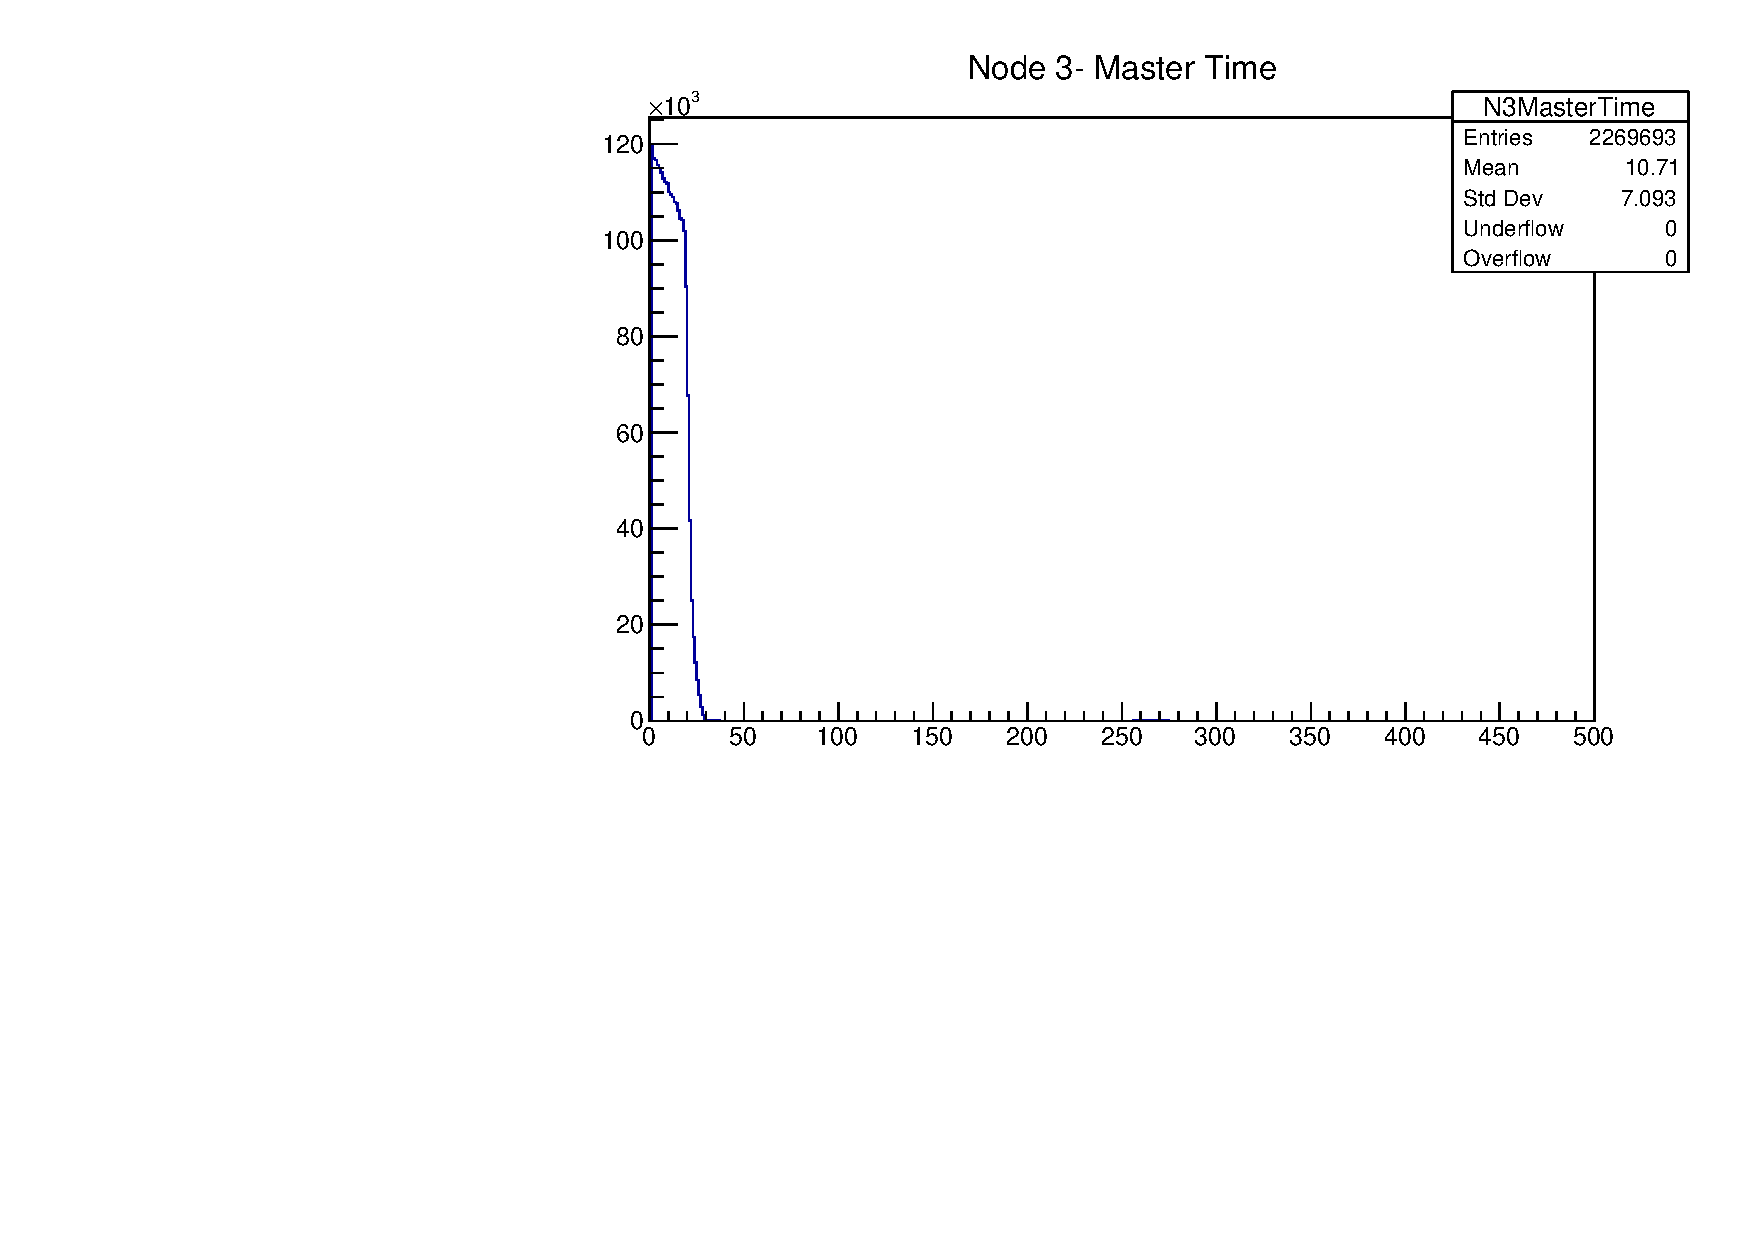
\includegraphics[width=0.33\textwidth,scale=0.5,trim=0 0 0 0,clip]{plotsdir/file0_test-N3MasterTime-1.pdf} 
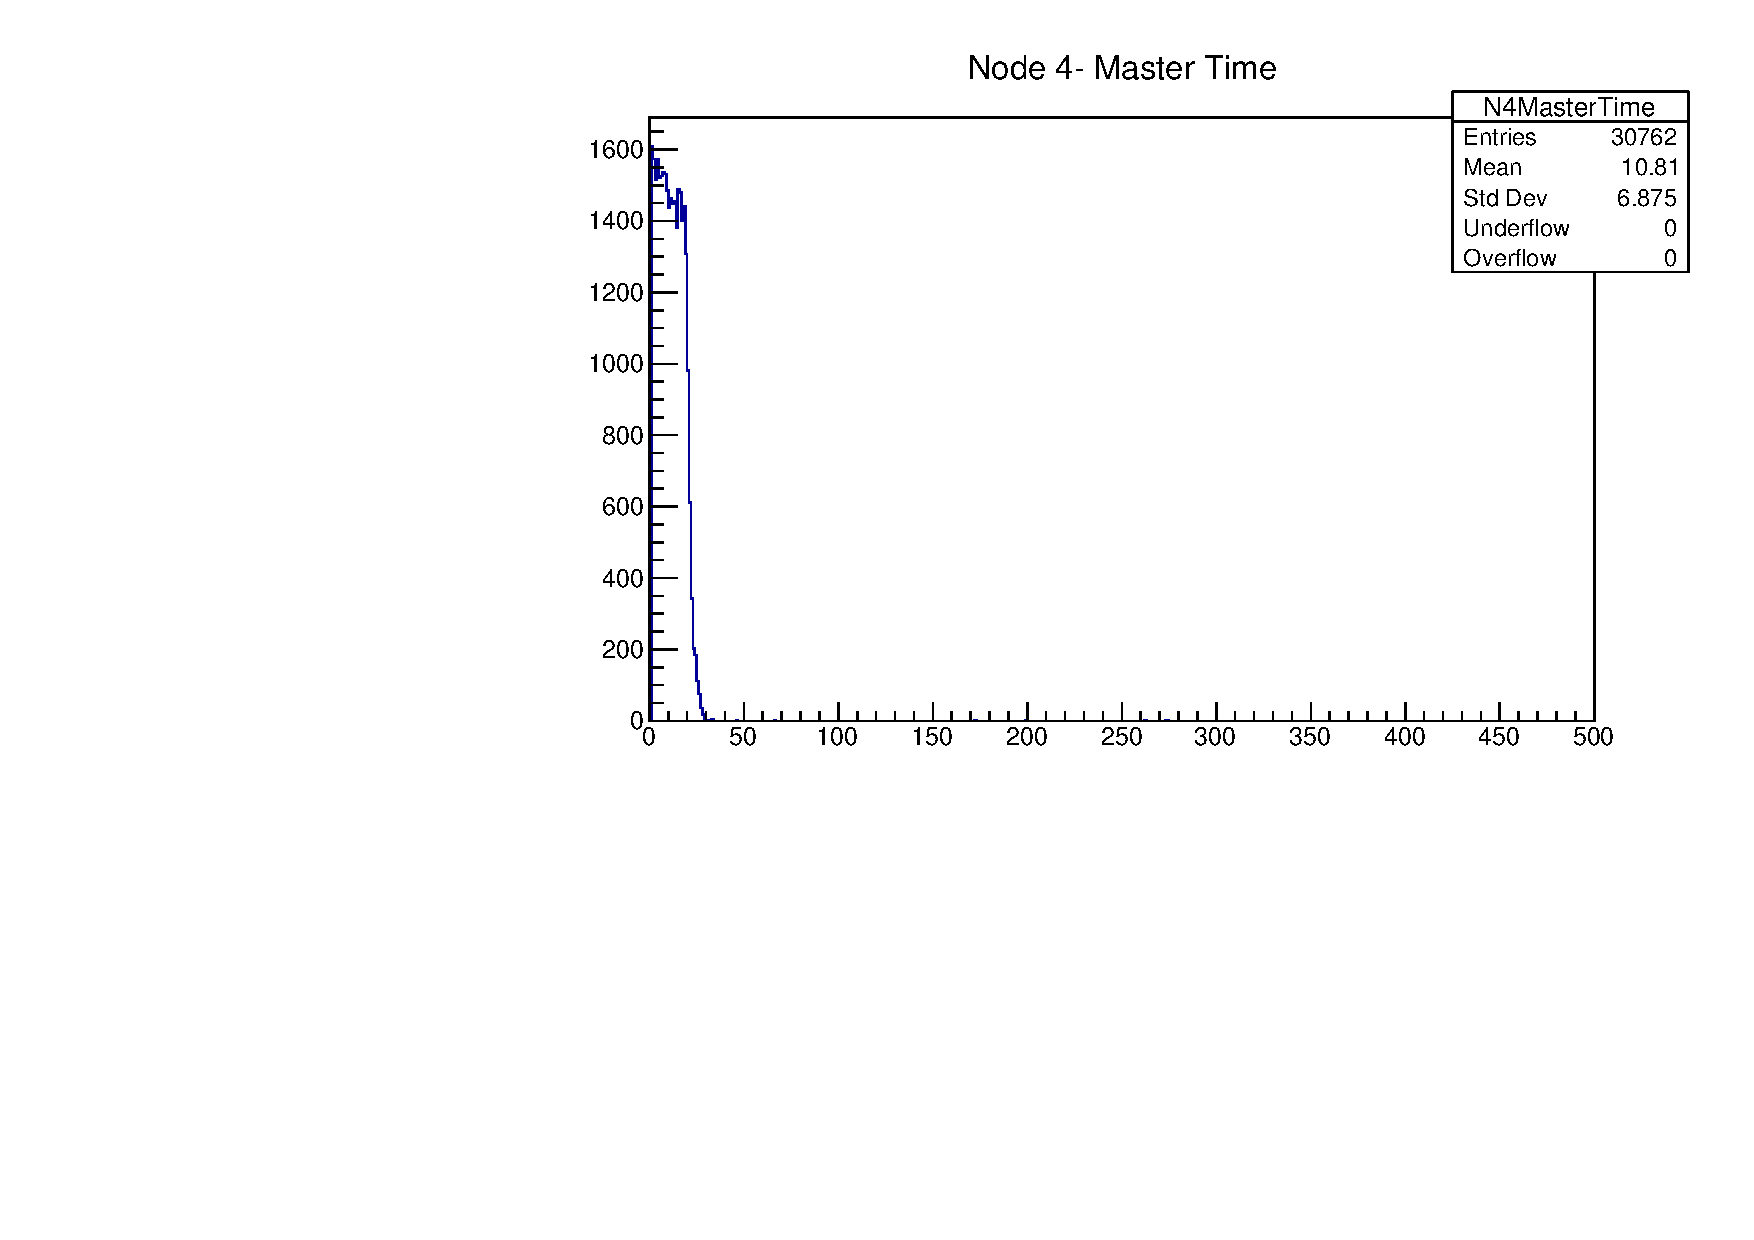
\includegraphics[width=0.33\textwidth,scale=0.5,trim=0 0 0 0,clip]{plotsdir/file0_test-N4MasterTime-1.pdf} 
\caption{(a)Node 2- Master Time ~~~(b) Node 3- Master Time ~~~(c)Node 4- Master Time } 
\end{figure} 
\begin{figure}[H] 
\vspace*{-0.3cm} 
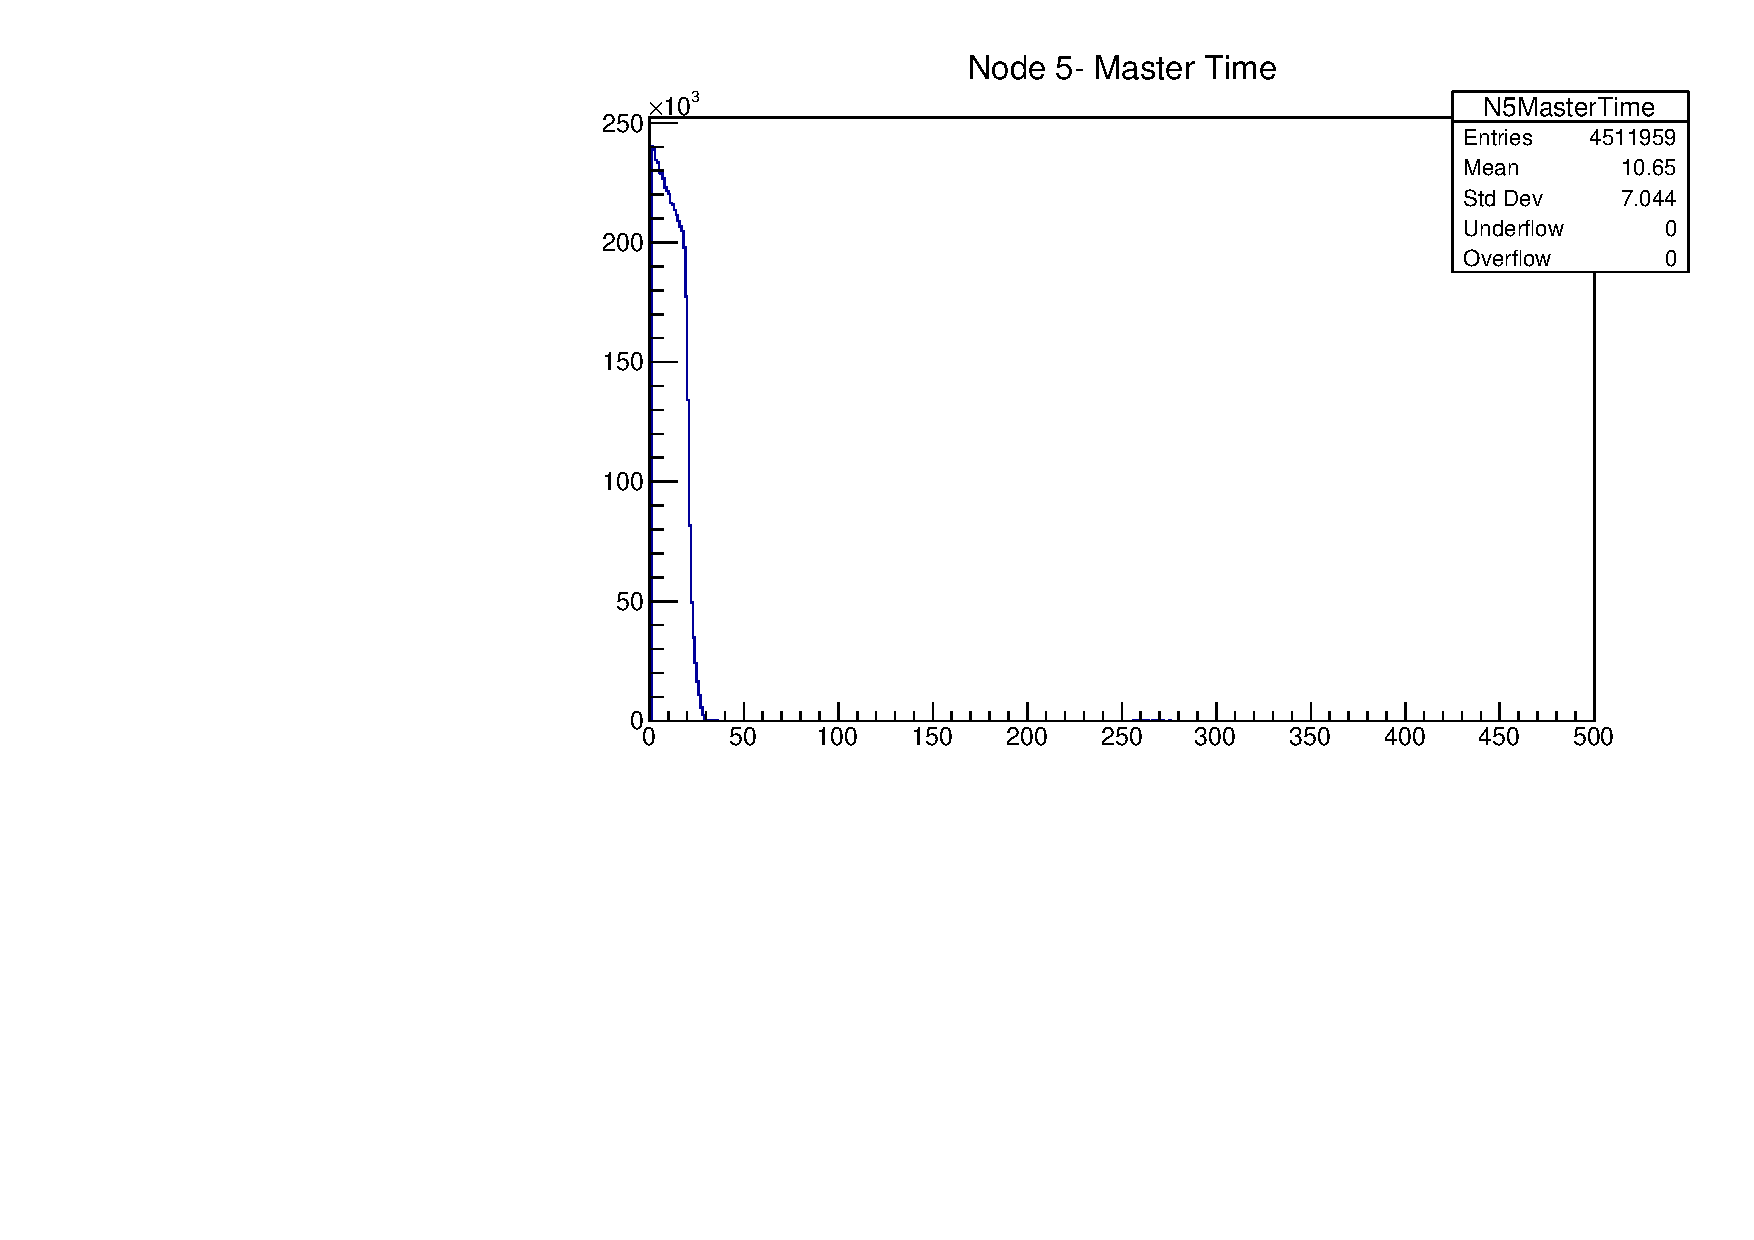
\includegraphics[width=0.33\textwidth,scale=0.5,trim=0 0 0 0,clip]{plotsdir/file0_test-N5MasterTime-1.pdf} 
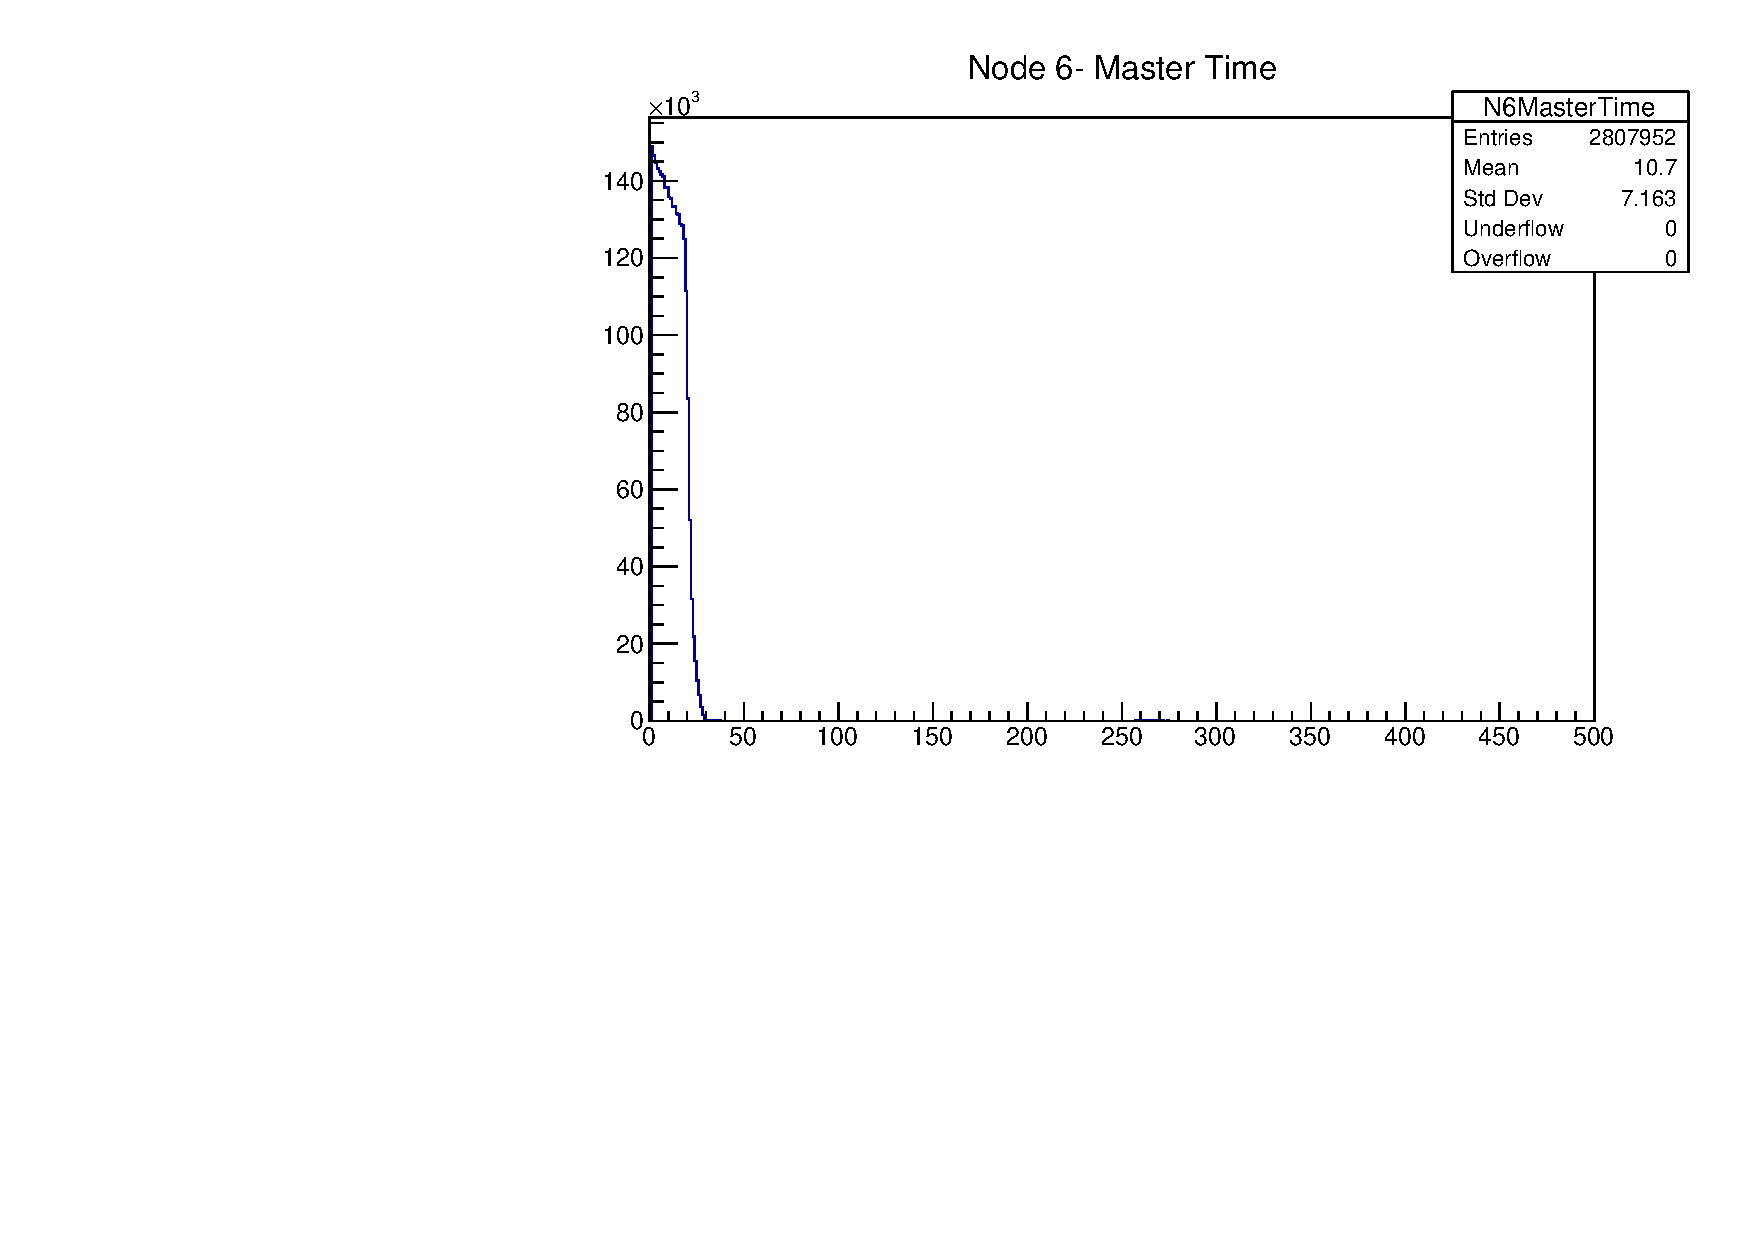
\includegraphics[width=0.33\textwidth,scale=0.5,trim=0 0 0 0,clip]{plotsdir/file0_test-N6MasterTime-1.pdf} 
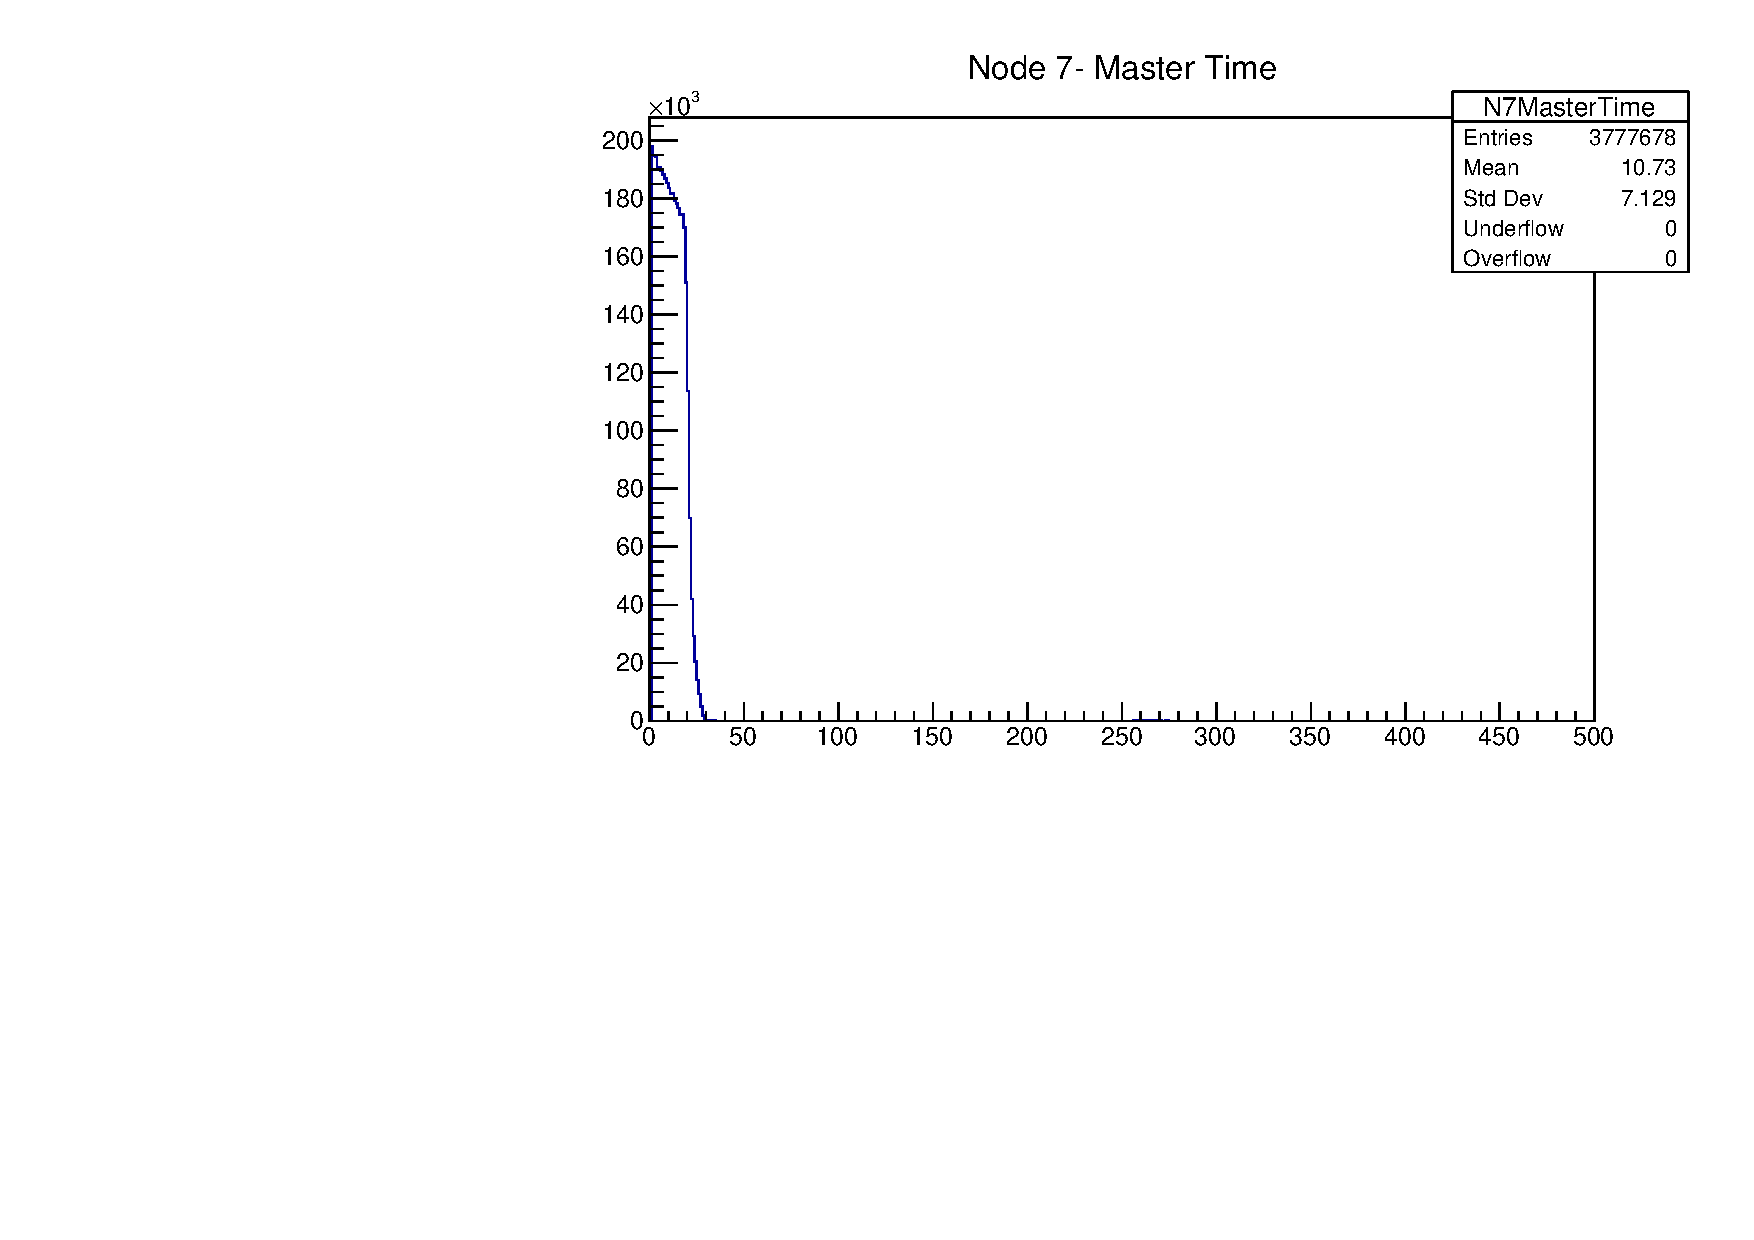
\includegraphics[width=0.33\textwidth,scale=0.5,trim=0 0 0 0,clip]{plotsdir/file0_test-N7MasterTime-1.pdf} 
\caption{(a)Node 5- Master Time ~~~(b) Node 6- Master Time ~~~(c)Node 7- Master Time } 
\end{figure} 
\begin{figure}[H] 
\vspace*{-0.3cm} 
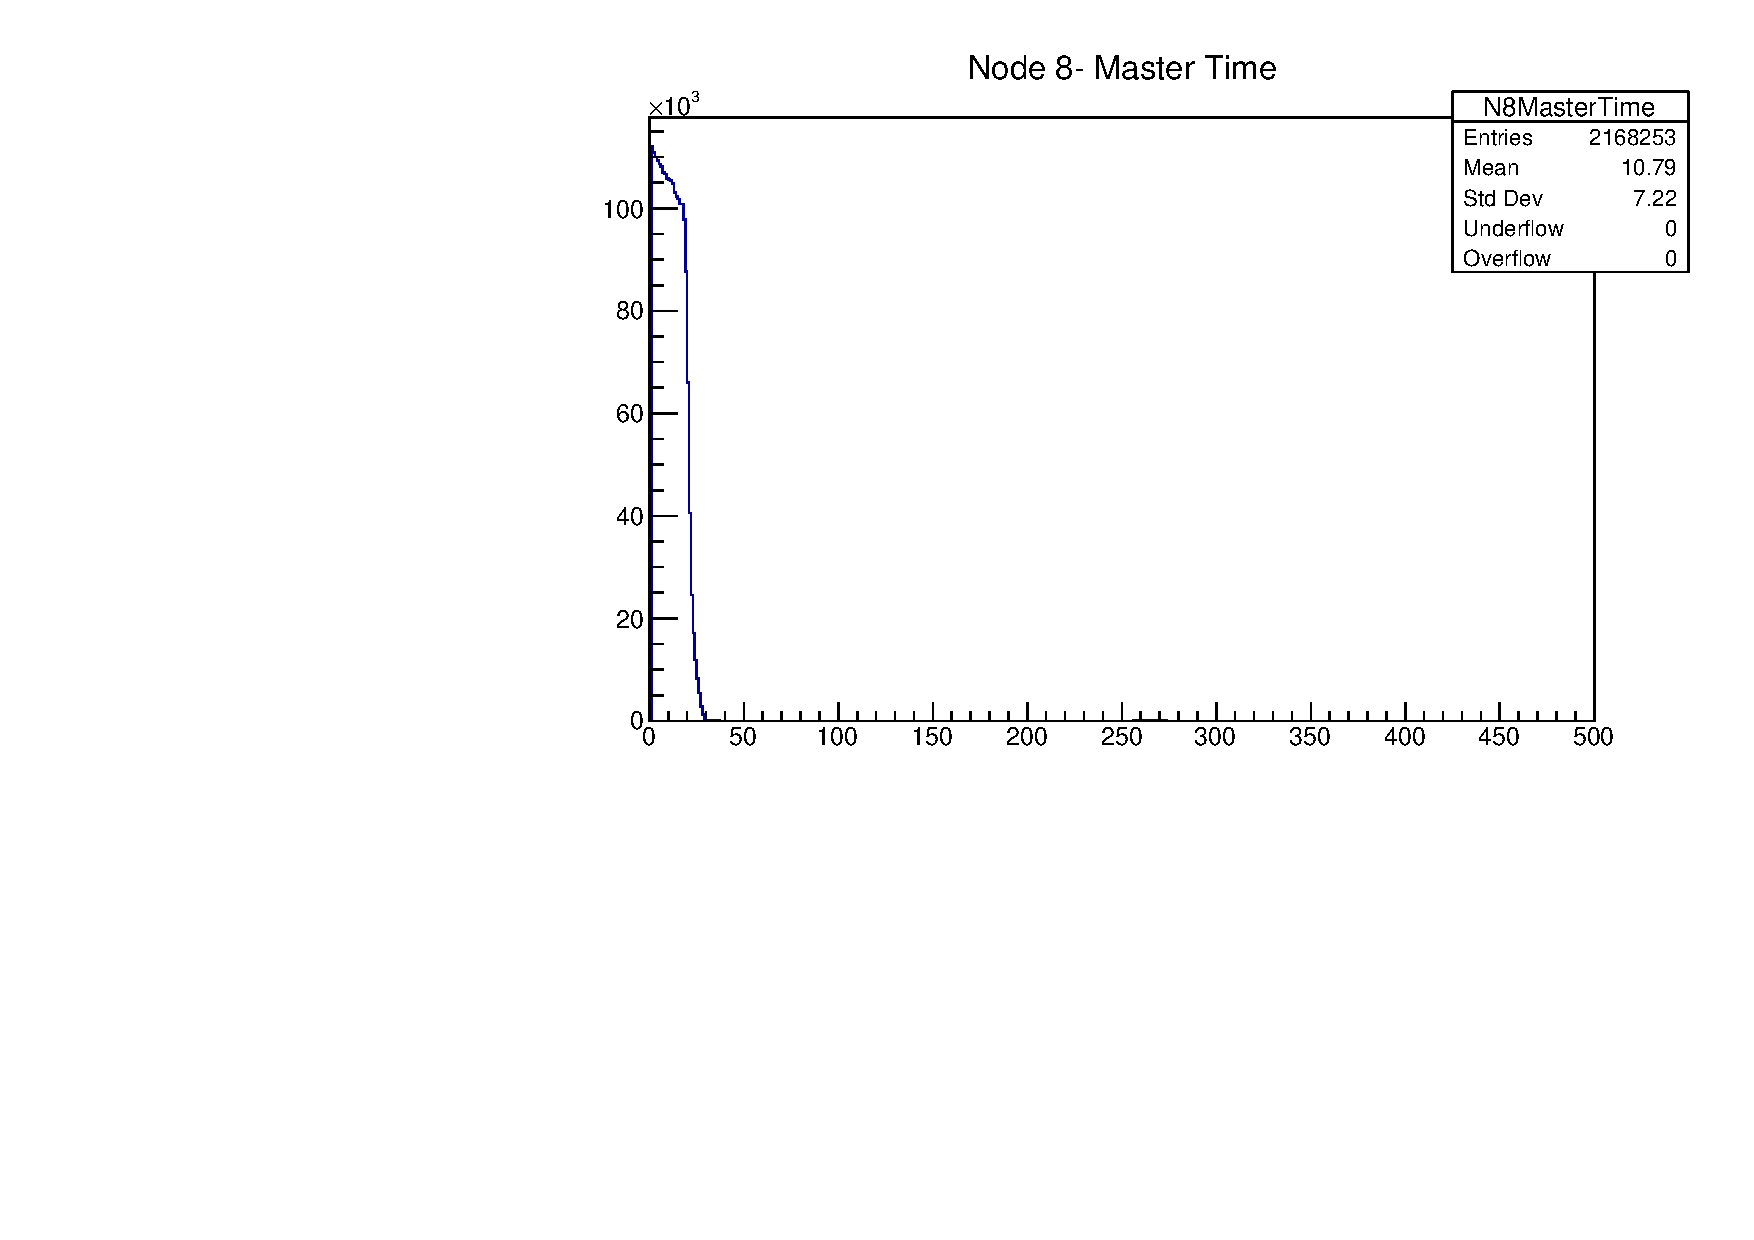
\includegraphics[width=0.33\textwidth,scale=0.5,trim=0 0 0 0,clip]{plotsdir/file0_test-N8MasterTime-1.pdf} 
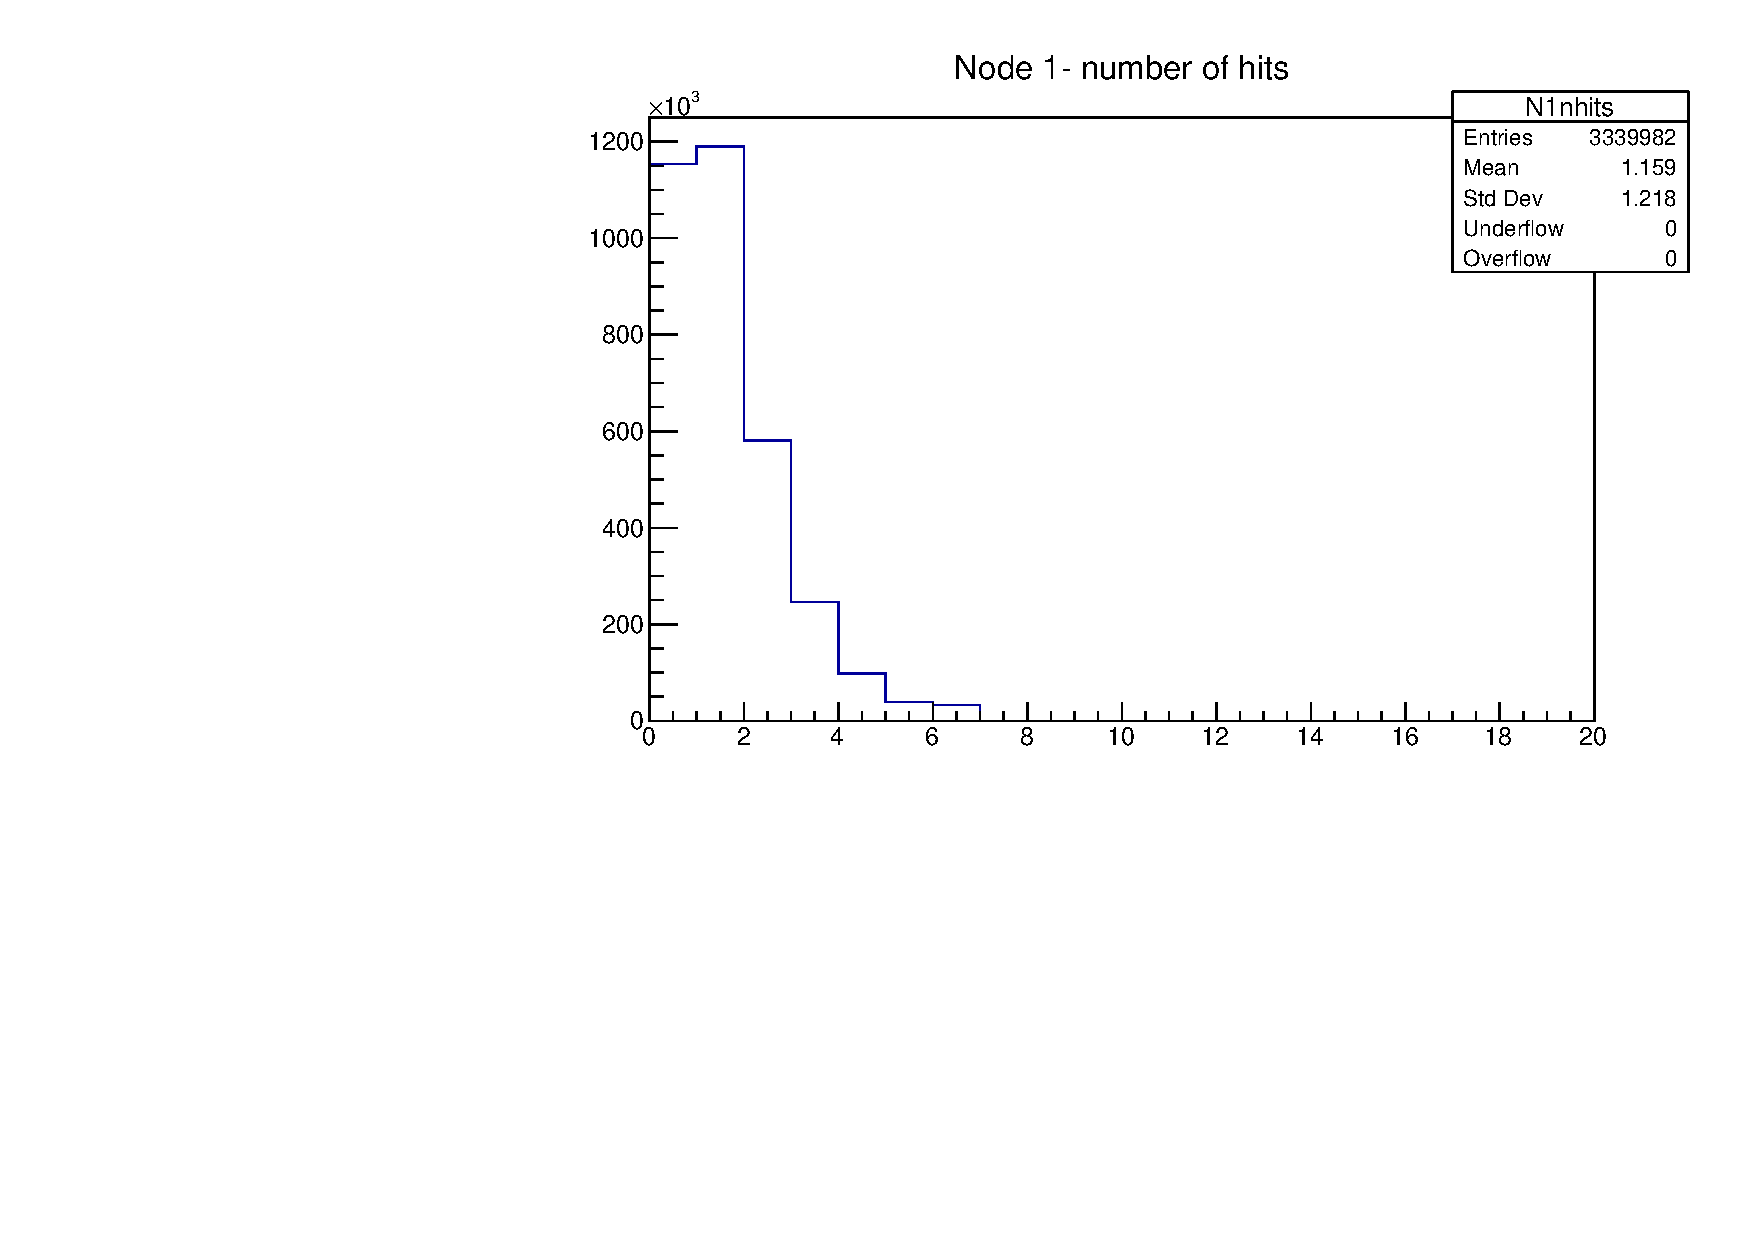
\includegraphics[width=0.33\textwidth,scale=0.5,trim=0 0 0 0,clip]{plotsdir/file0_test-N1nhits-1.pdf} 
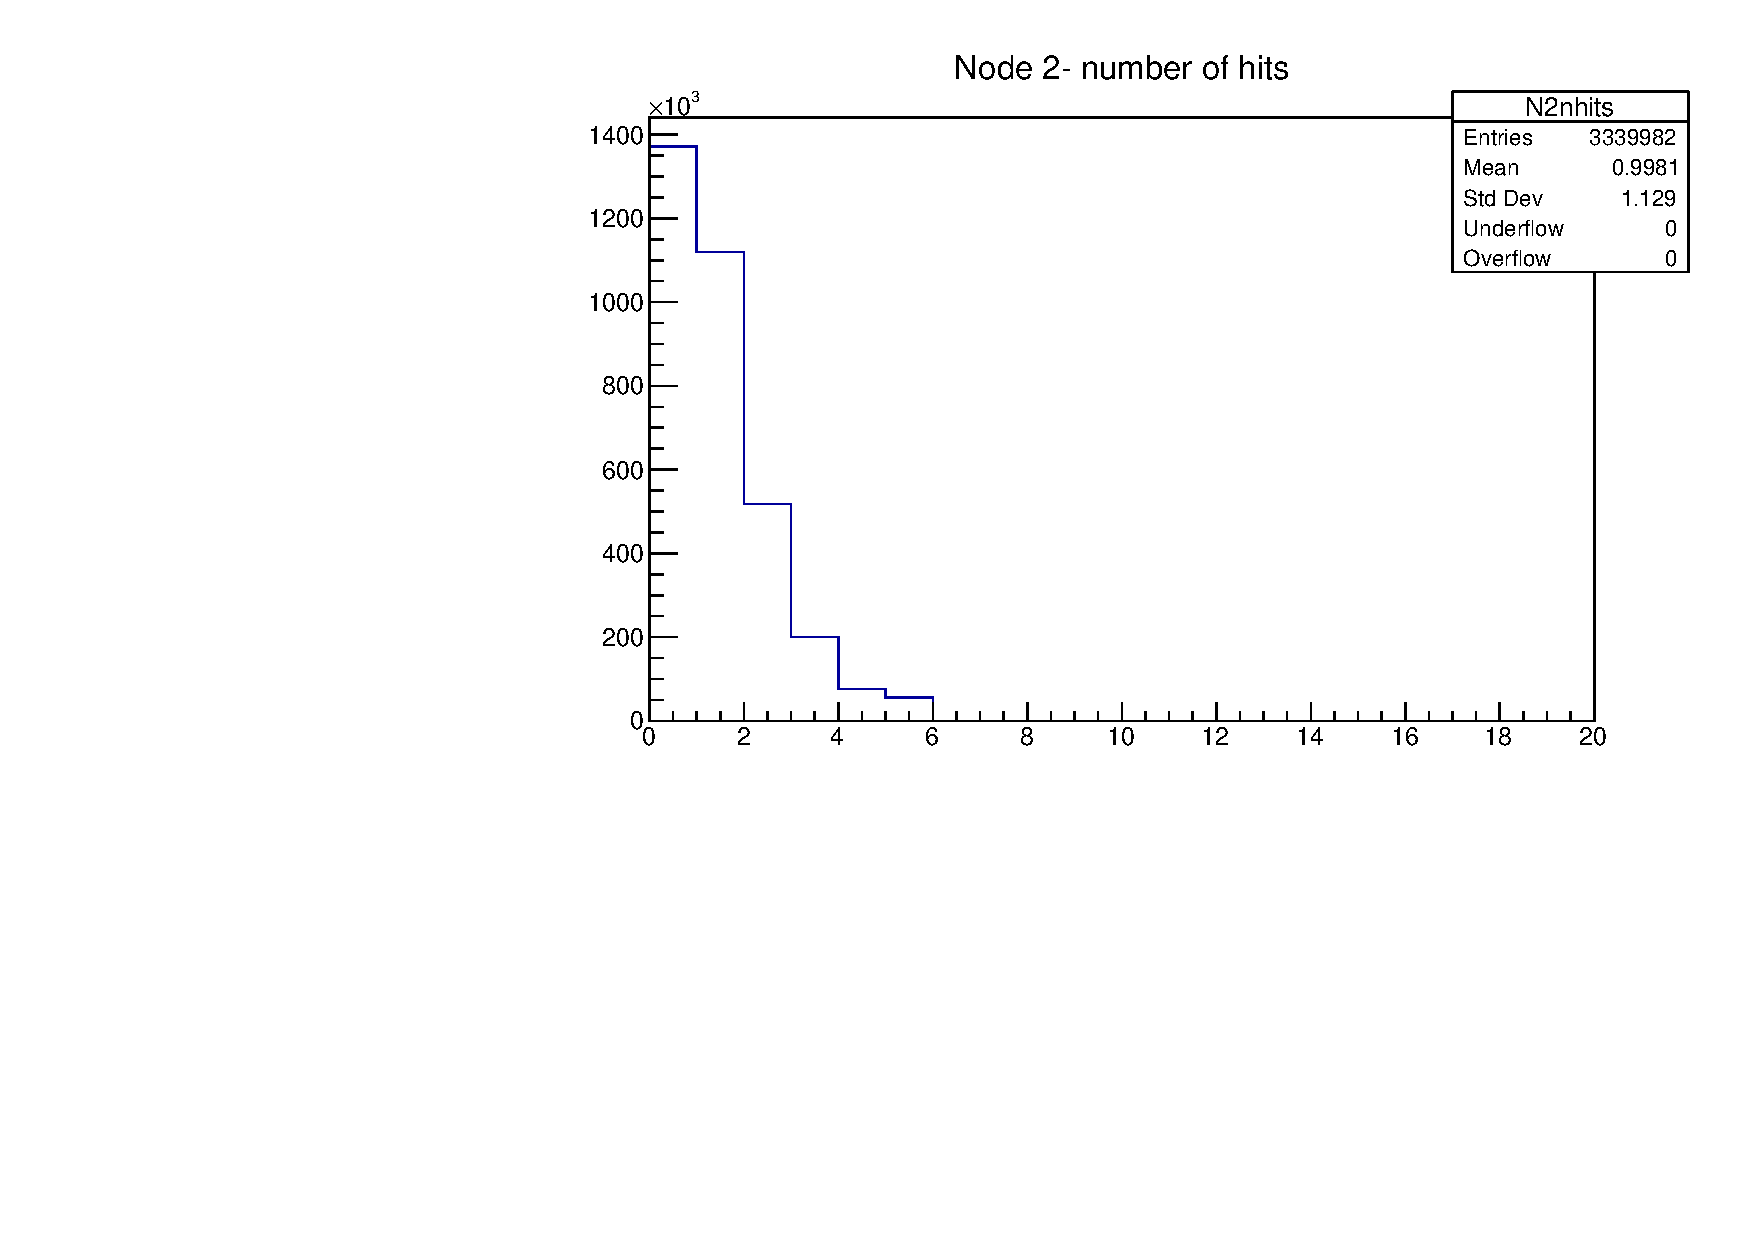
\includegraphics[width=0.33\textwidth,scale=0.5,trim=0 0 0 0,clip]{plotsdir/file0_test-N2nhits-1.pdf} 
\caption{(a)Node 8- Master Time ~~~(b) Node 1- number of hits ~~~(c)Node 2- number of hits } 
\end{figure} 
\begin{figure}[H] 
\vspace*{-0.3cm} 
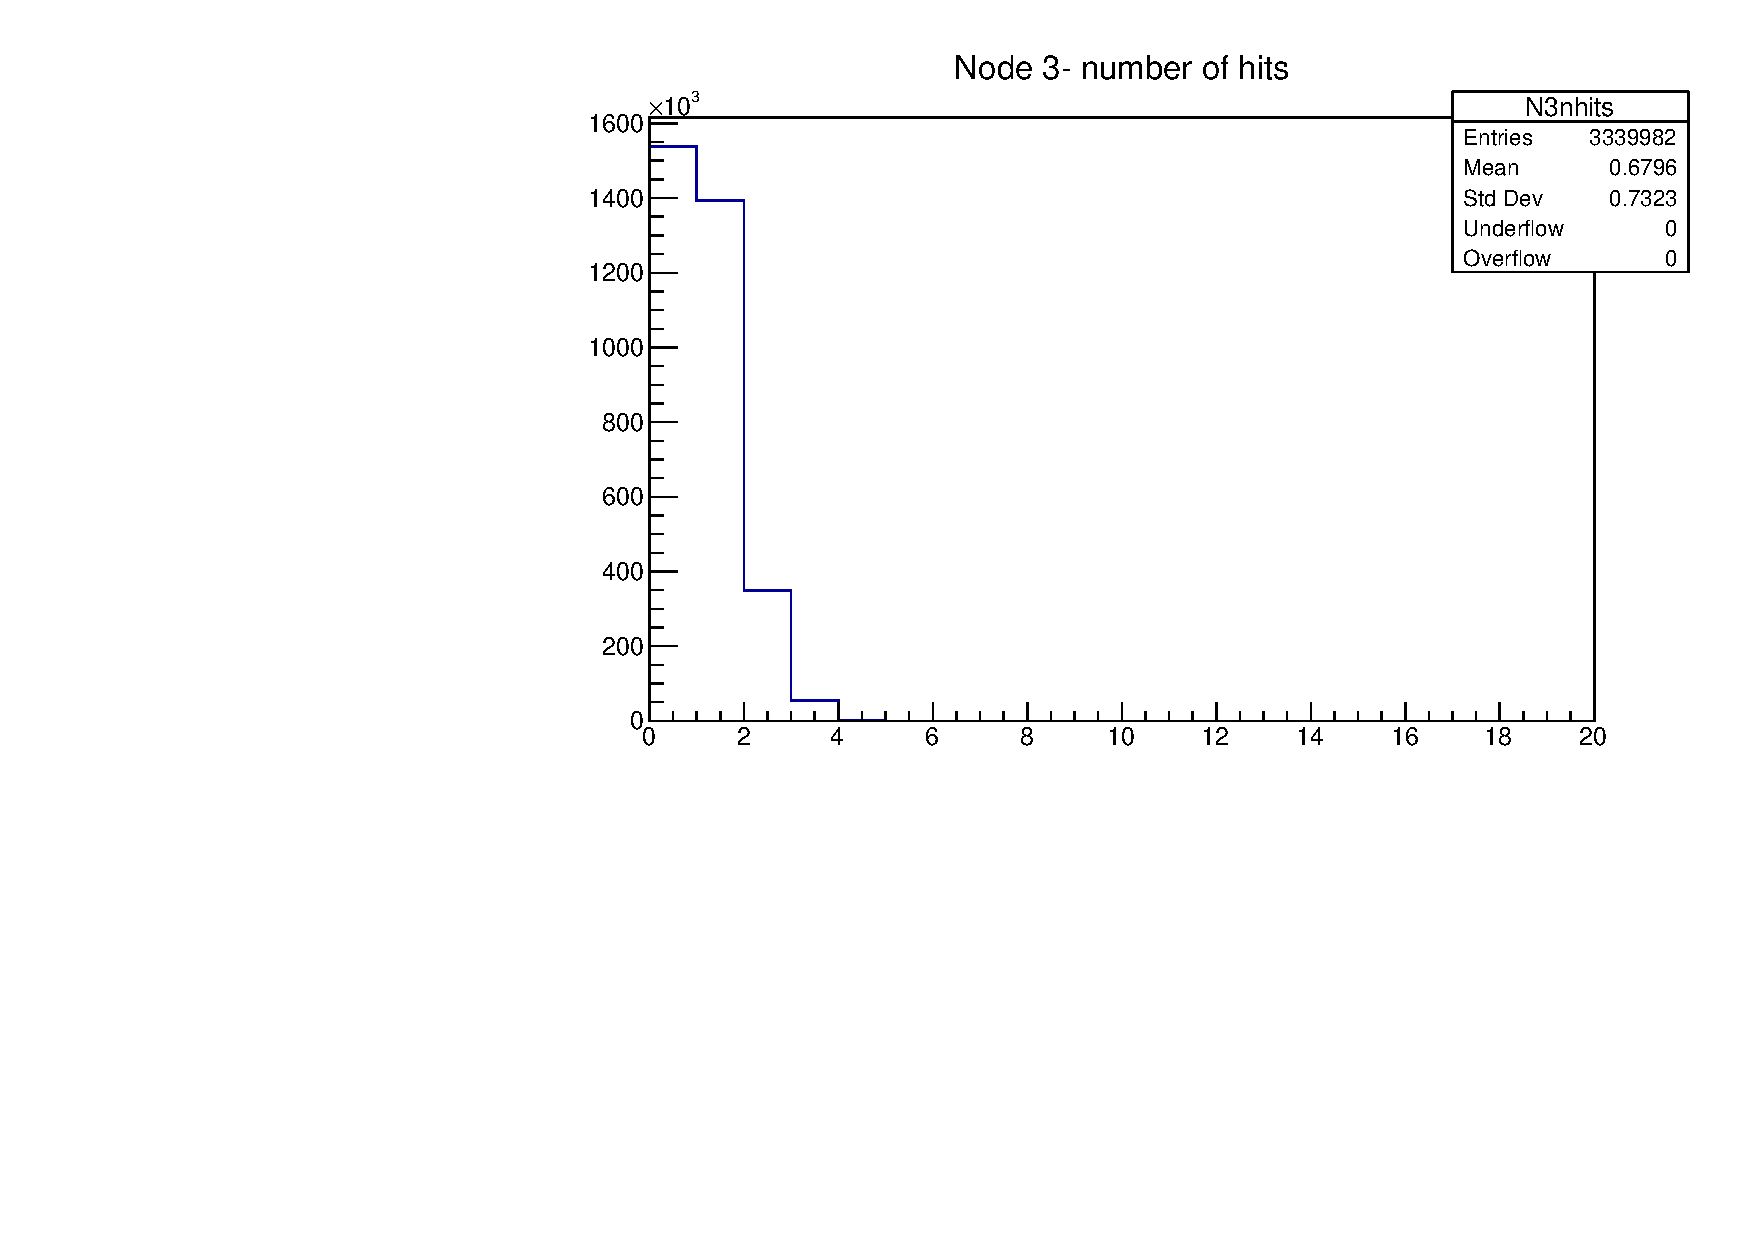
\includegraphics[width=0.33\textwidth,scale=0.5,trim=0 0 0 0,clip]{plotsdir/file0_test-N3nhits-1.pdf} 
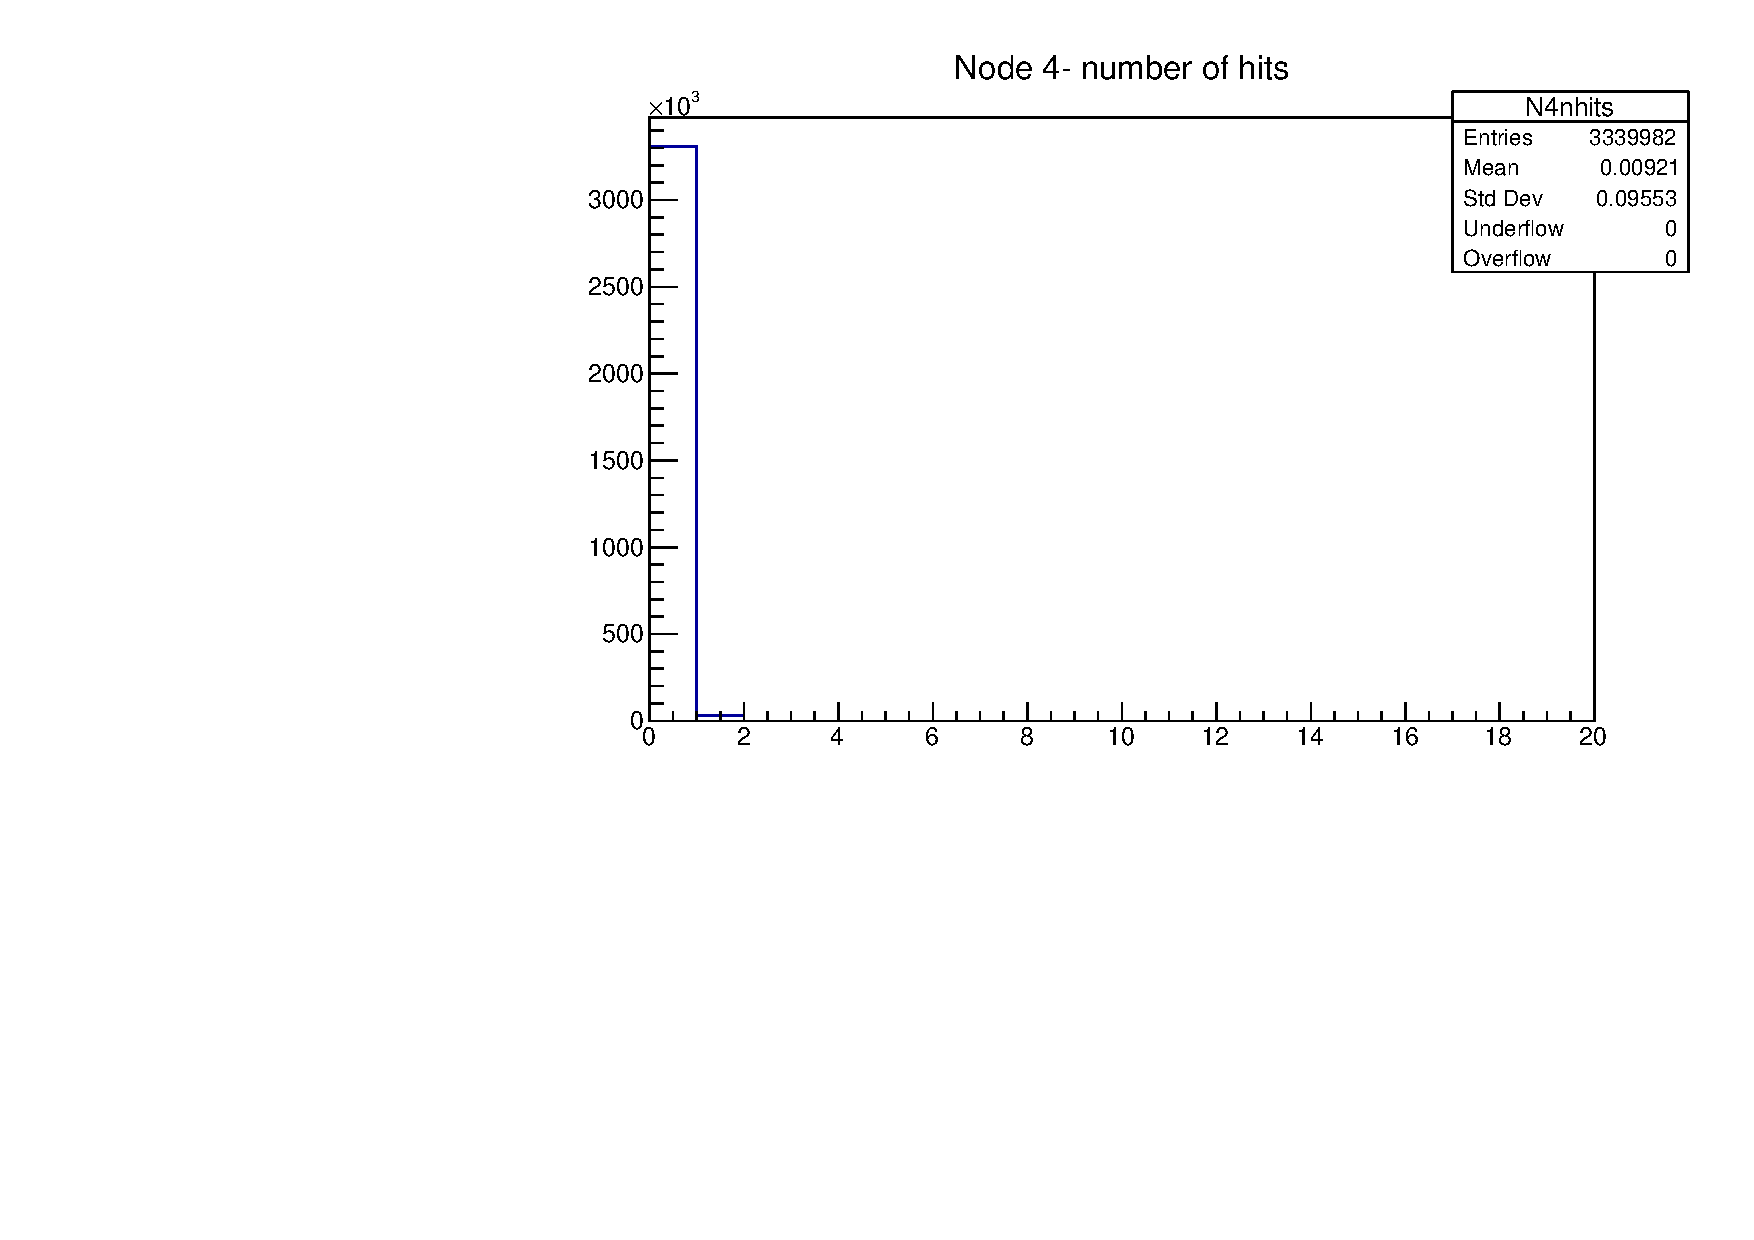
\includegraphics[width=0.33\textwidth,scale=0.5,trim=0 0 0 0,clip]{plotsdir/file0_test-N4nhits-1.pdf} 
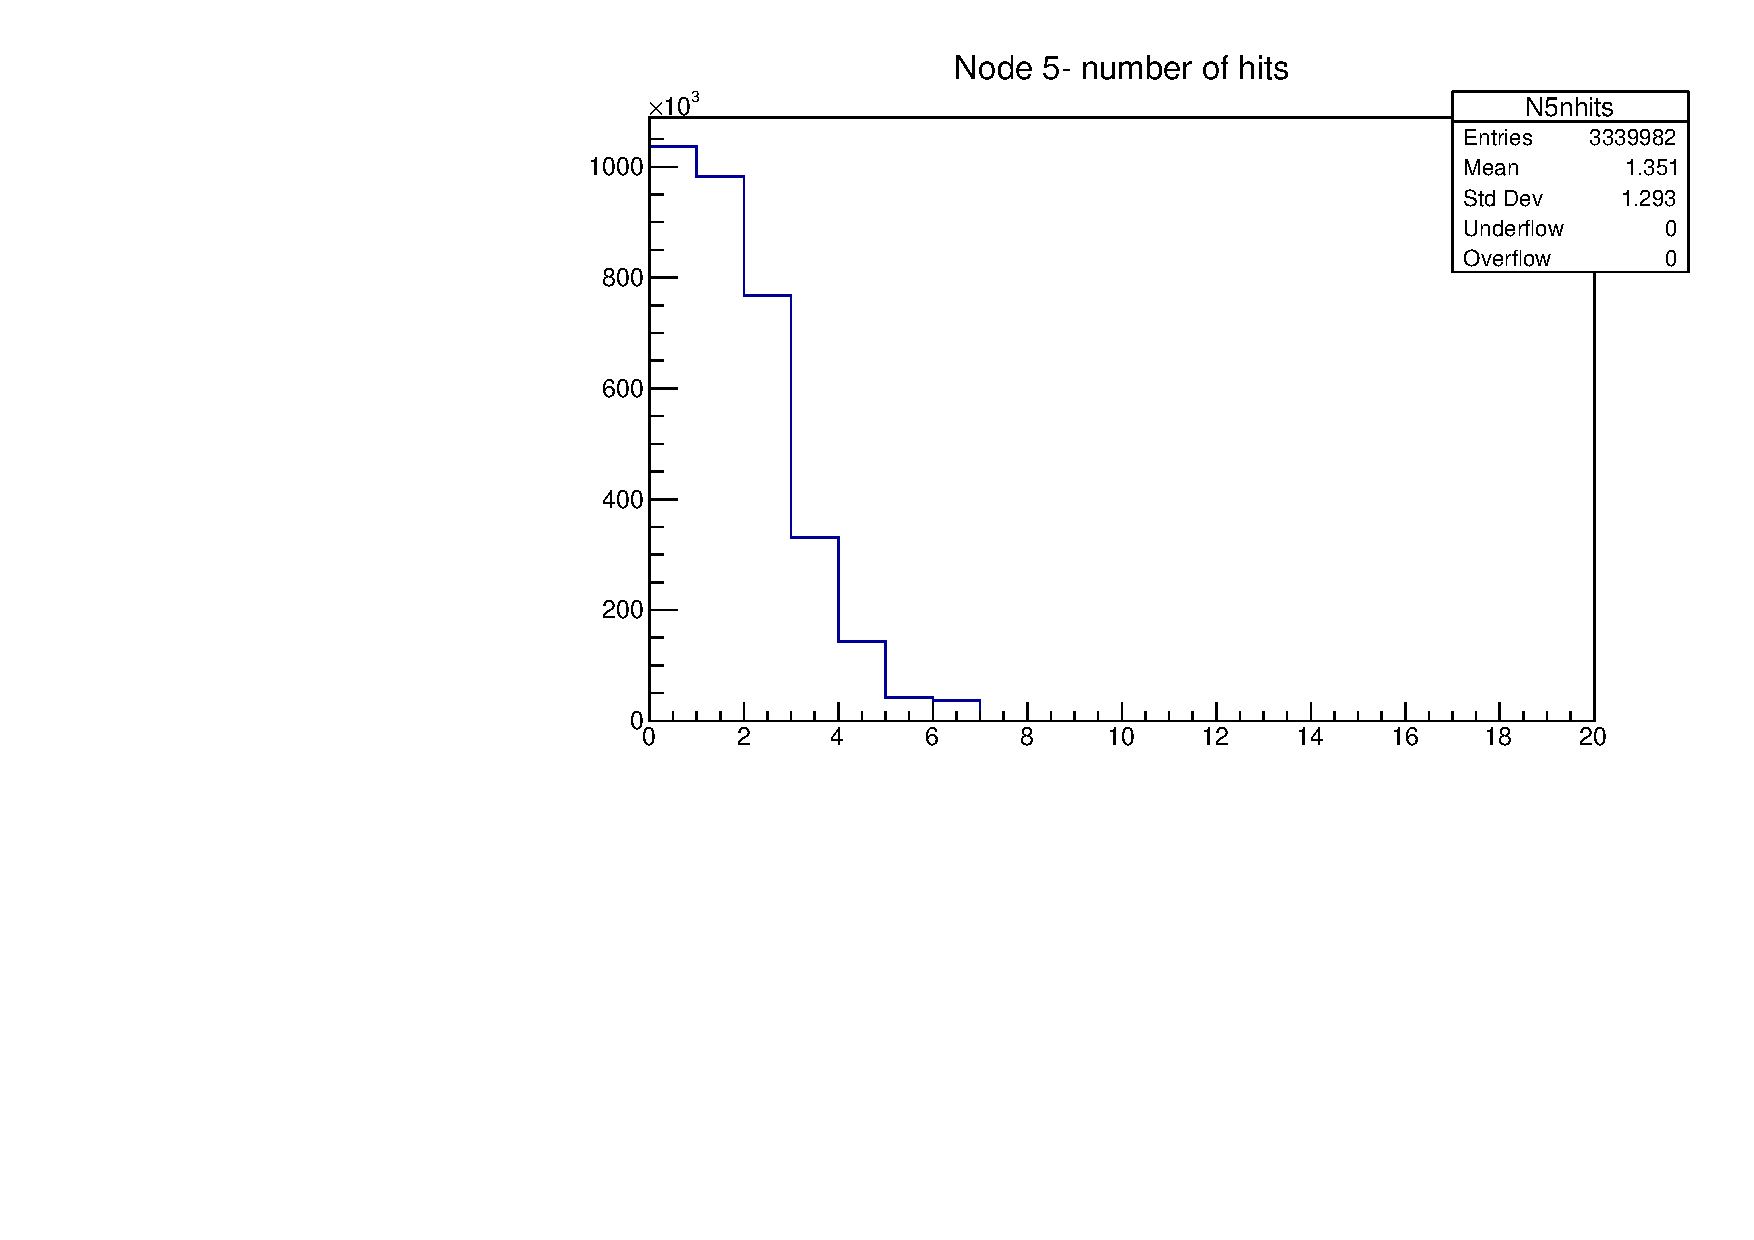
\includegraphics[width=0.33\textwidth,scale=0.5,trim=0 0 0 0,clip]{plotsdir/file0_test-N5nhits-1.pdf} 
\caption{(a)Node 3- number of hits ~~~(b) Node 4- number of hits ~~~(c)Node 5- number of hits } 
\end{figure} 
\begin{figure}[H] 
\vspace*{-0.3cm} 
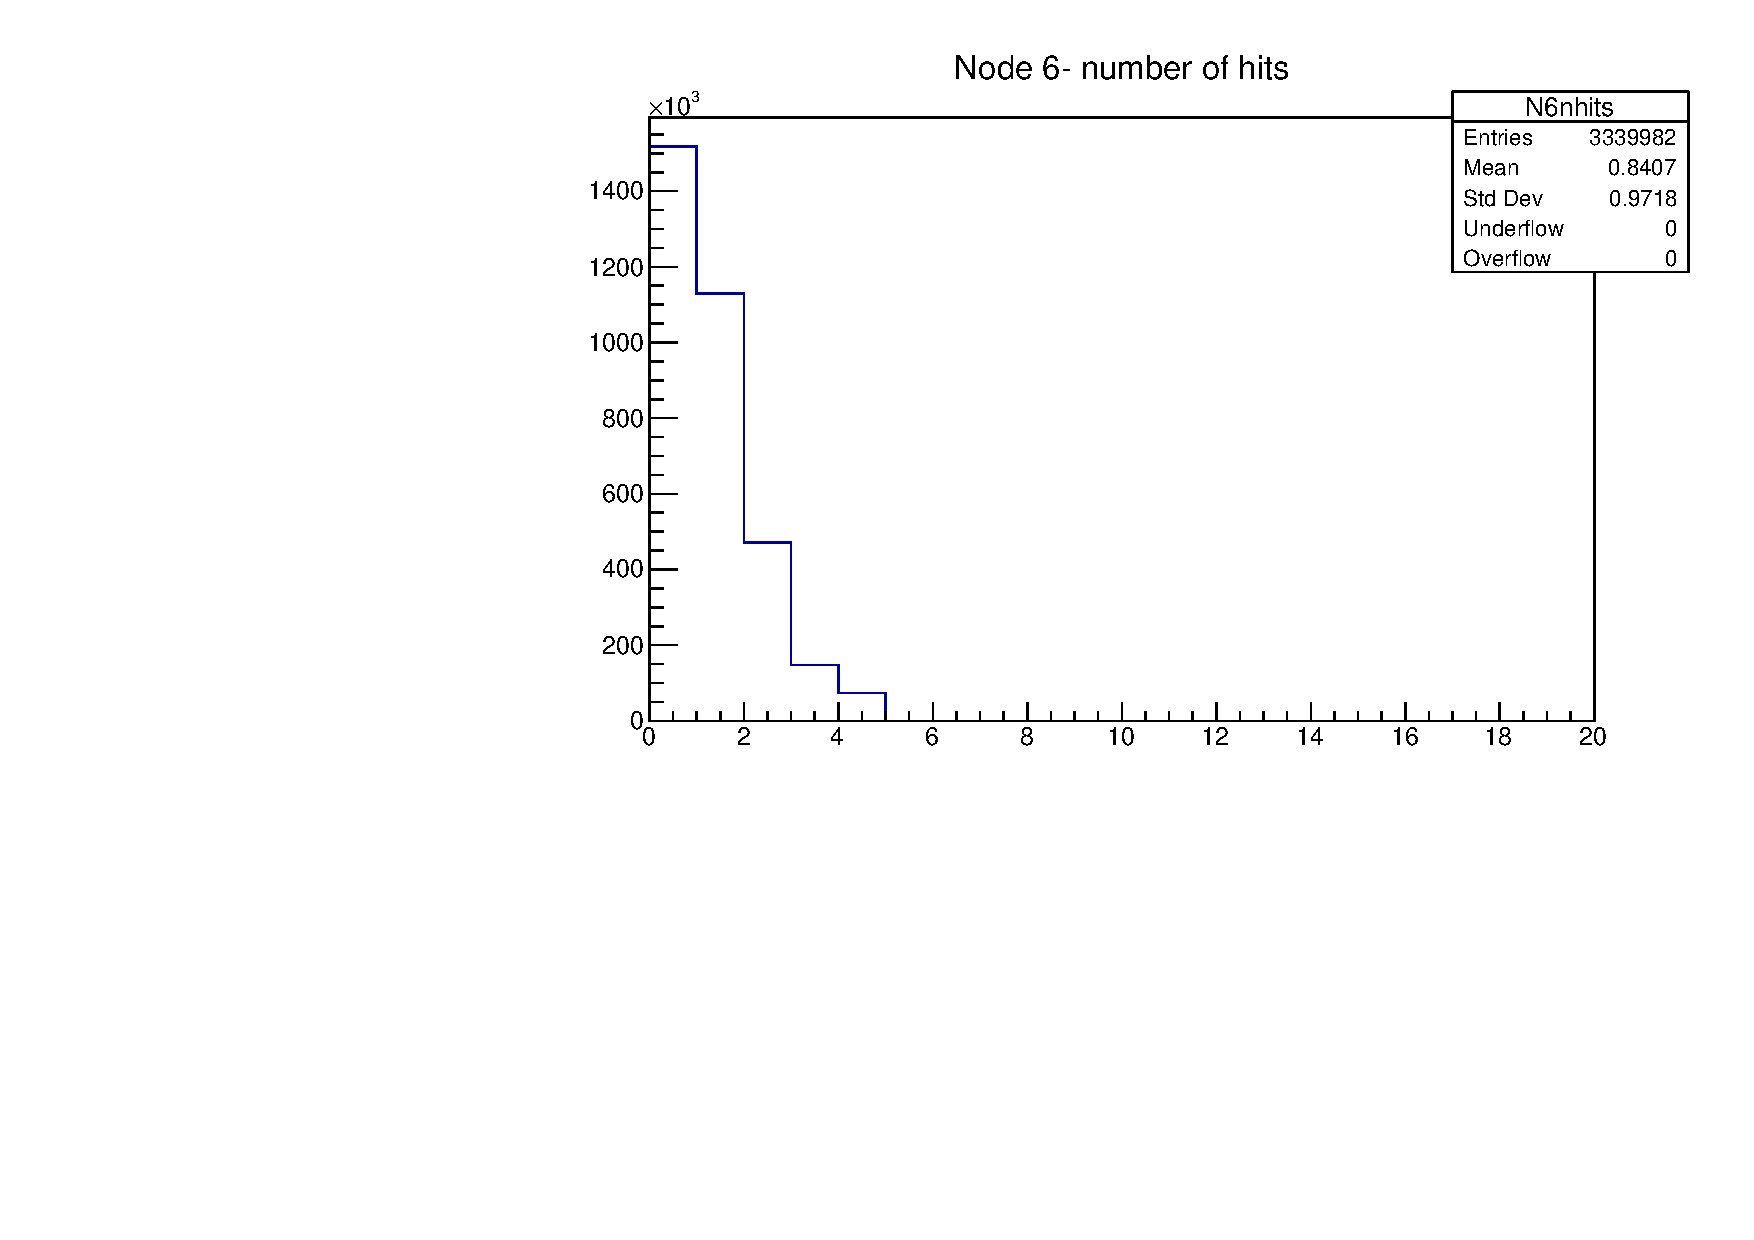
\includegraphics[width=0.33\textwidth,scale=0.5,trim=0 0 0 0,clip]{plotsdir/file0_test-N6nhits-1.pdf} 
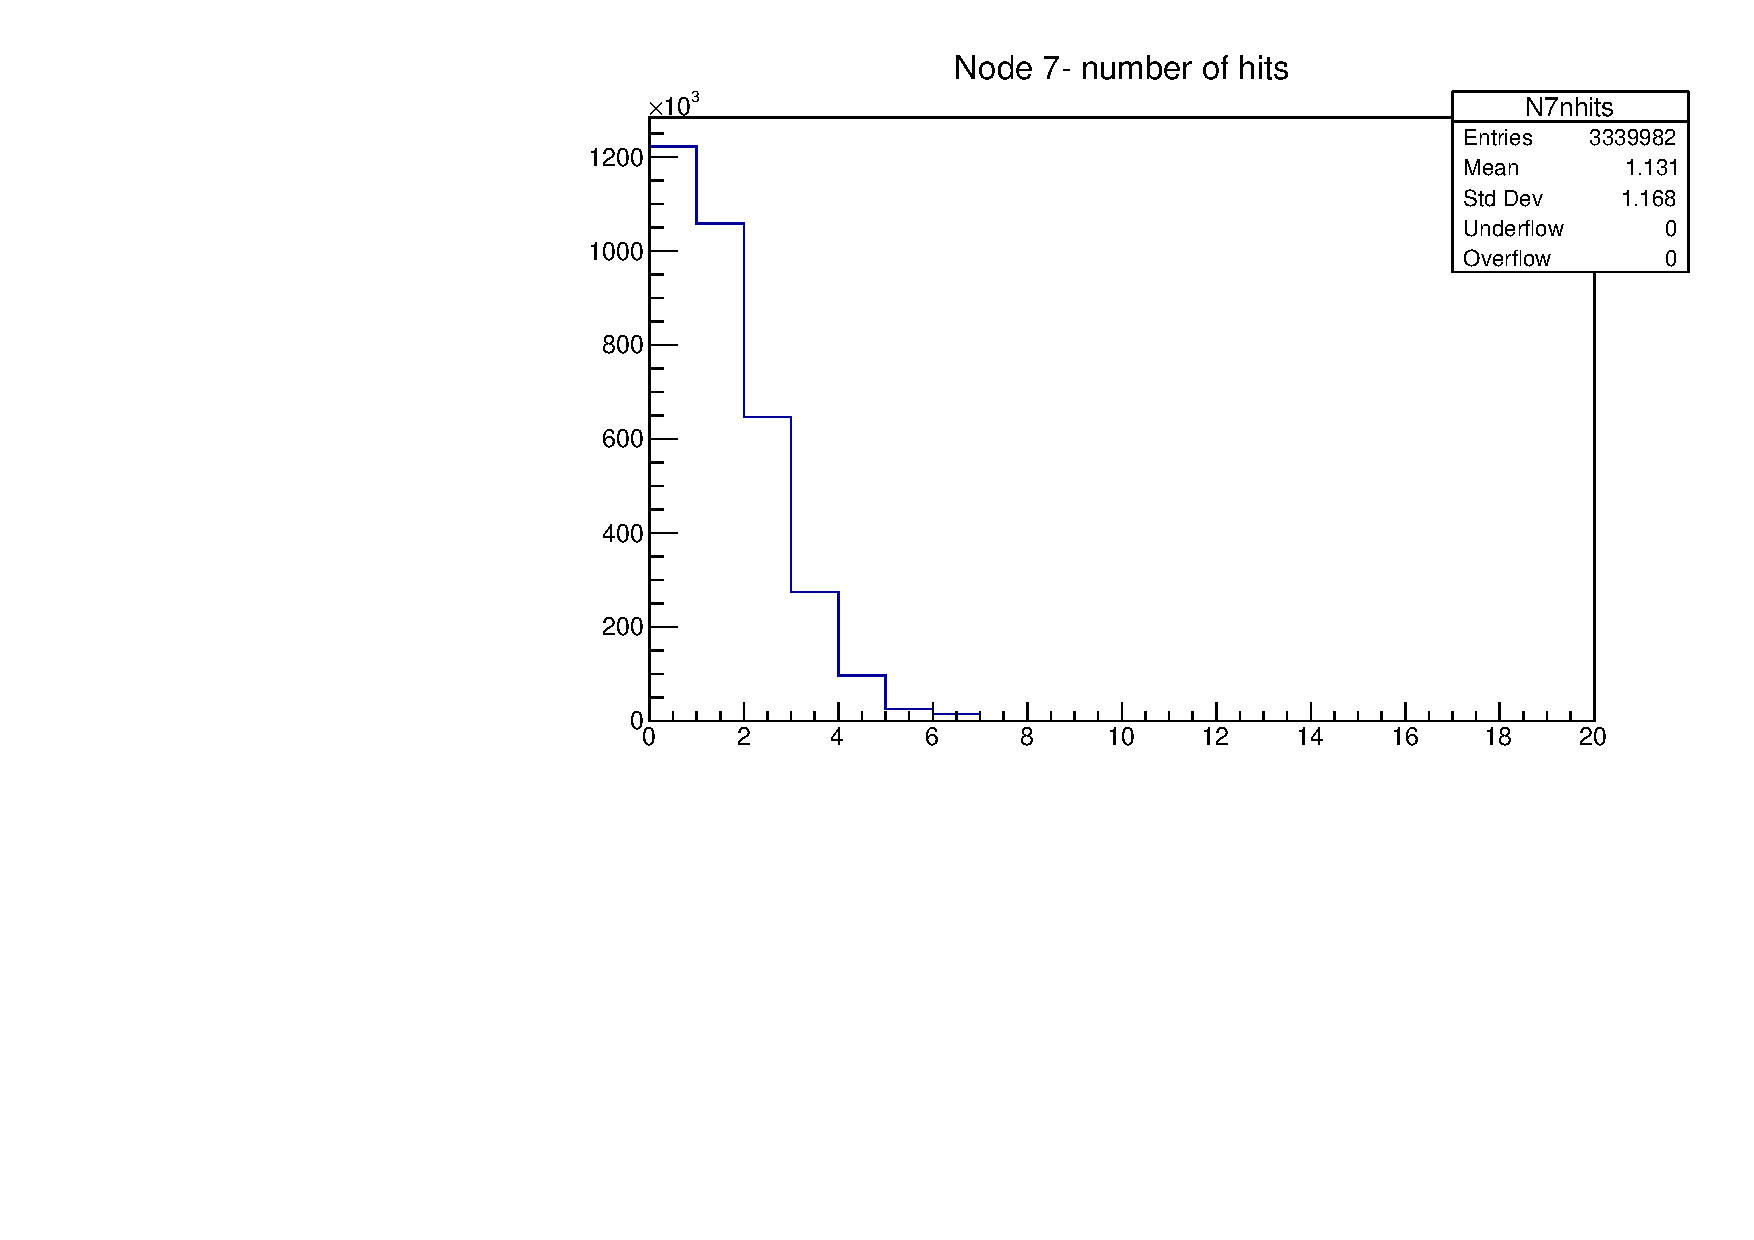
\includegraphics[width=0.33\textwidth,scale=0.5,trim=0 0 0 0,clip]{plotsdir/file0_test-N7nhits-1.pdf} 
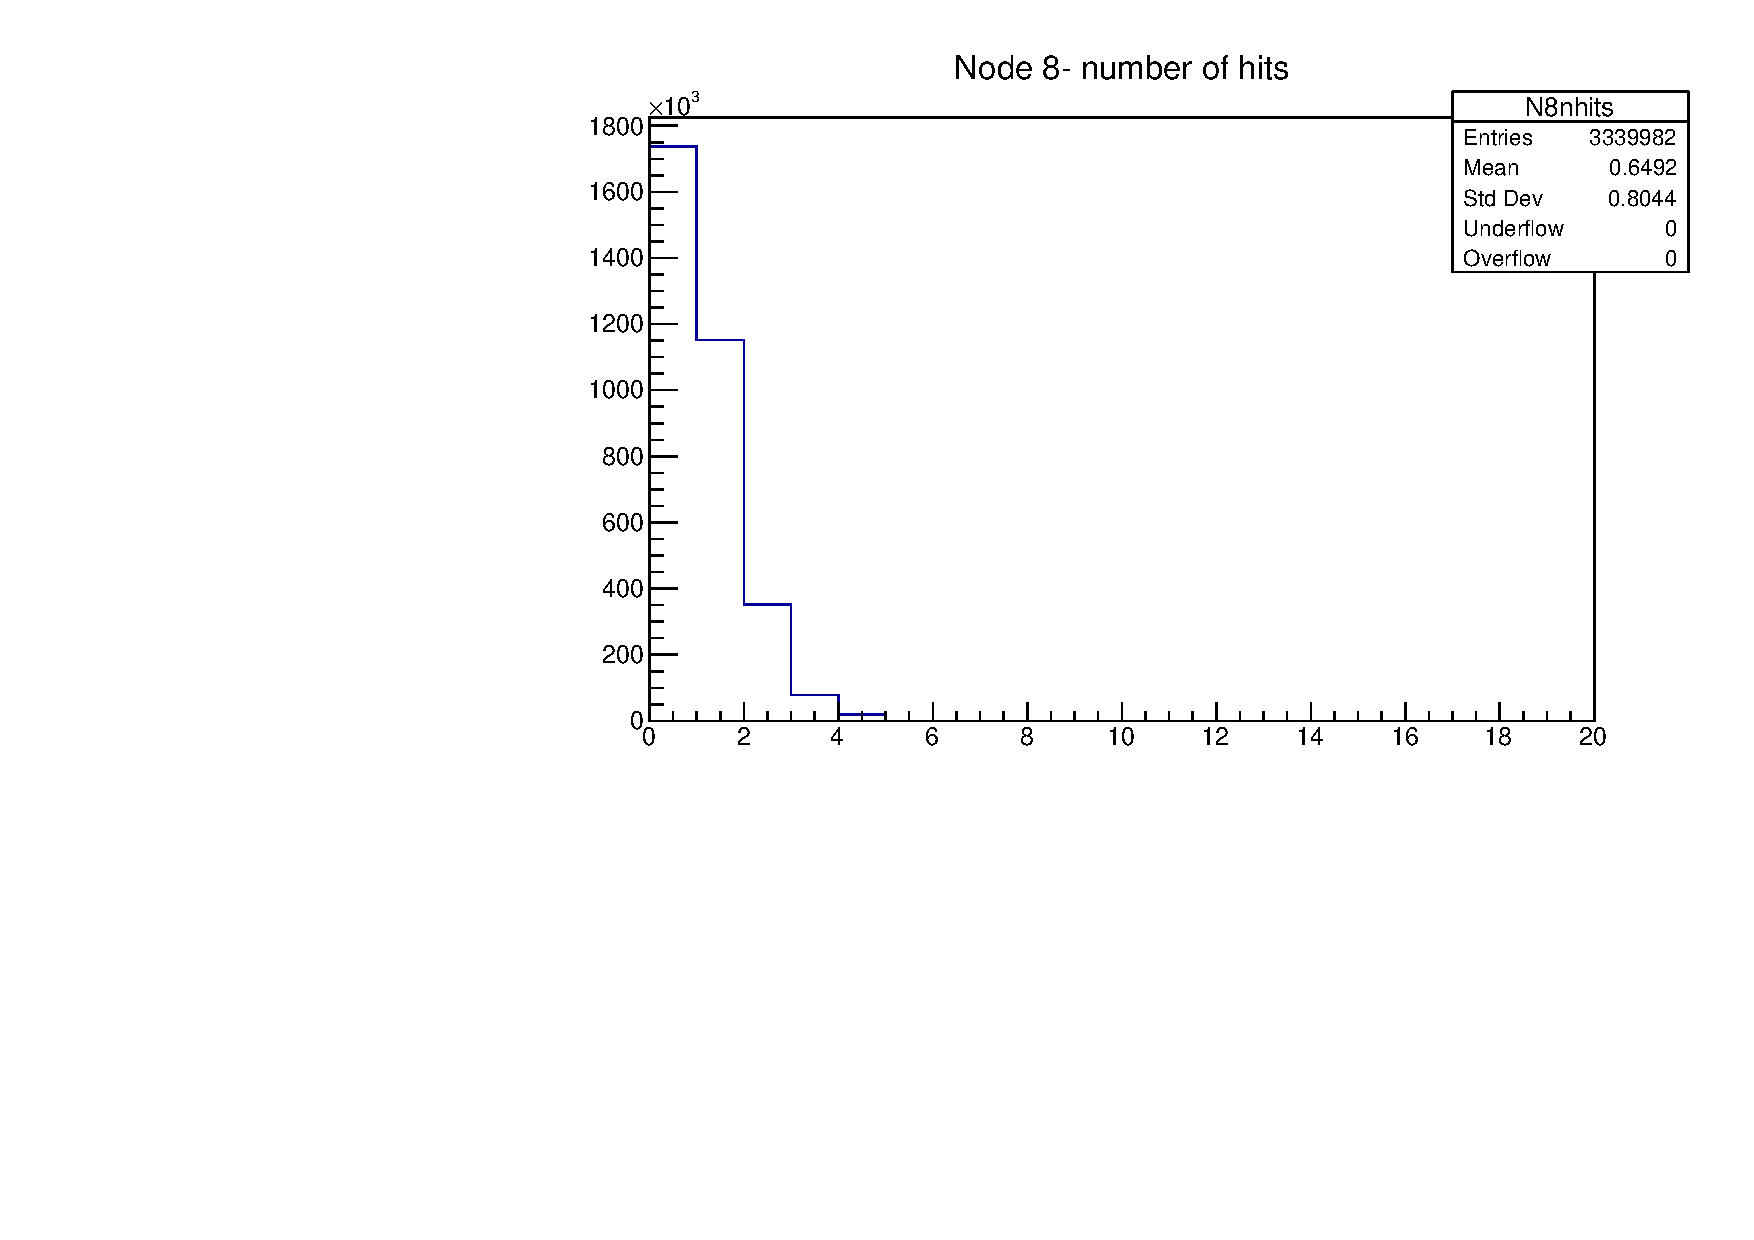
\includegraphics[width=0.33\textwidth,scale=0.5,trim=0 0 0 0,clip]{plotsdir/file0_test-N8nhits-1.pdf} 
\caption{(a)Node 6- number of hits ~~~(b) Node 7- number of hits ~~~(c)Node 8- number of hits } 
\end{figure} 
\begin{figure}[H] 
\vspace*{-0.3cm} 
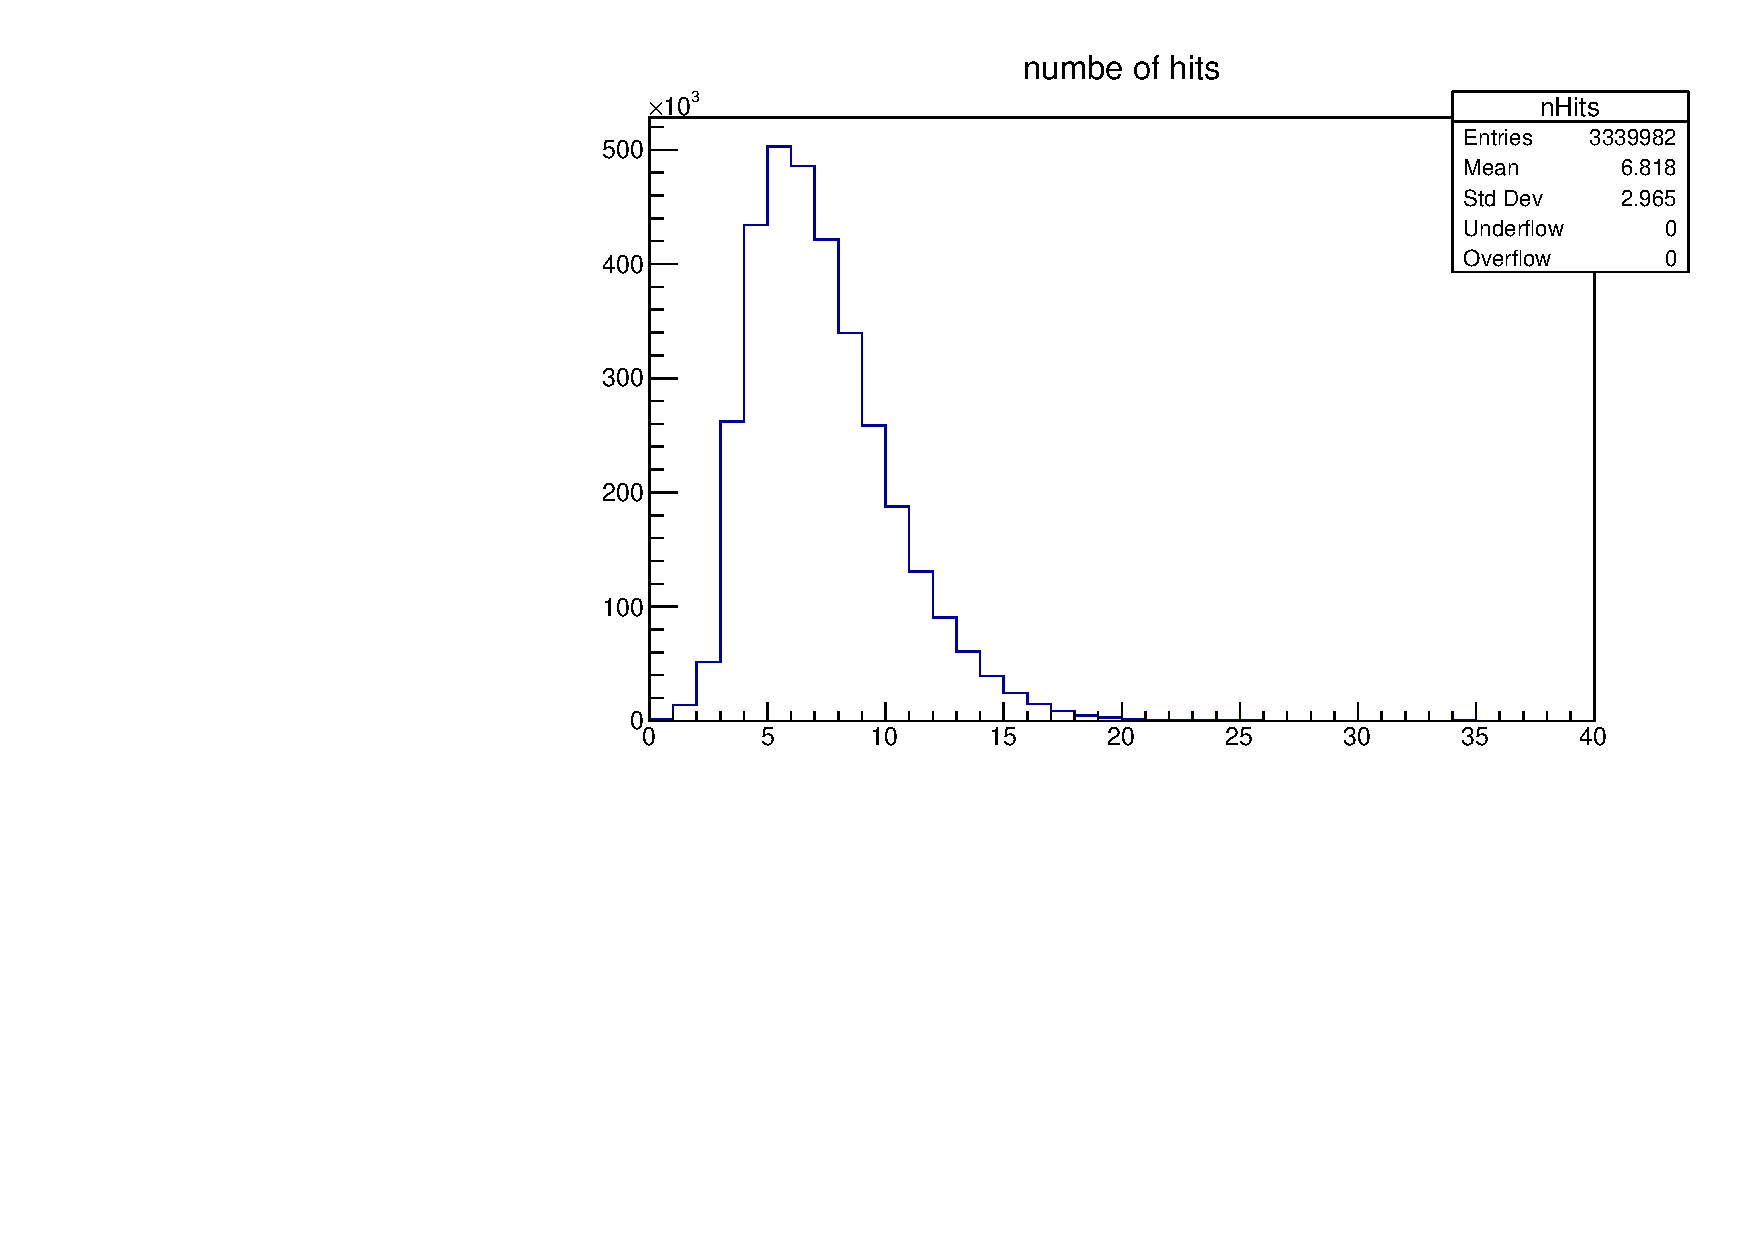
\includegraphics[width=0.33\textwidth,scale=0.5,trim=0 0 0 0,clip]{plotsdir/file0_test-nHits-1.pdf} 
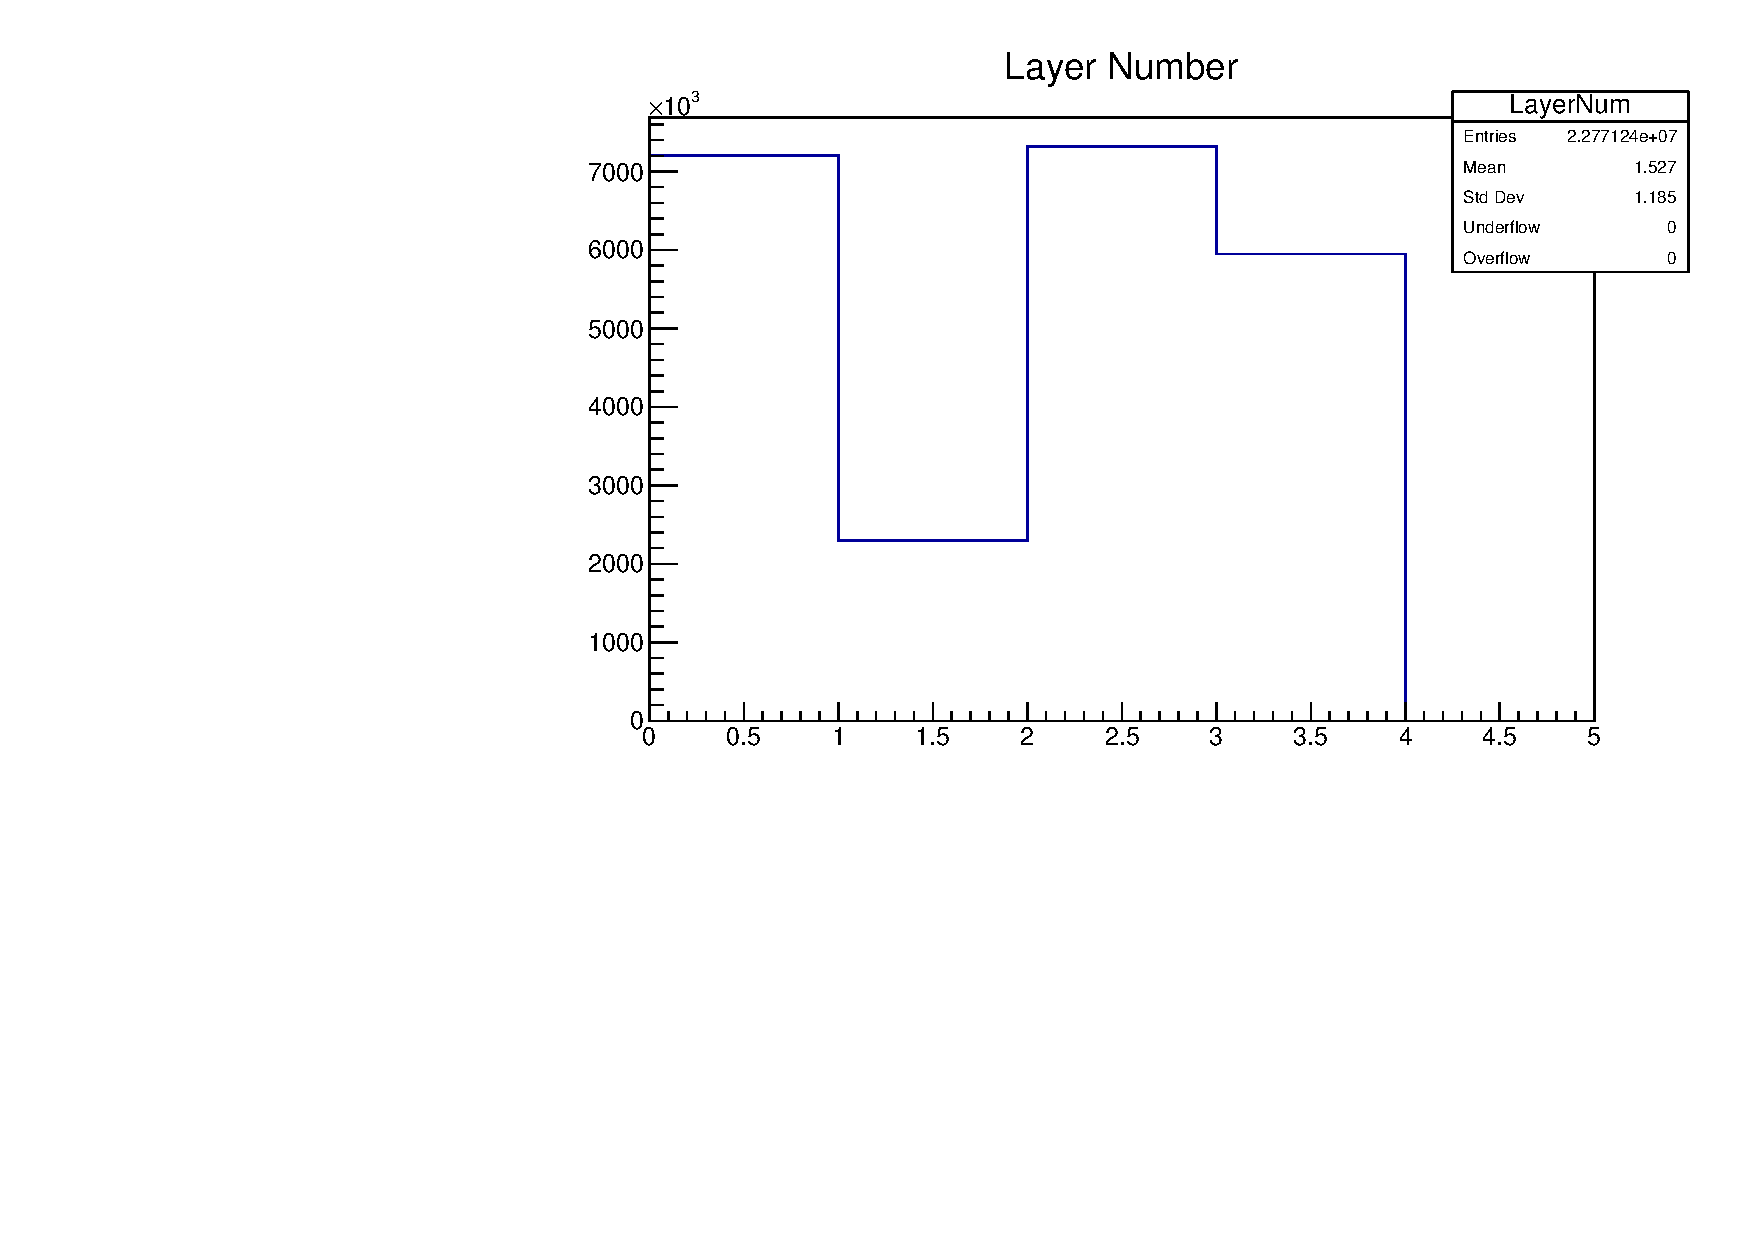
\includegraphics[width=0.33\textwidth,scale=0.5,trim=0 0 0 0,clip]{plotsdir/file0_test-LayerNum-1.pdf} 
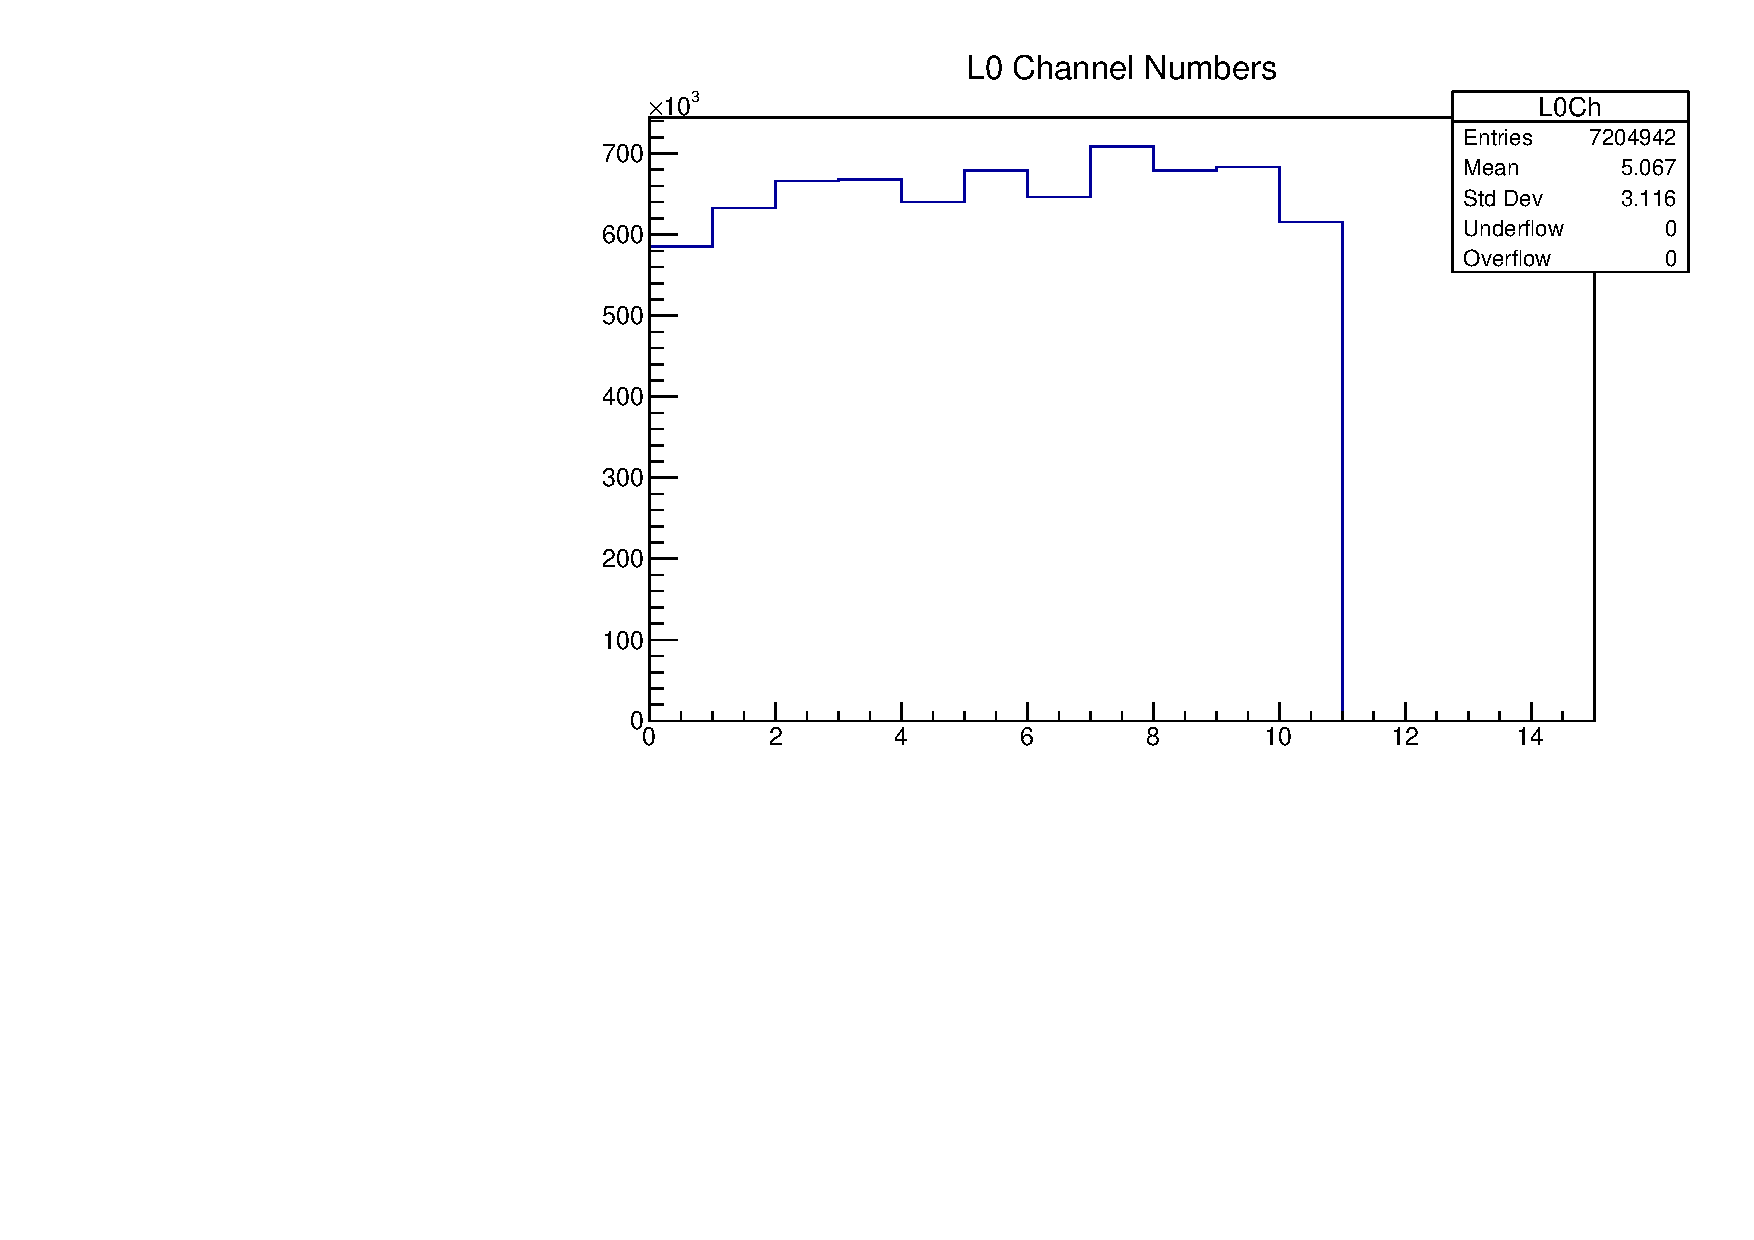
\includegraphics[width=0.33\textwidth,scale=0.5,trim=0 0 0 0,clip]{plotsdir/file0_test-L0Ch-1.pdf} 
\caption{(a)numbe of hits ~~~(b) Layer Number ~~~(c)L0 Channel Numbers } 
\end{figure} 
\begin{figure}[H] 
\vspace*{-0.3cm} 
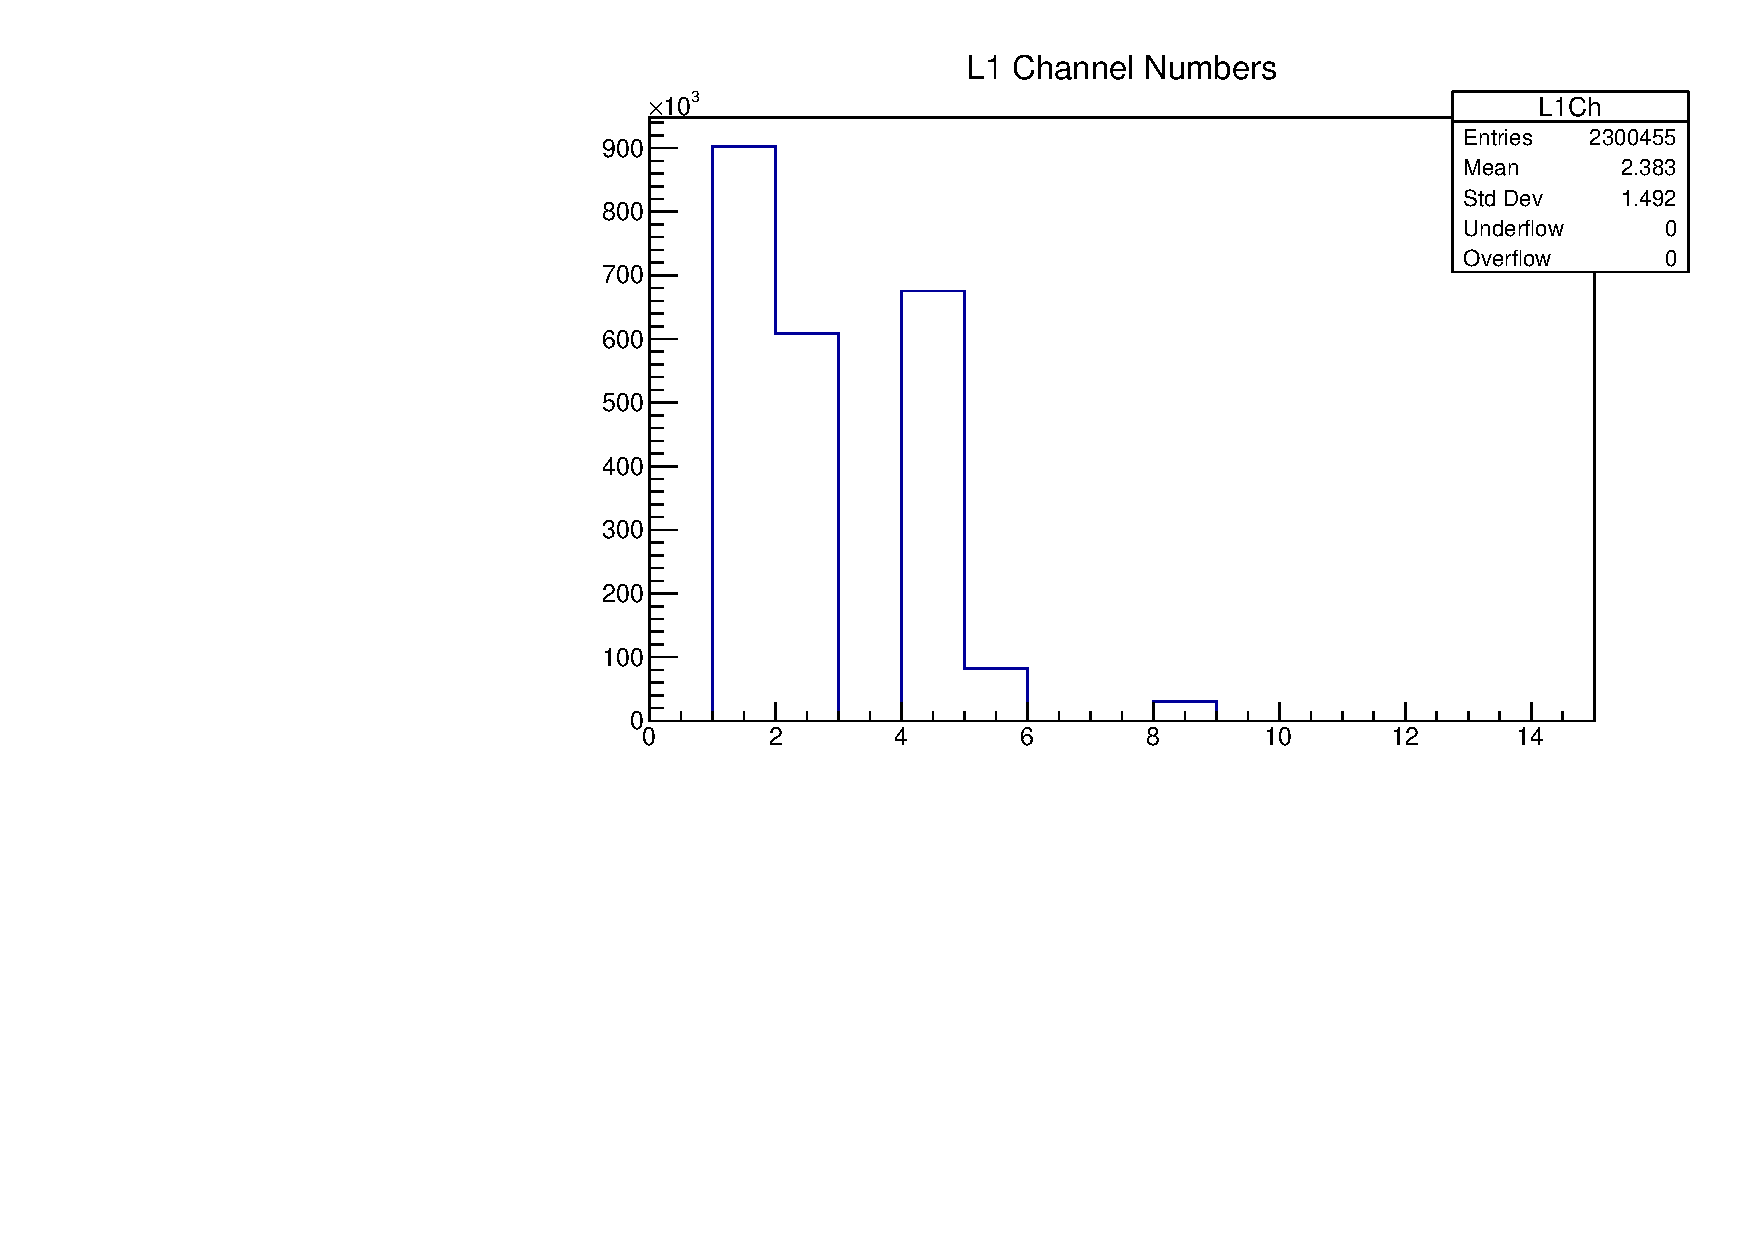
\includegraphics[width=0.33\textwidth,scale=0.5,trim=0 0 0 0,clip]{plotsdir/file0_test-L1Ch-1.pdf} 
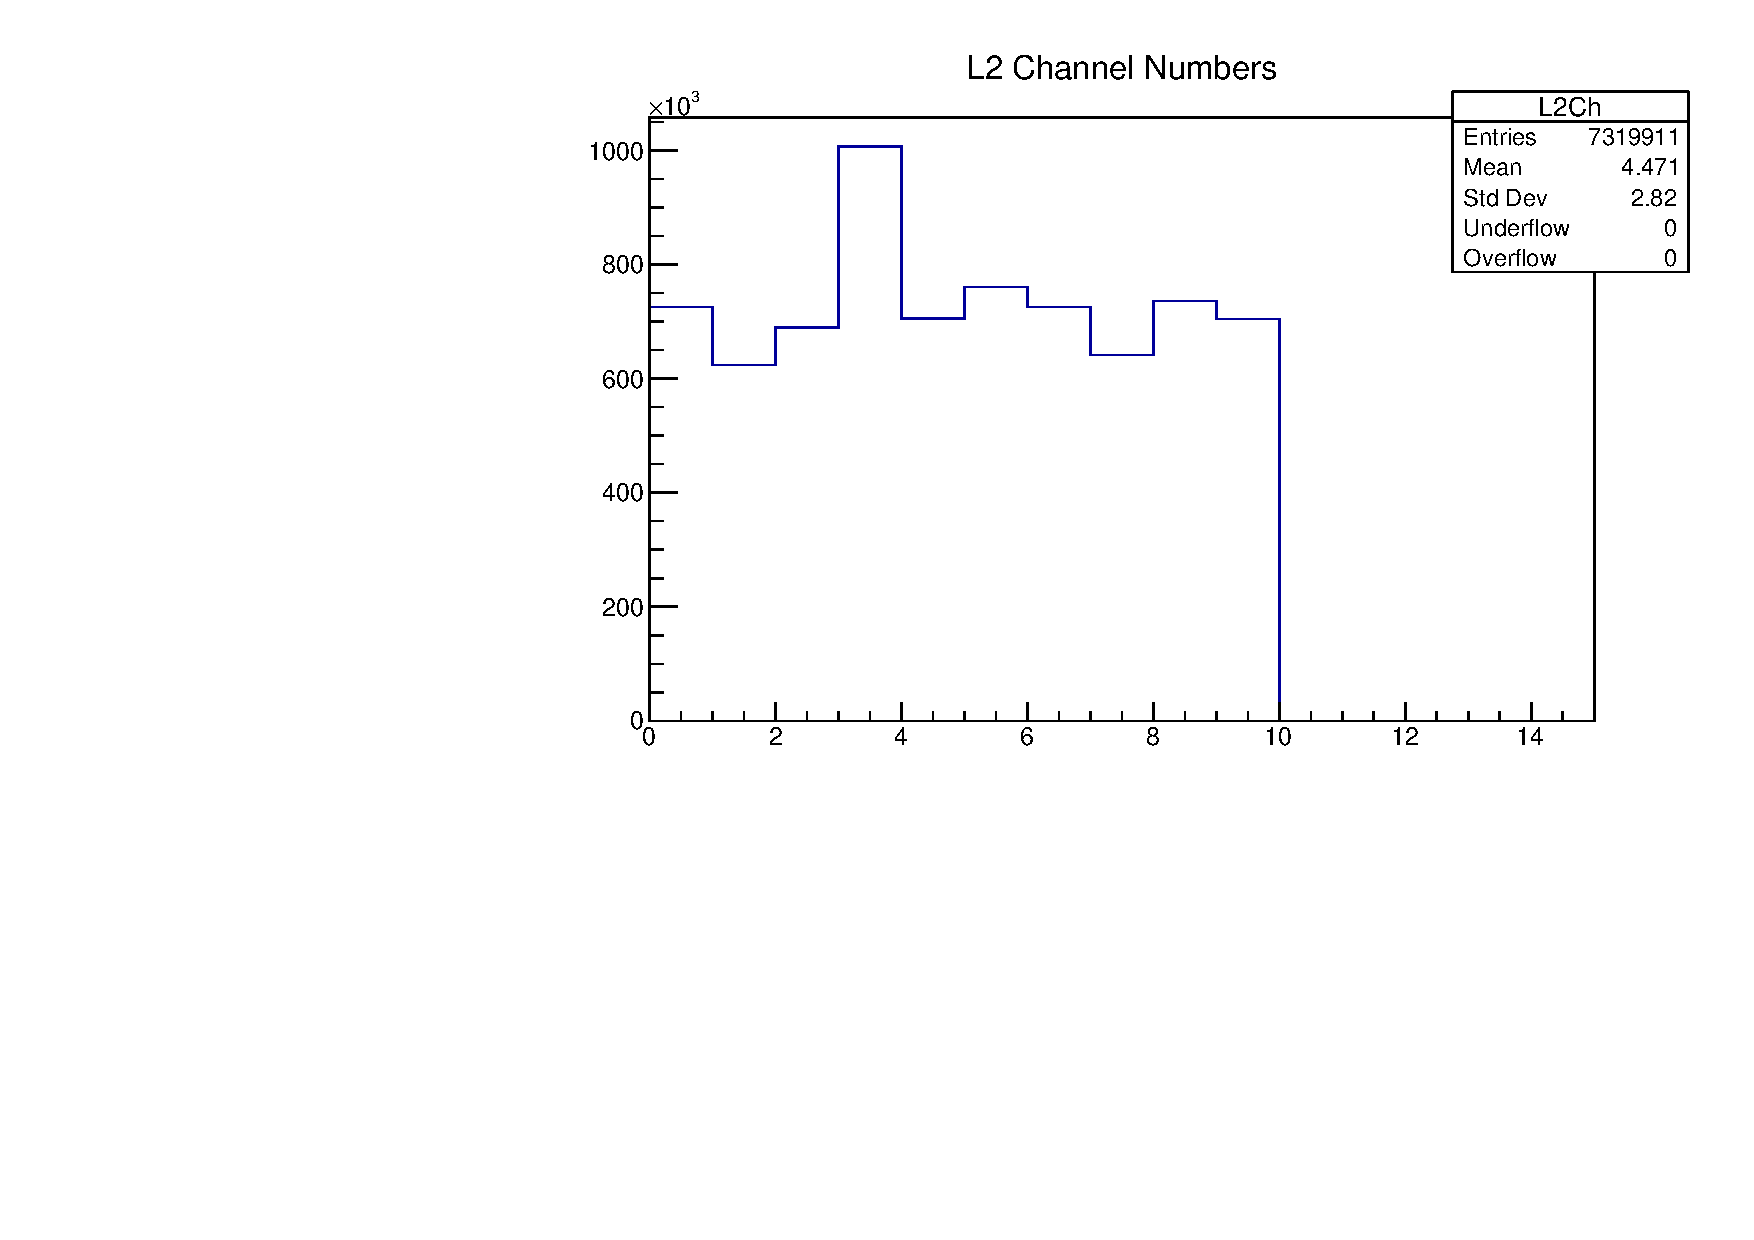
\includegraphics[width=0.33\textwidth,scale=0.5,trim=0 0 0 0,clip]{plotsdir/file0_test-L2Ch-1.pdf} 
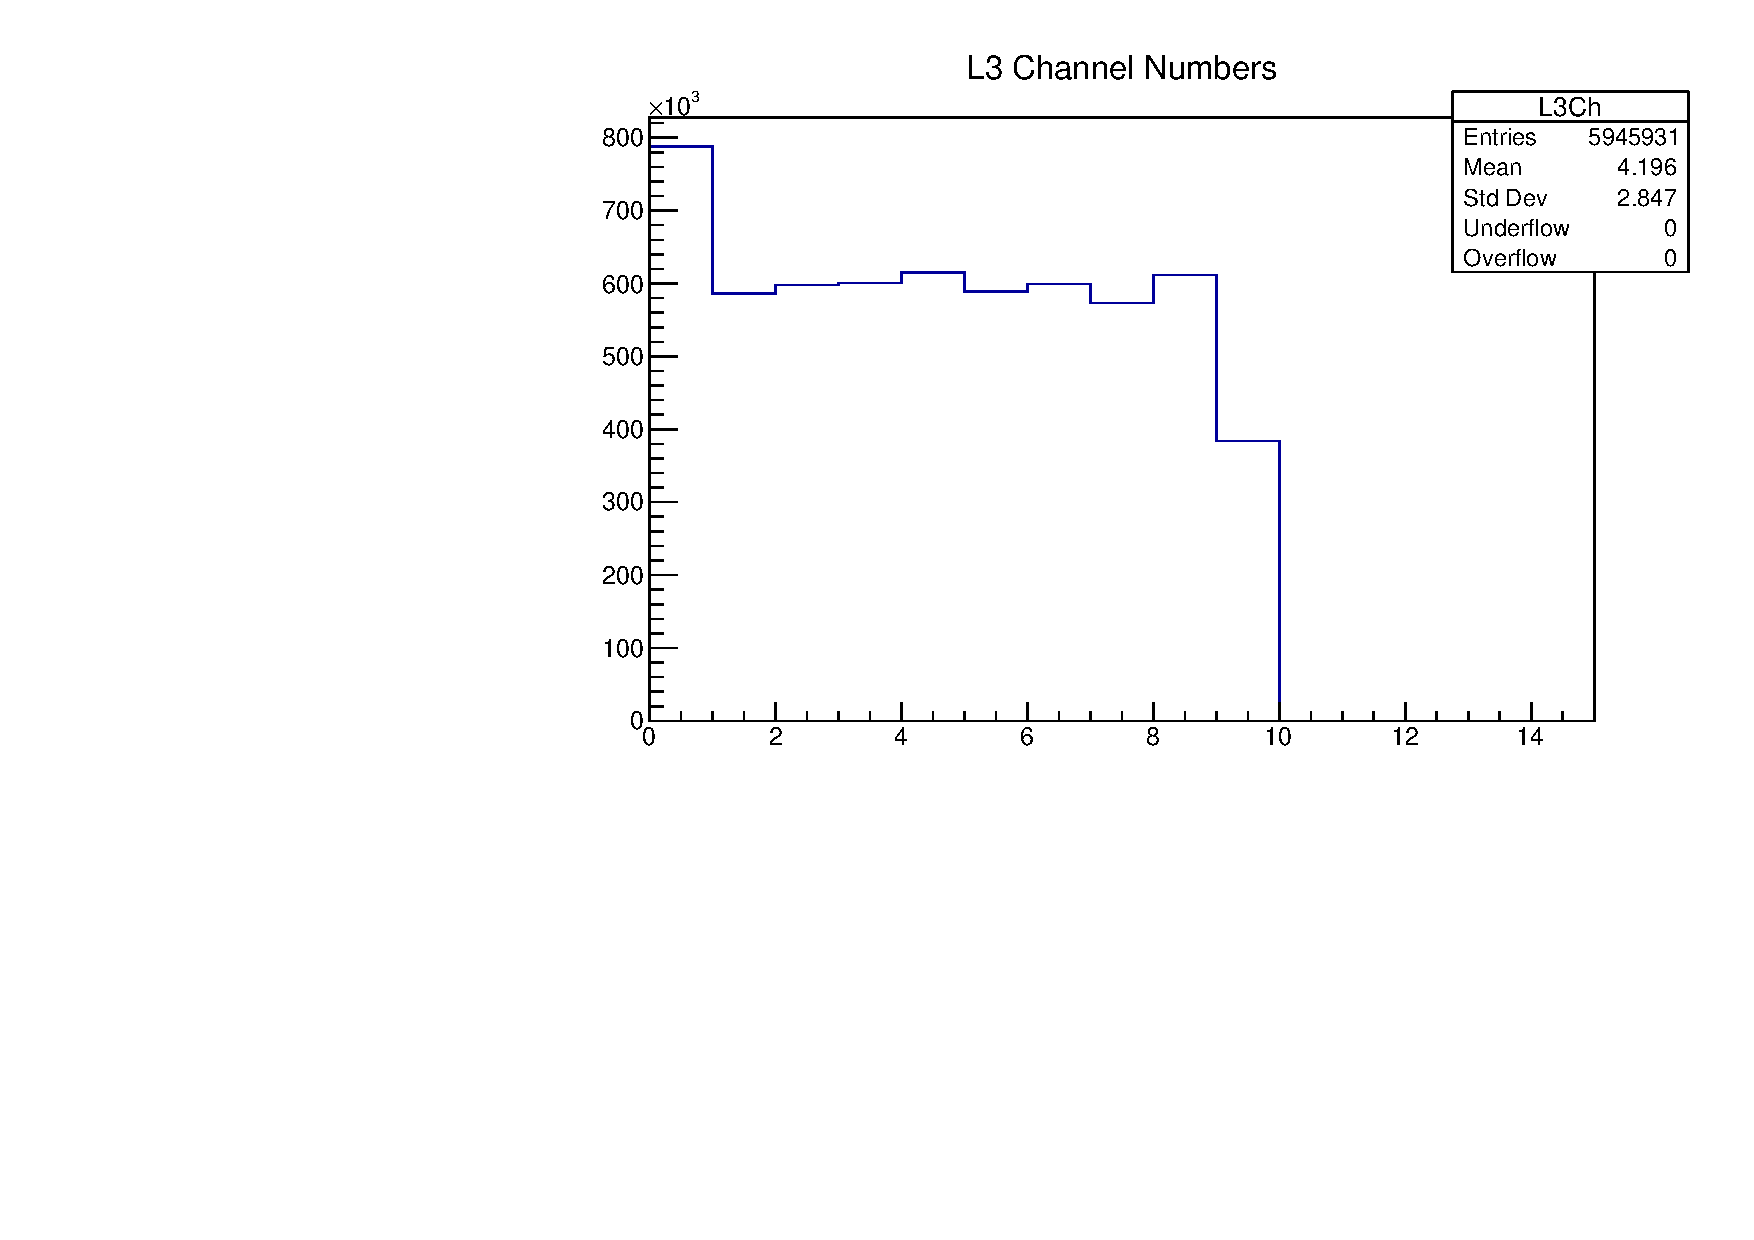
\includegraphics[width=0.33\textwidth,scale=0.5,trim=0 0 0 0,clip]{plotsdir/file0_test-L3Ch-1.pdf} 
\caption{(a)L1 Channel Numbers ~~~(b) L2 Channel Numbers ~~~(c)L3 Channel Numbers } 
\end{figure} 
\begin{figure}[H] 
\vspace*{-0.3cm} 
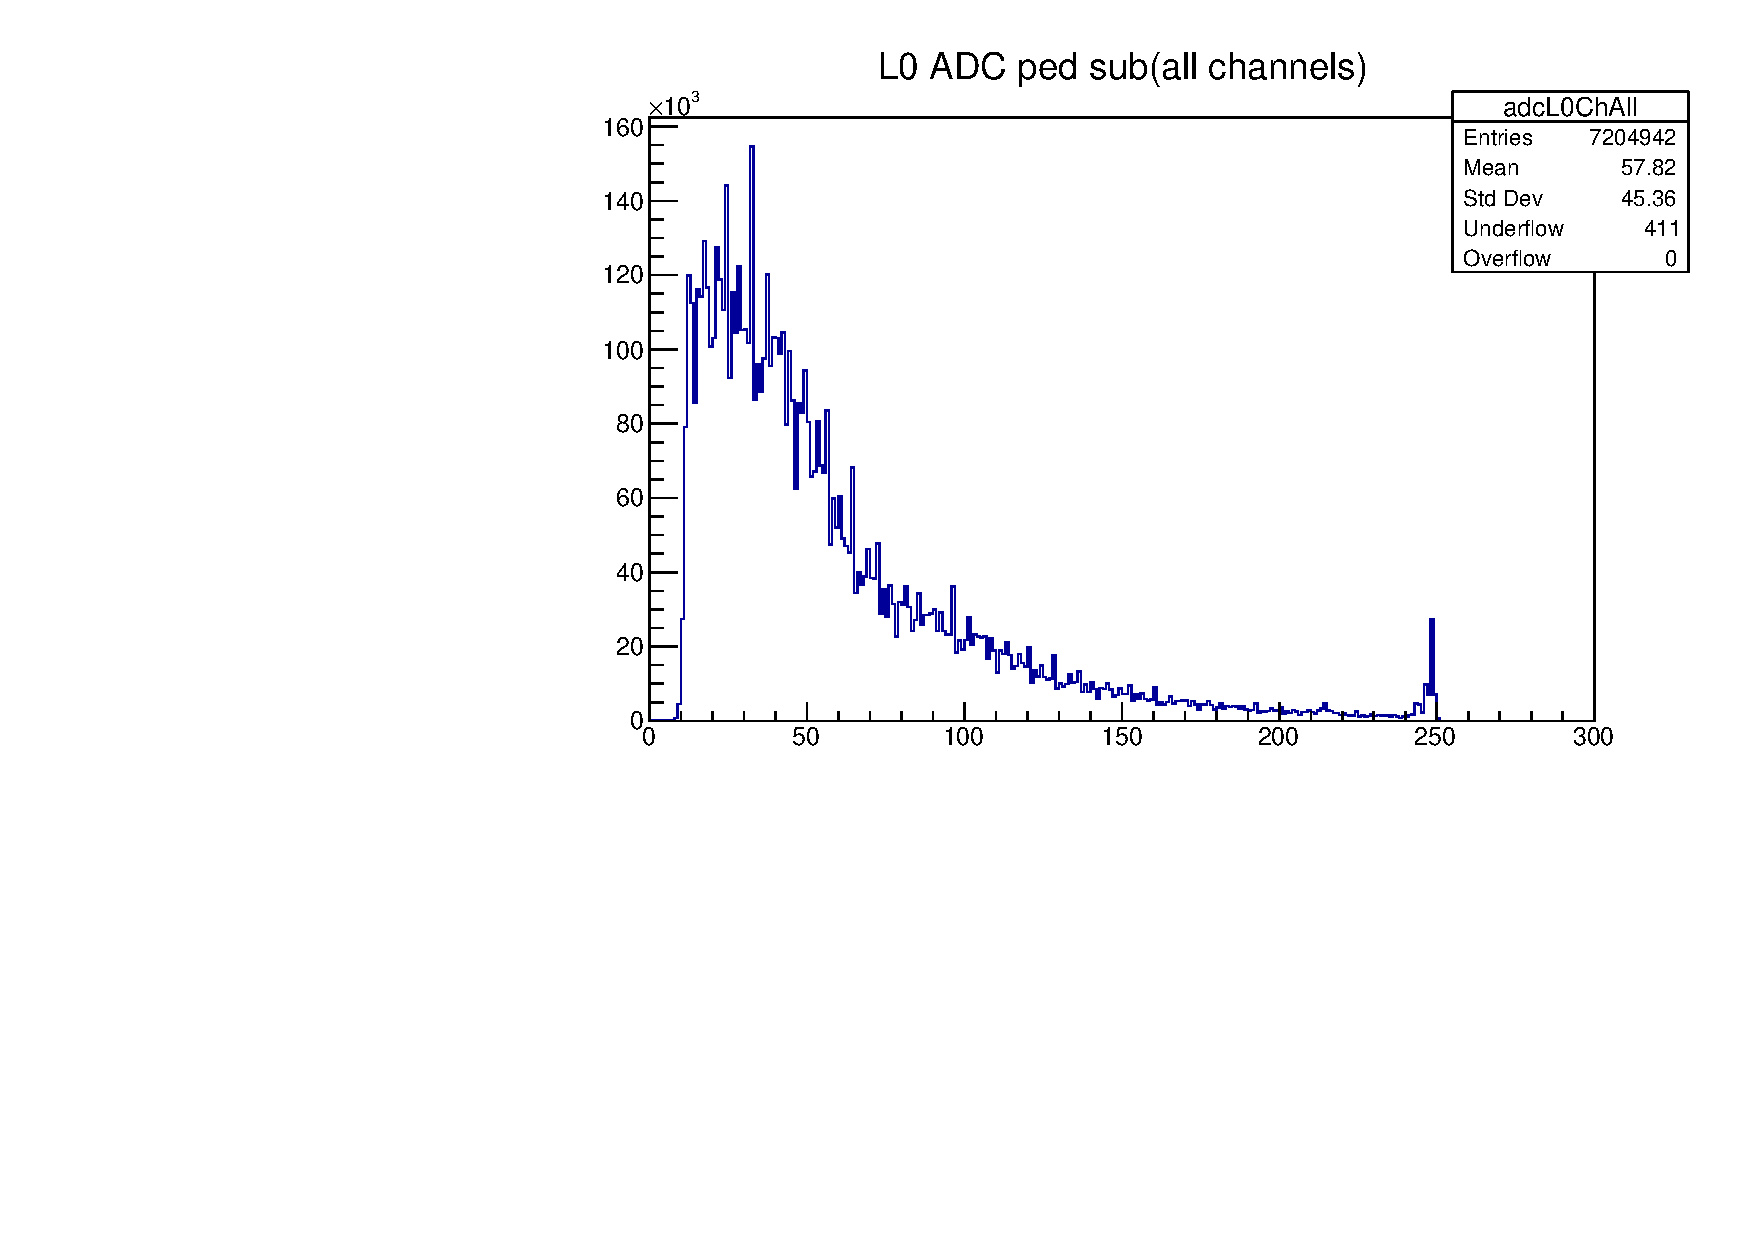
\includegraphics[width=0.33\textwidth,scale=0.5,trim=0 0 0 0,clip]{plotsdir/file0_test-adcL0ChAll-1.pdf} 
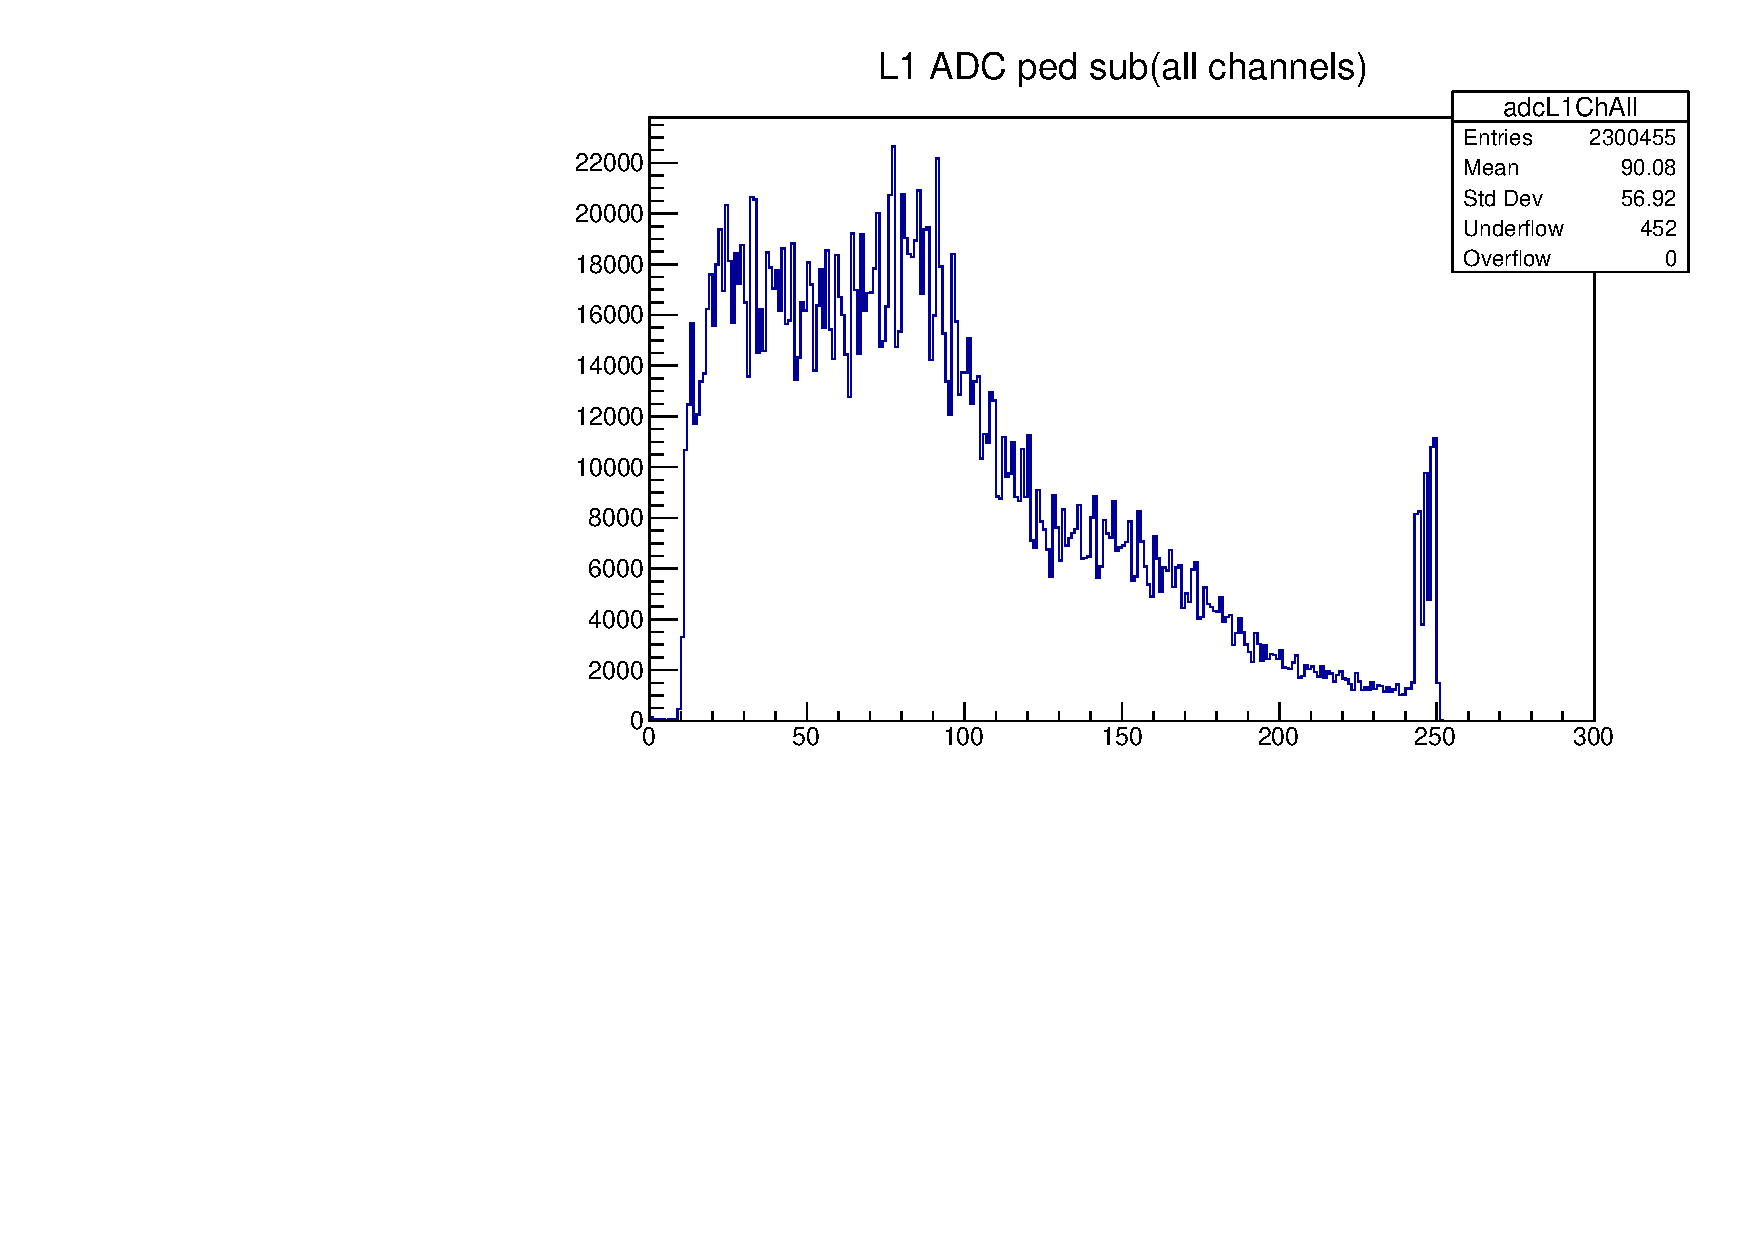
\includegraphics[width=0.33\textwidth,scale=0.5,trim=0 0 0 0,clip]{plotsdir/file0_test-adcL1ChAll-1.pdf} 
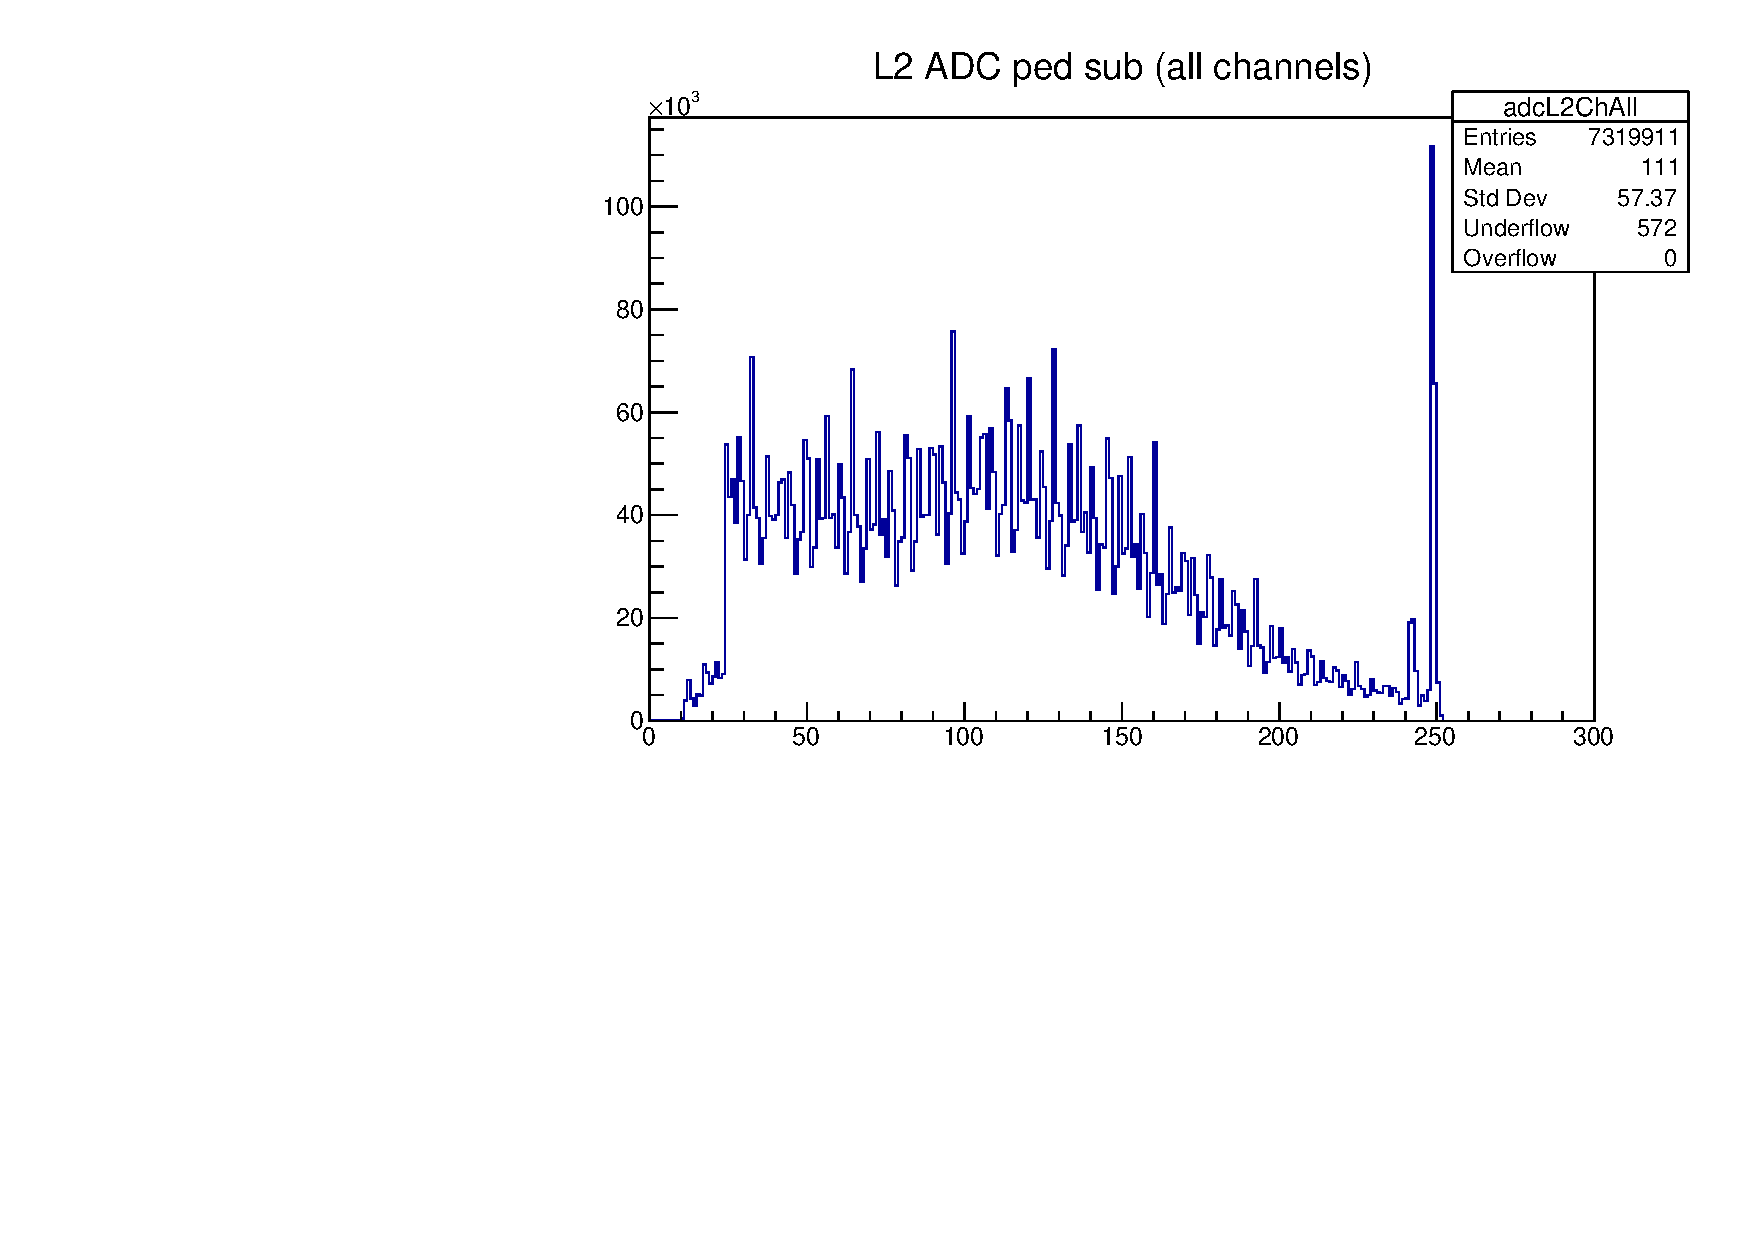
\includegraphics[width=0.33\textwidth,scale=0.5,trim=0 0 0 0,clip]{plotsdir/file0_test-adcL2ChAll-1.pdf} 
\caption{(a)L0 ADC ped sub(all channels) ~~~(b) L1 ADC ped sub(all channels) ~~~(c)L2 ADC ped sub (all channels) } 
\end{figure} 
\begin{figure}[H] 
\vspace*{-0.3cm} 
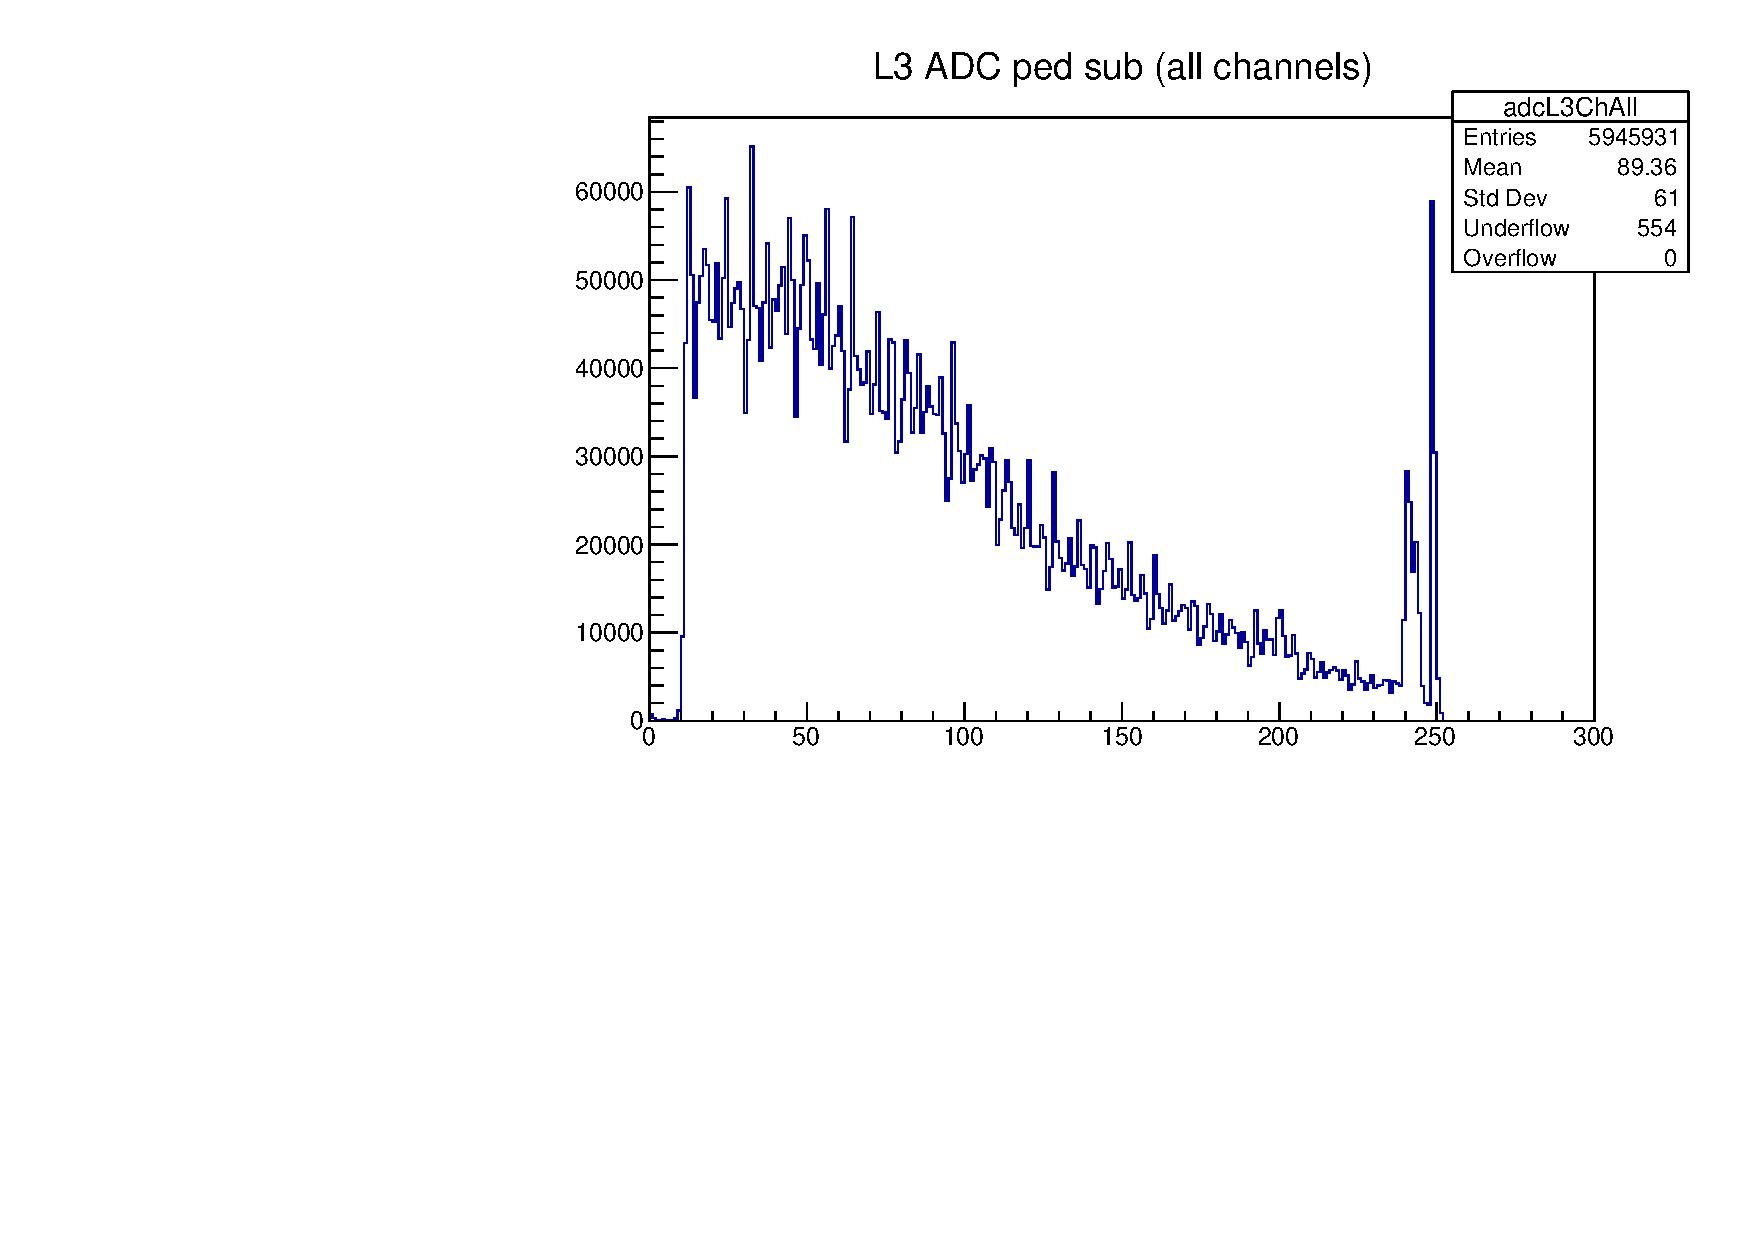
\includegraphics[width=0.33\textwidth,scale=0.5,trim=0 0 0 0,clip]{plotsdir/file0_test-adcL3ChAll-1.pdf} 
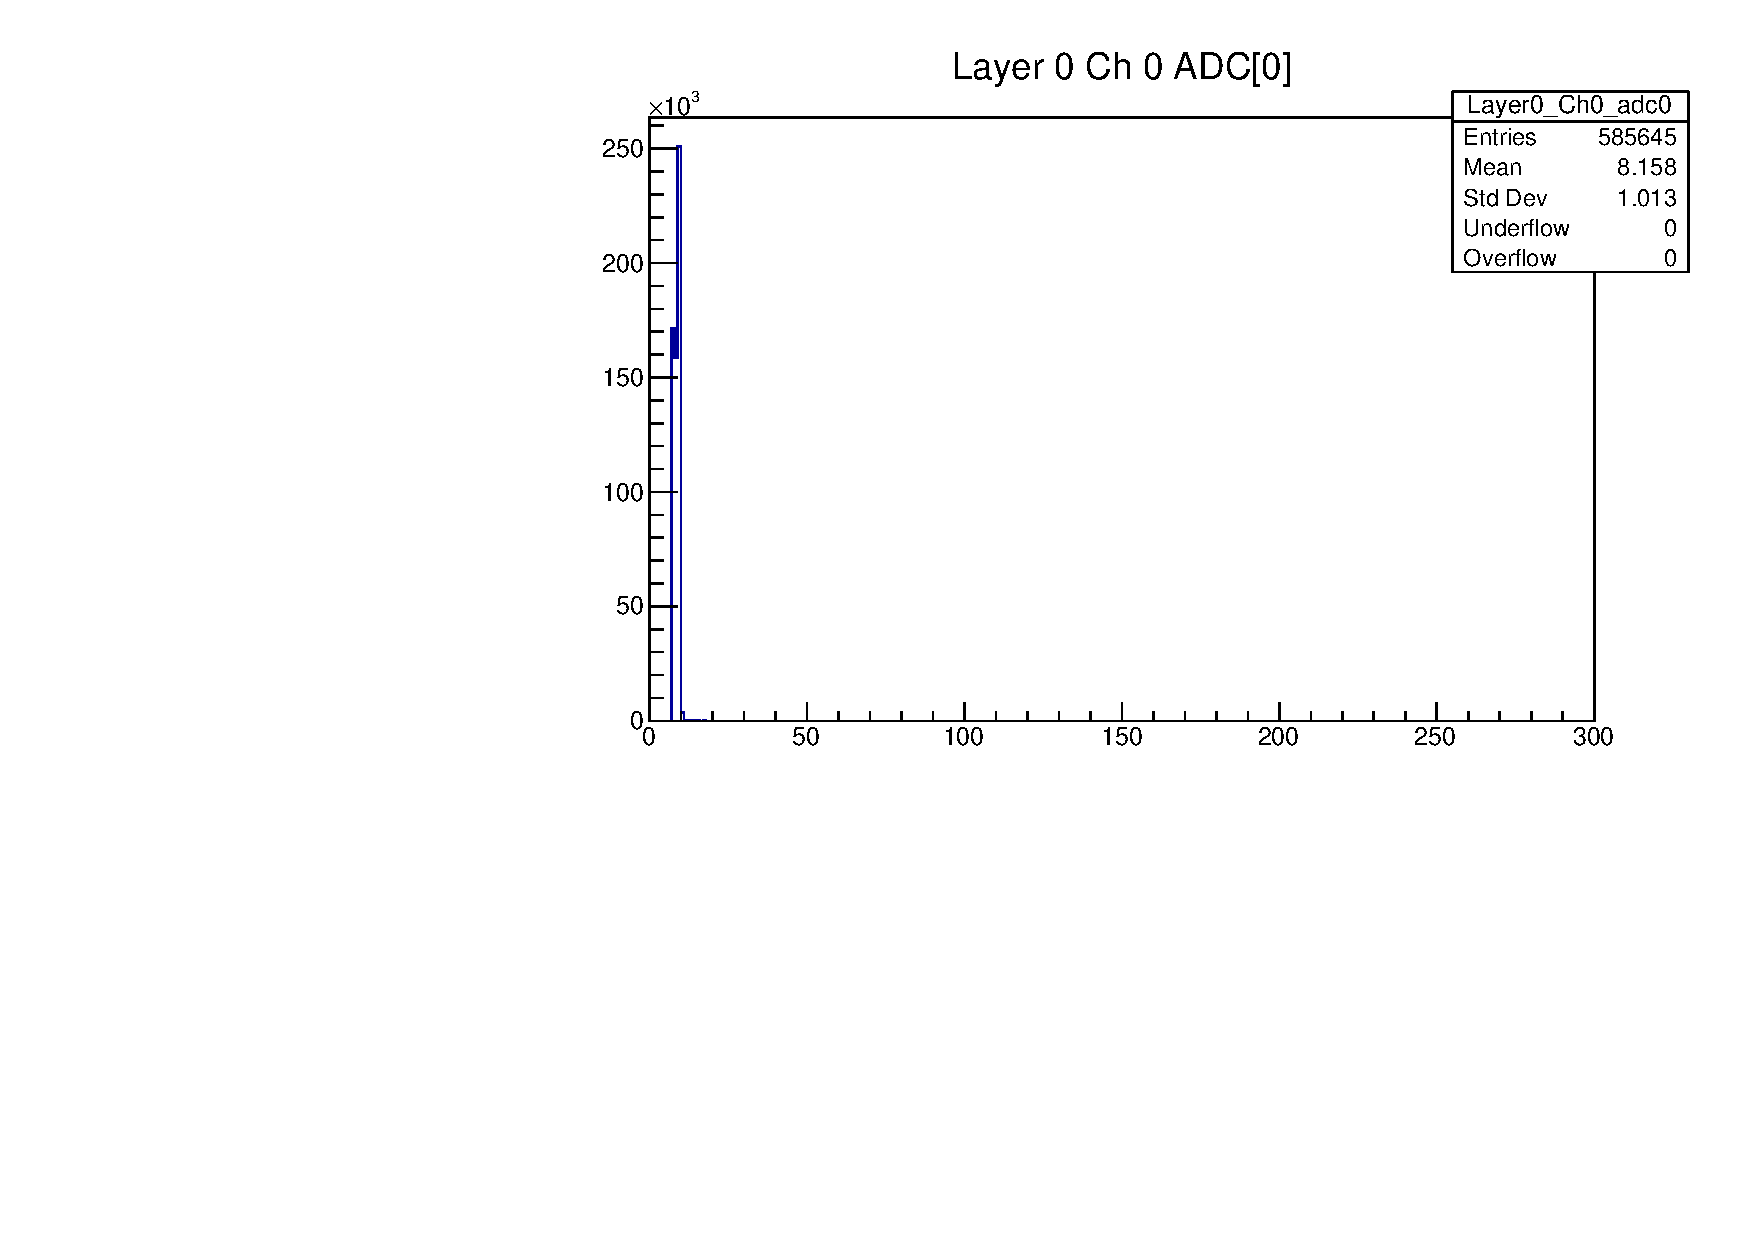
\includegraphics[width=0.33\textwidth,scale=0.5,trim=0 0 0 0,clip]{plotsdir/file0_test-Layer0_Ch0_adc0-1.pdf} 
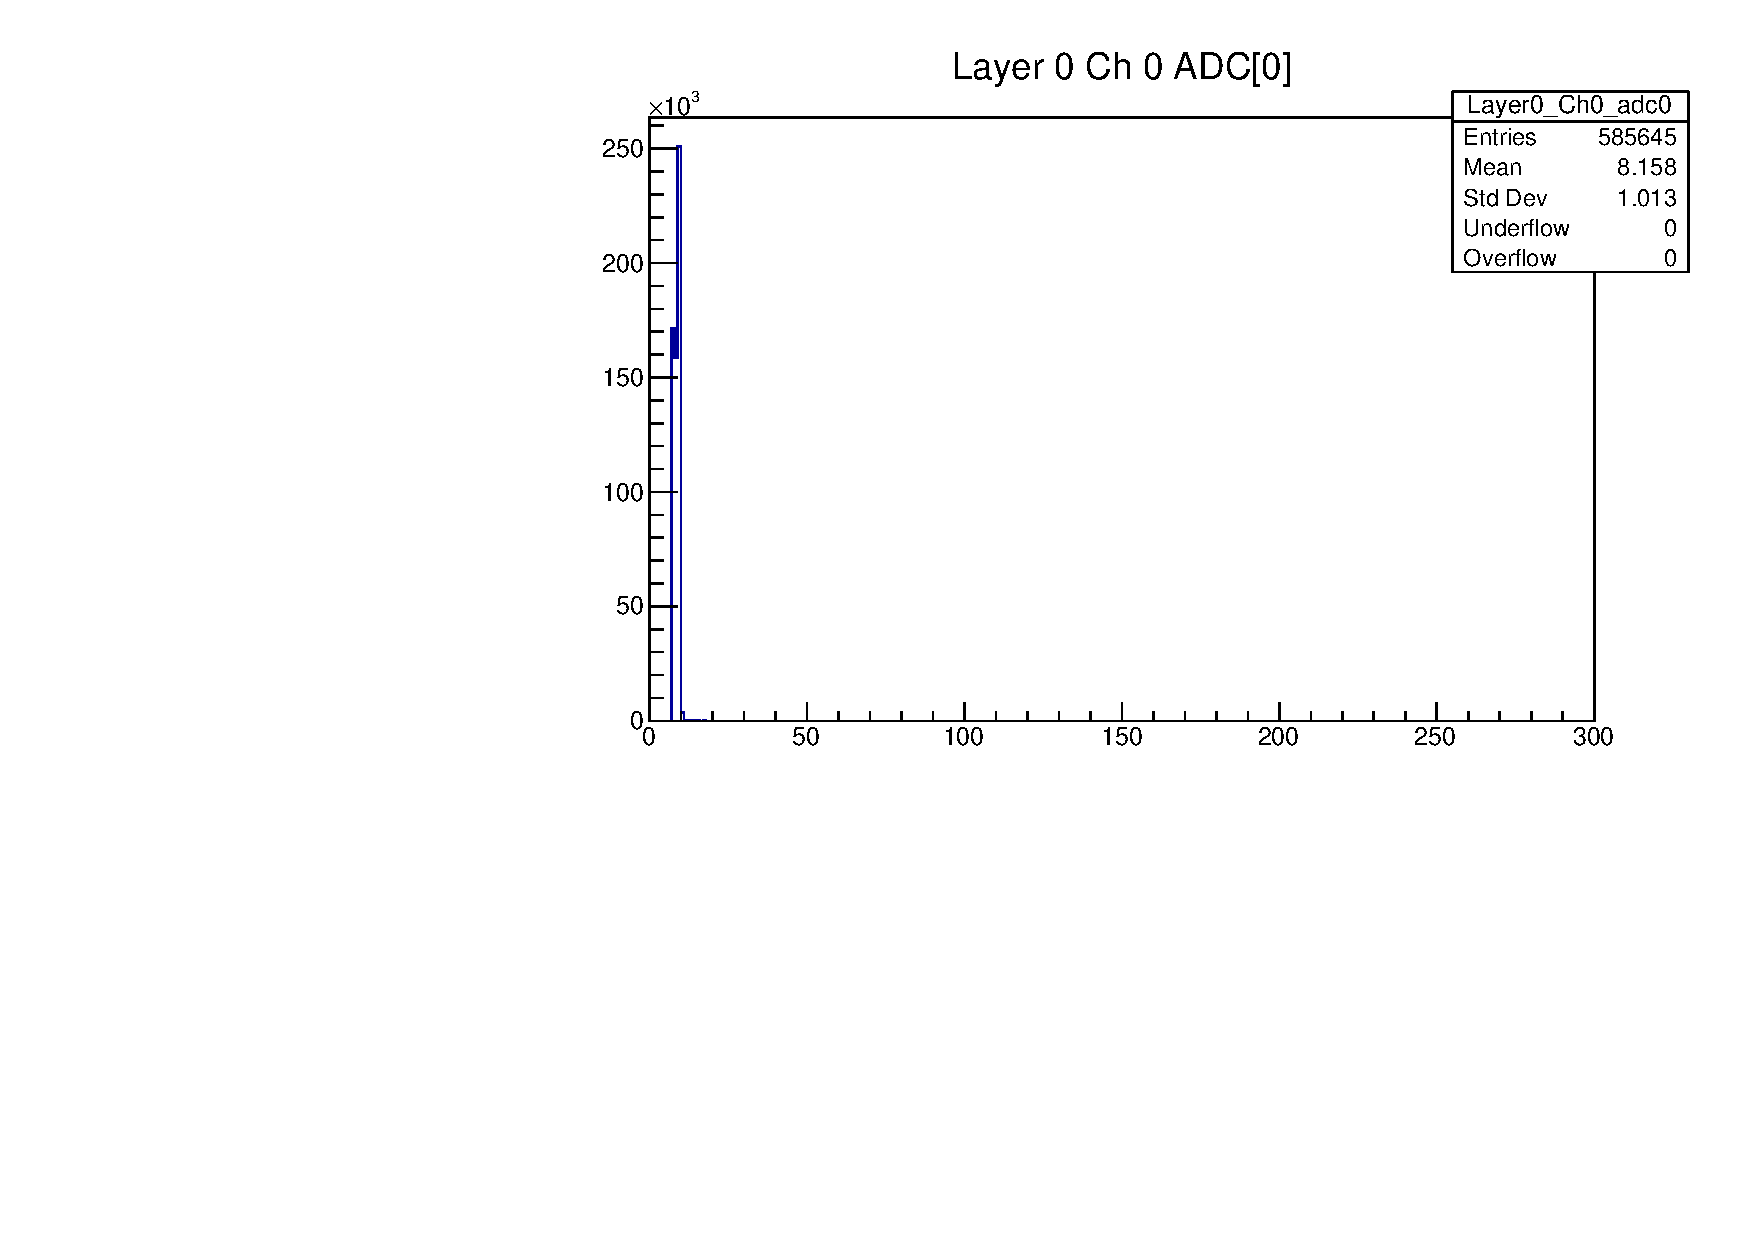
\includegraphics[width=0.33\textwidth,scale=0.5,trim=0 0 0 0,clip]{plotsdir/file0_test-Layer0_Ch0_adc0-1.pdf} 
\caption{(a)L3 ADC ped sub (all channels) ~~~(b) Layer 0 Ch 0 ADC[0] ~~~(c)Layer 0 Ch 0 ADC[0] } 
\end{figure} 
\begin{figure}[H] 
\vspace*{-0.3cm} 
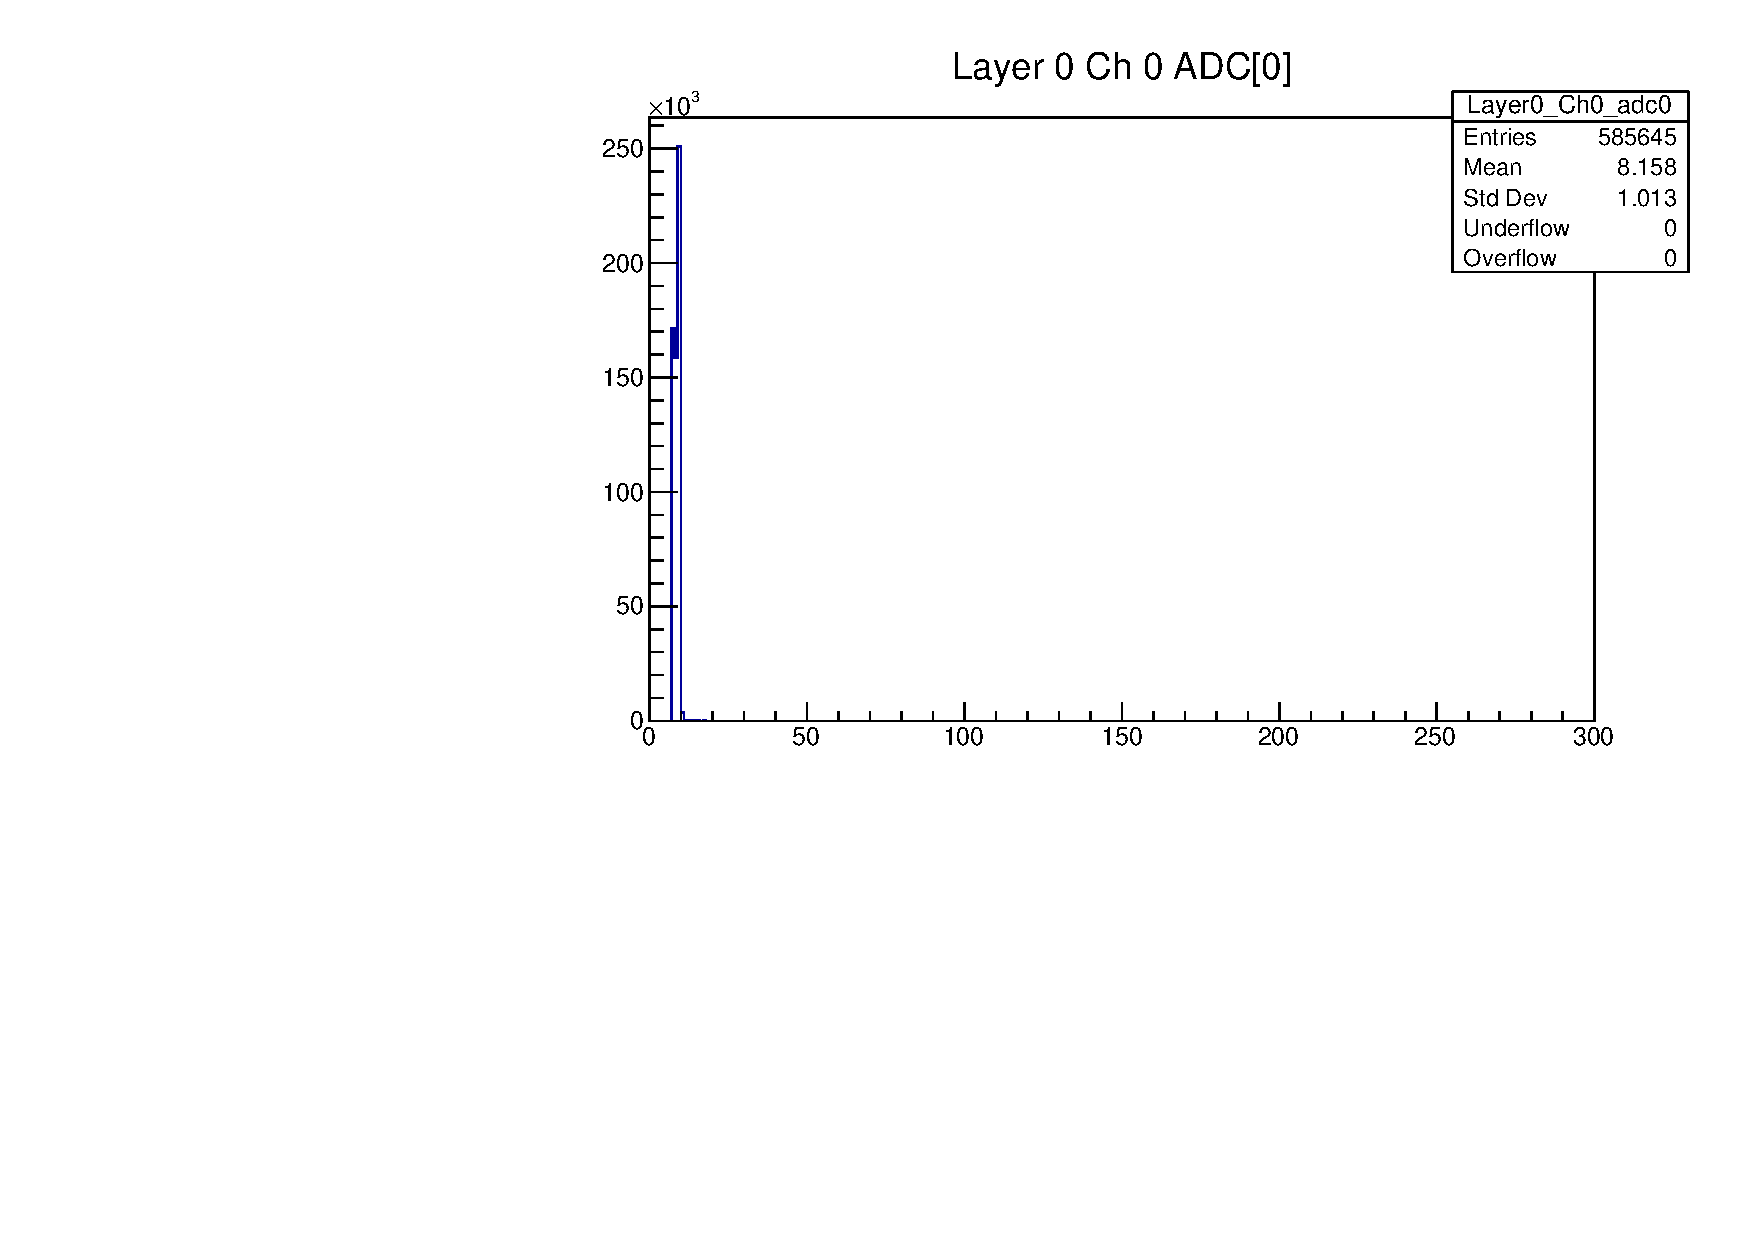
\includegraphics[width=0.33\textwidth,scale=0.5,trim=0 0 0 0,clip]{plotsdir/file0_test-Layer0_Ch0_adc0-1.pdf} 
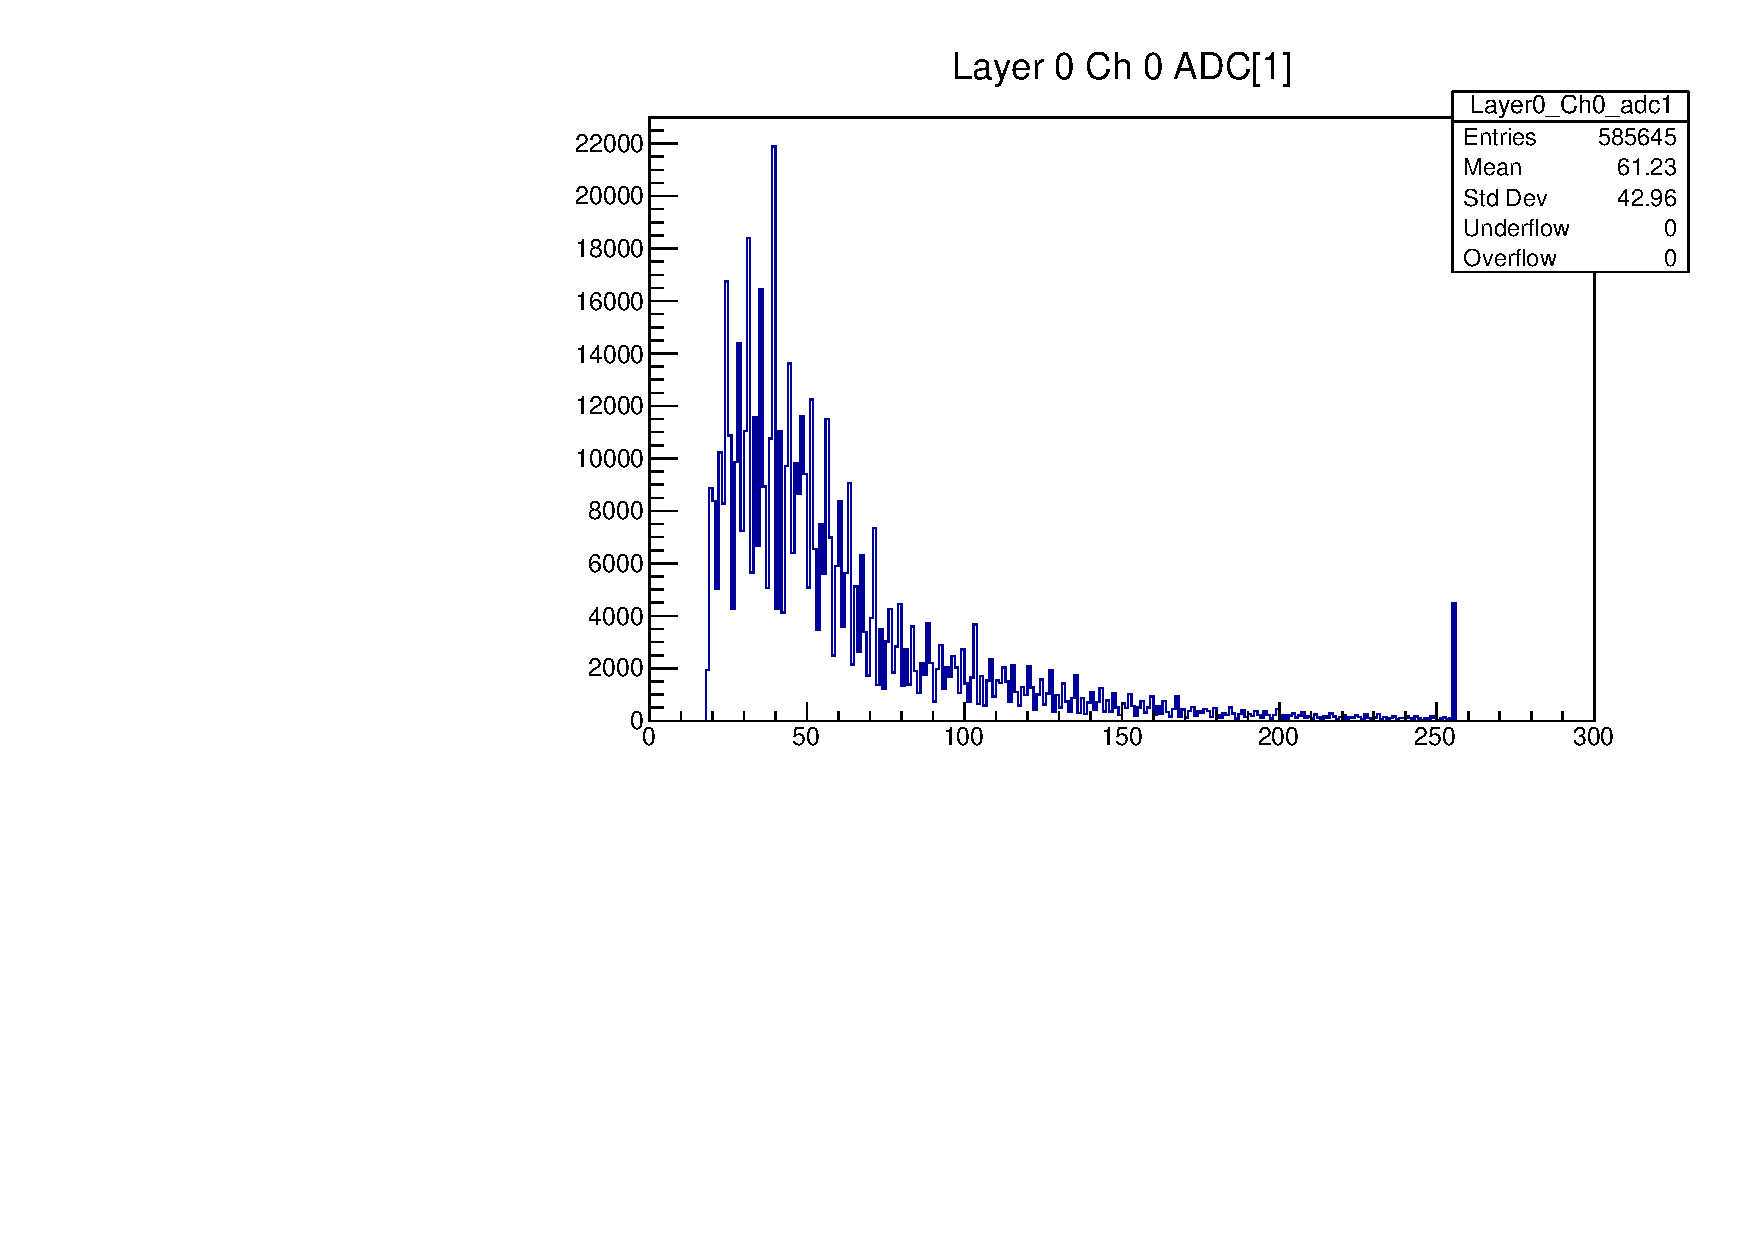
\includegraphics[width=0.33\textwidth,scale=0.5,trim=0 0 0 0,clip]{plotsdir/file0_test-Layer0_Ch0_adc1-1.pdf} 
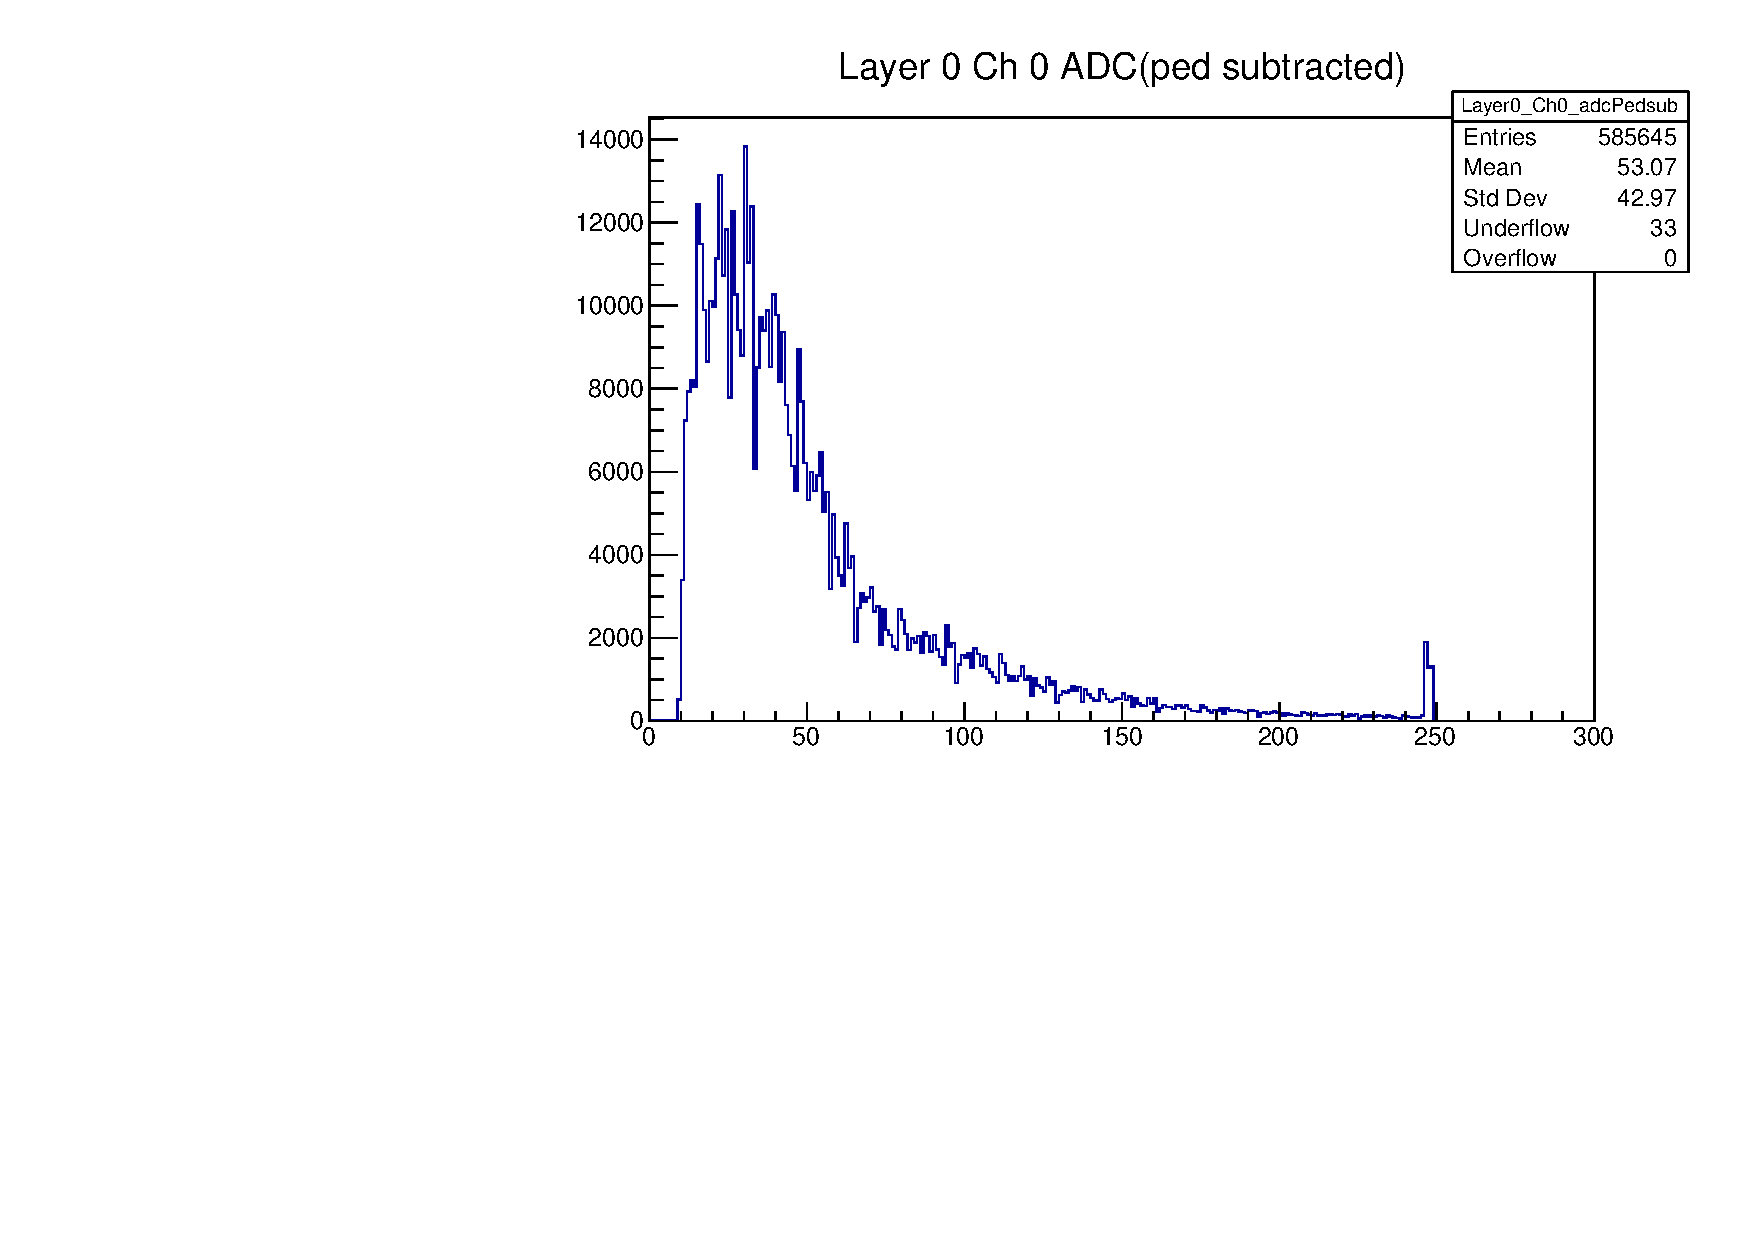
\includegraphics[width=0.33\textwidth,scale=0.5,trim=0 0 0 0,clip]{plotsdir/file0_test-Layer0_Ch0_adcPedsub-1.pdf} 
\caption{(a)Layer 0 Ch 0 ADC[0] ~~~(b) Layer 0 Ch 0 ADC[1] ~~~(c)Layer 0 Ch 0 ADC(ped subtracted) } 
\end{figure} 
\begin{figure}[H] 
\vspace*{-0.3cm} 
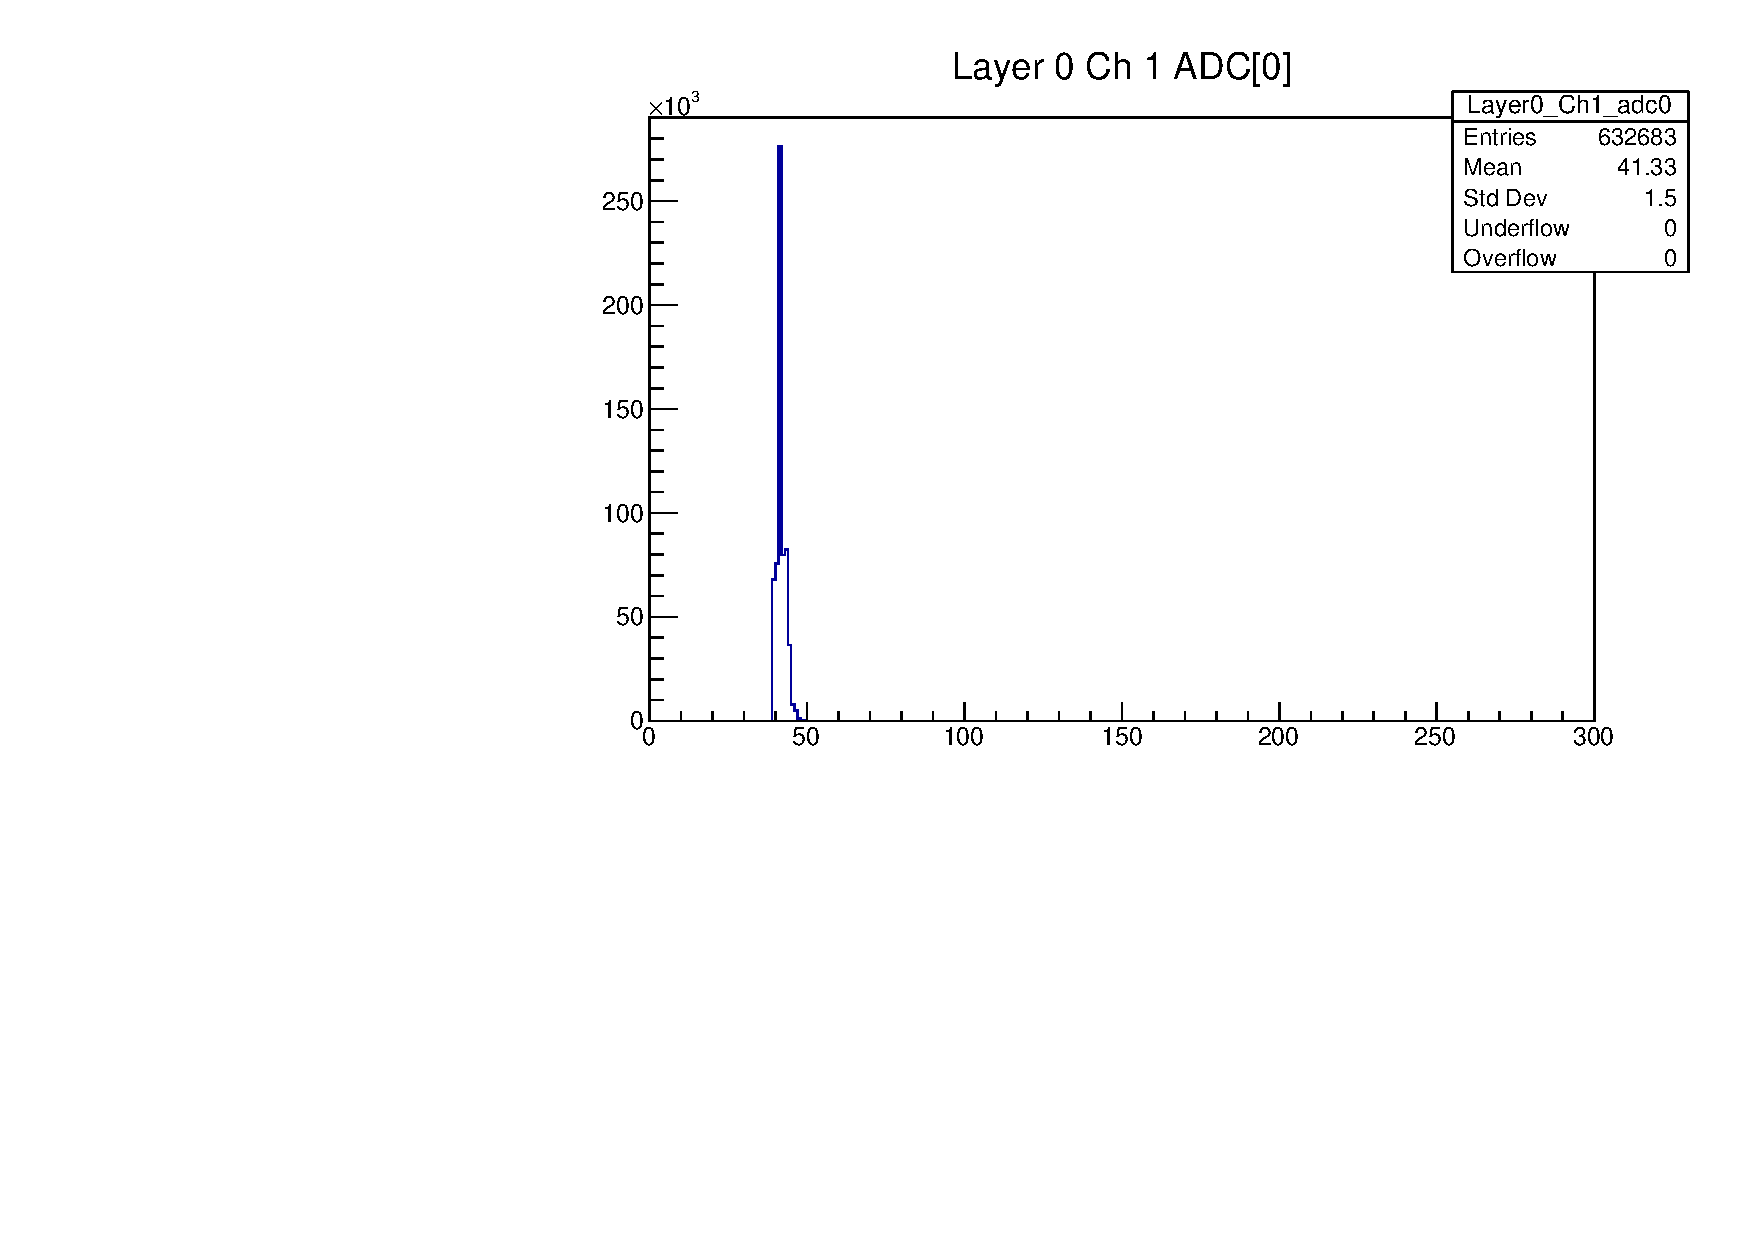
\includegraphics[width=0.33\textwidth,scale=0.5,trim=0 0 0 0,clip]{plotsdir/file0_test-Layer0_Ch1_adc0-1.pdf} 
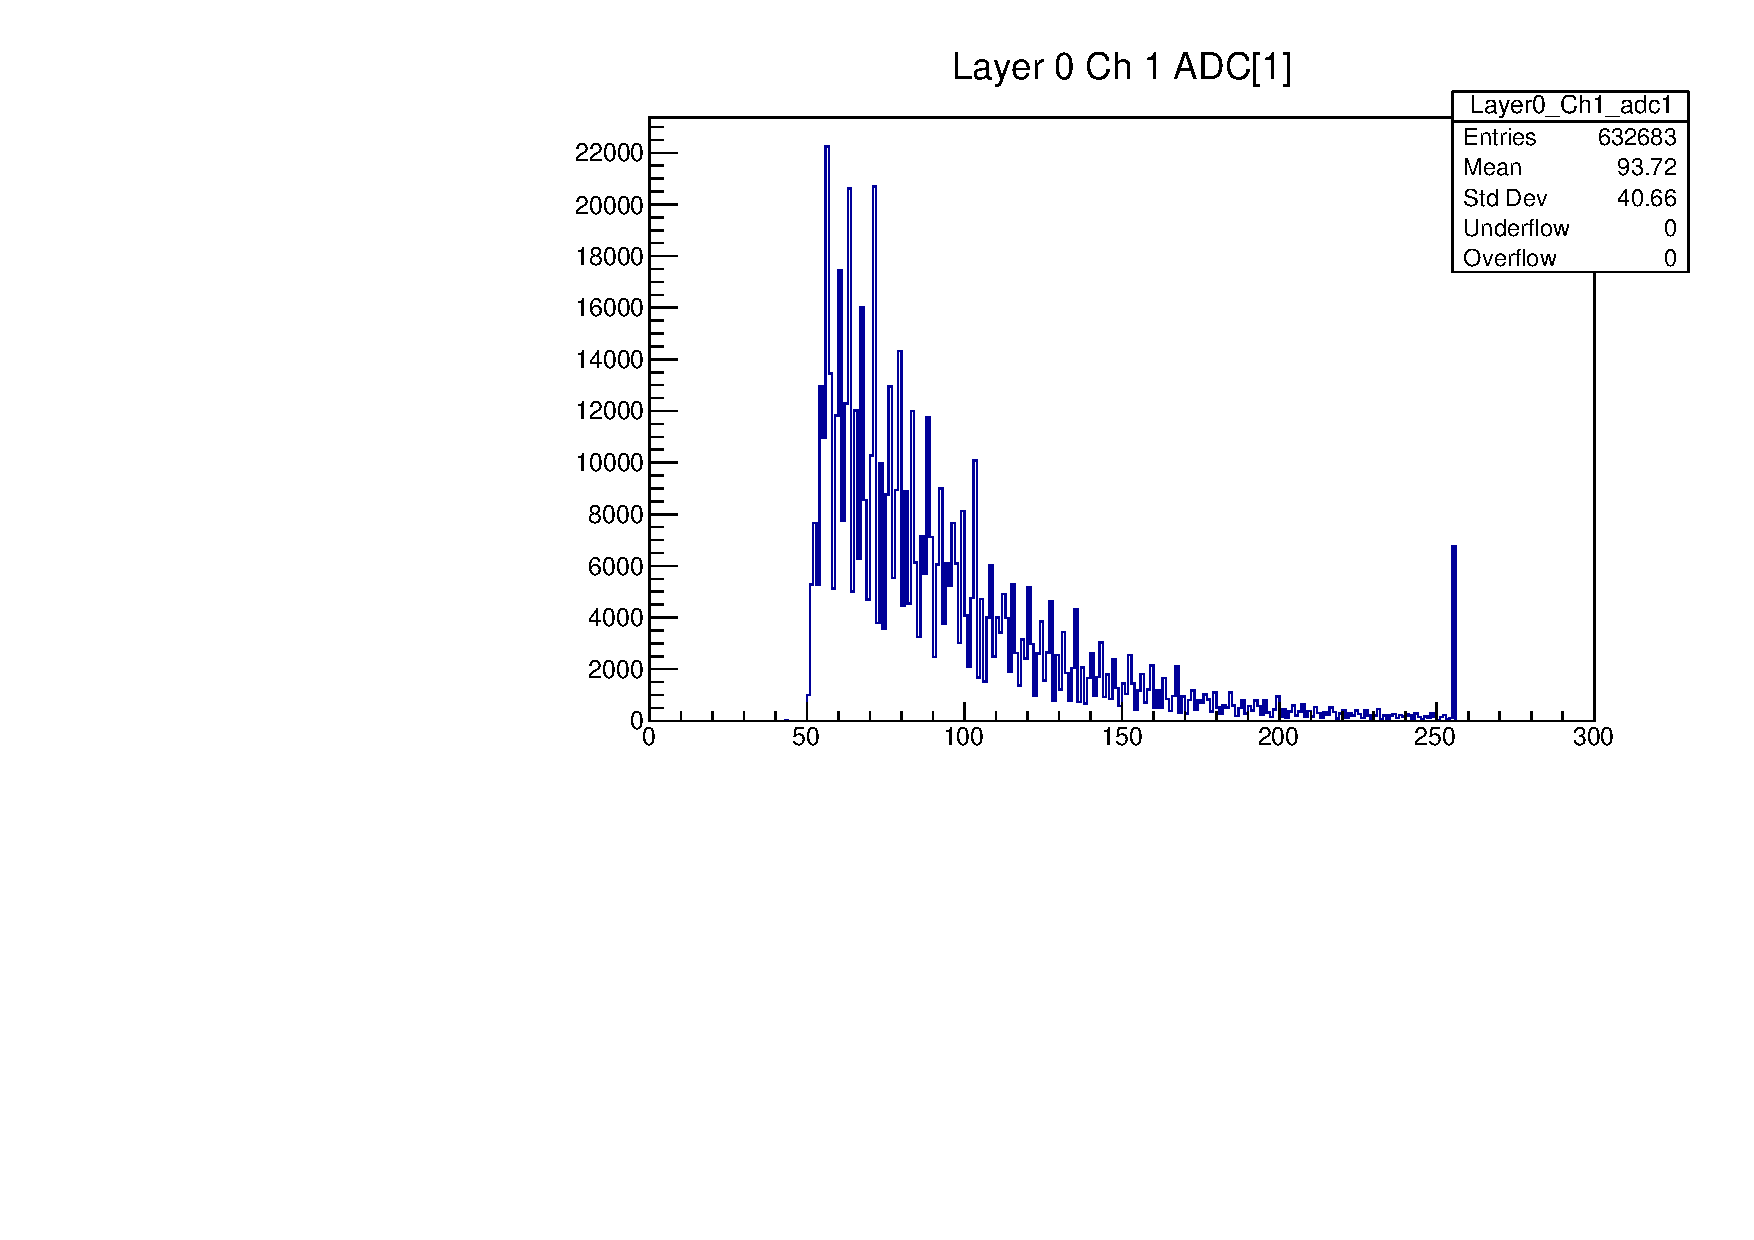
\includegraphics[width=0.33\textwidth,scale=0.5,trim=0 0 0 0,clip]{plotsdir/file0_test-Layer0_Ch1_adc1-1.pdf} 
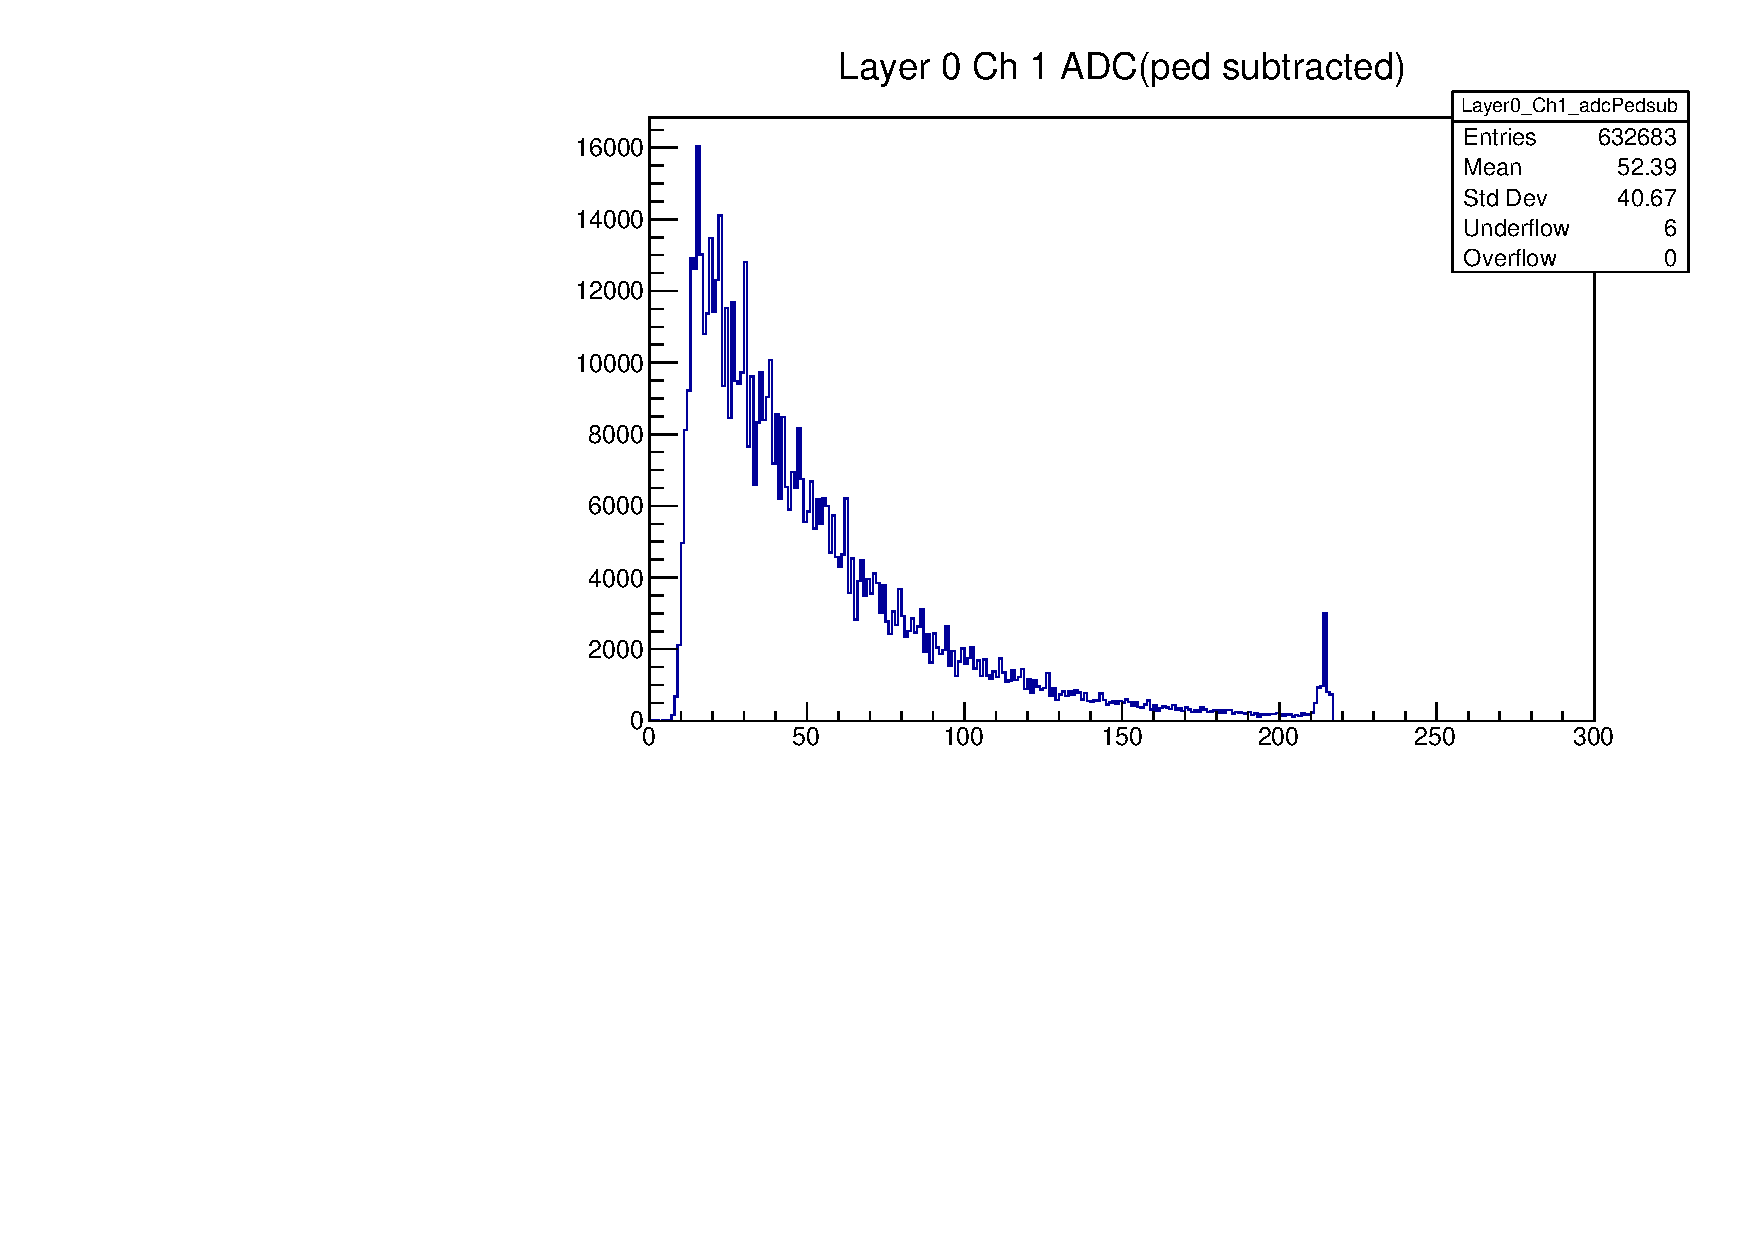
\includegraphics[width=0.33\textwidth,scale=0.5,trim=0 0 0 0,clip]{plotsdir/file0_test-Layer0_Ch1_adcPedsub-1.pdf} 
\caption{(a)Layer 0 Ch 1 ADC[0] ~~~(b) Layer 0 Ch 1 ADC[1] ~~~(c)Layer 0 Ch 1 ADC(ped subtracted) } 
\end{figure} 
\clearpage 
\begin{figure}[H] 
\vspace*{-0.3cm} 
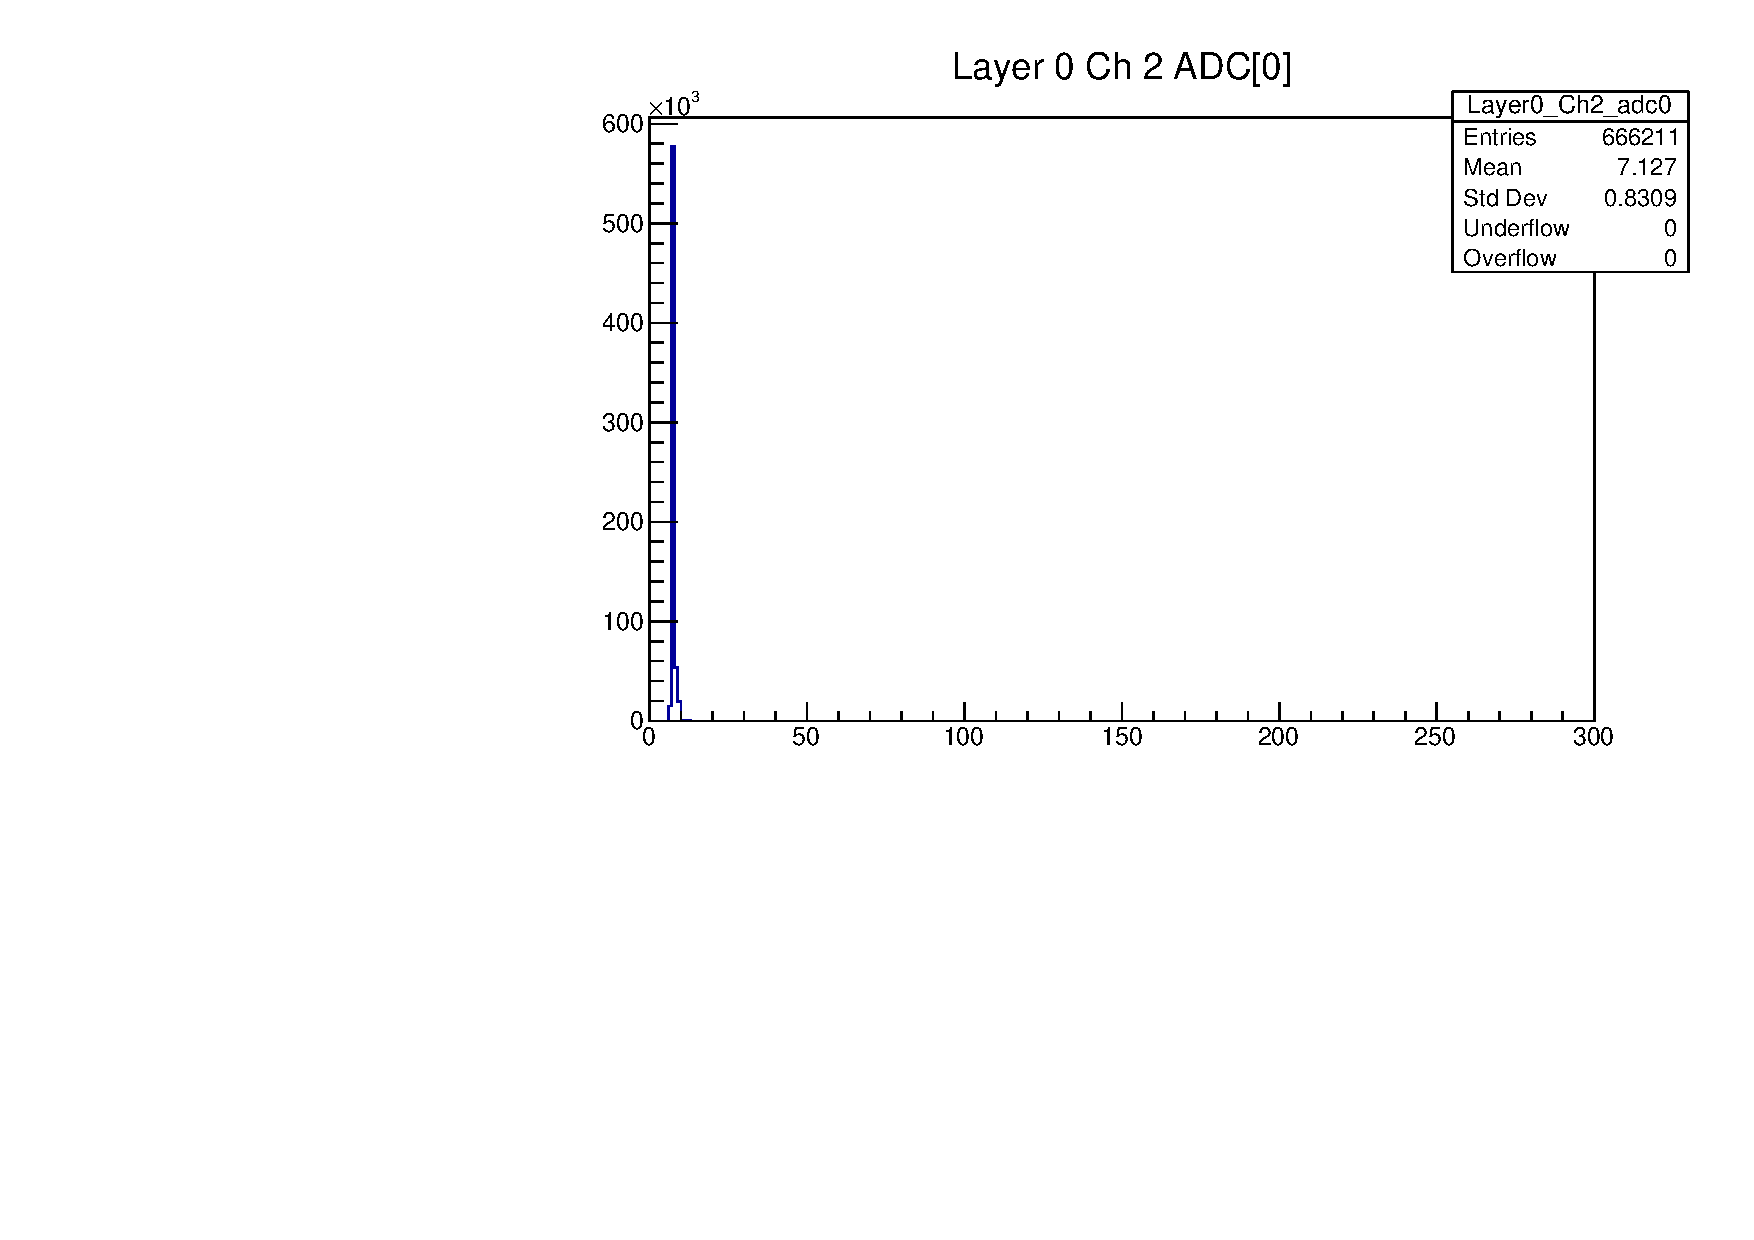
\includegraphics[width=0.33\textwidth,scale=0.5,trim=0 0 0 0,clip]{plotsdir/file0_test-Layer0_Ch2_adc0-1.pdf} 
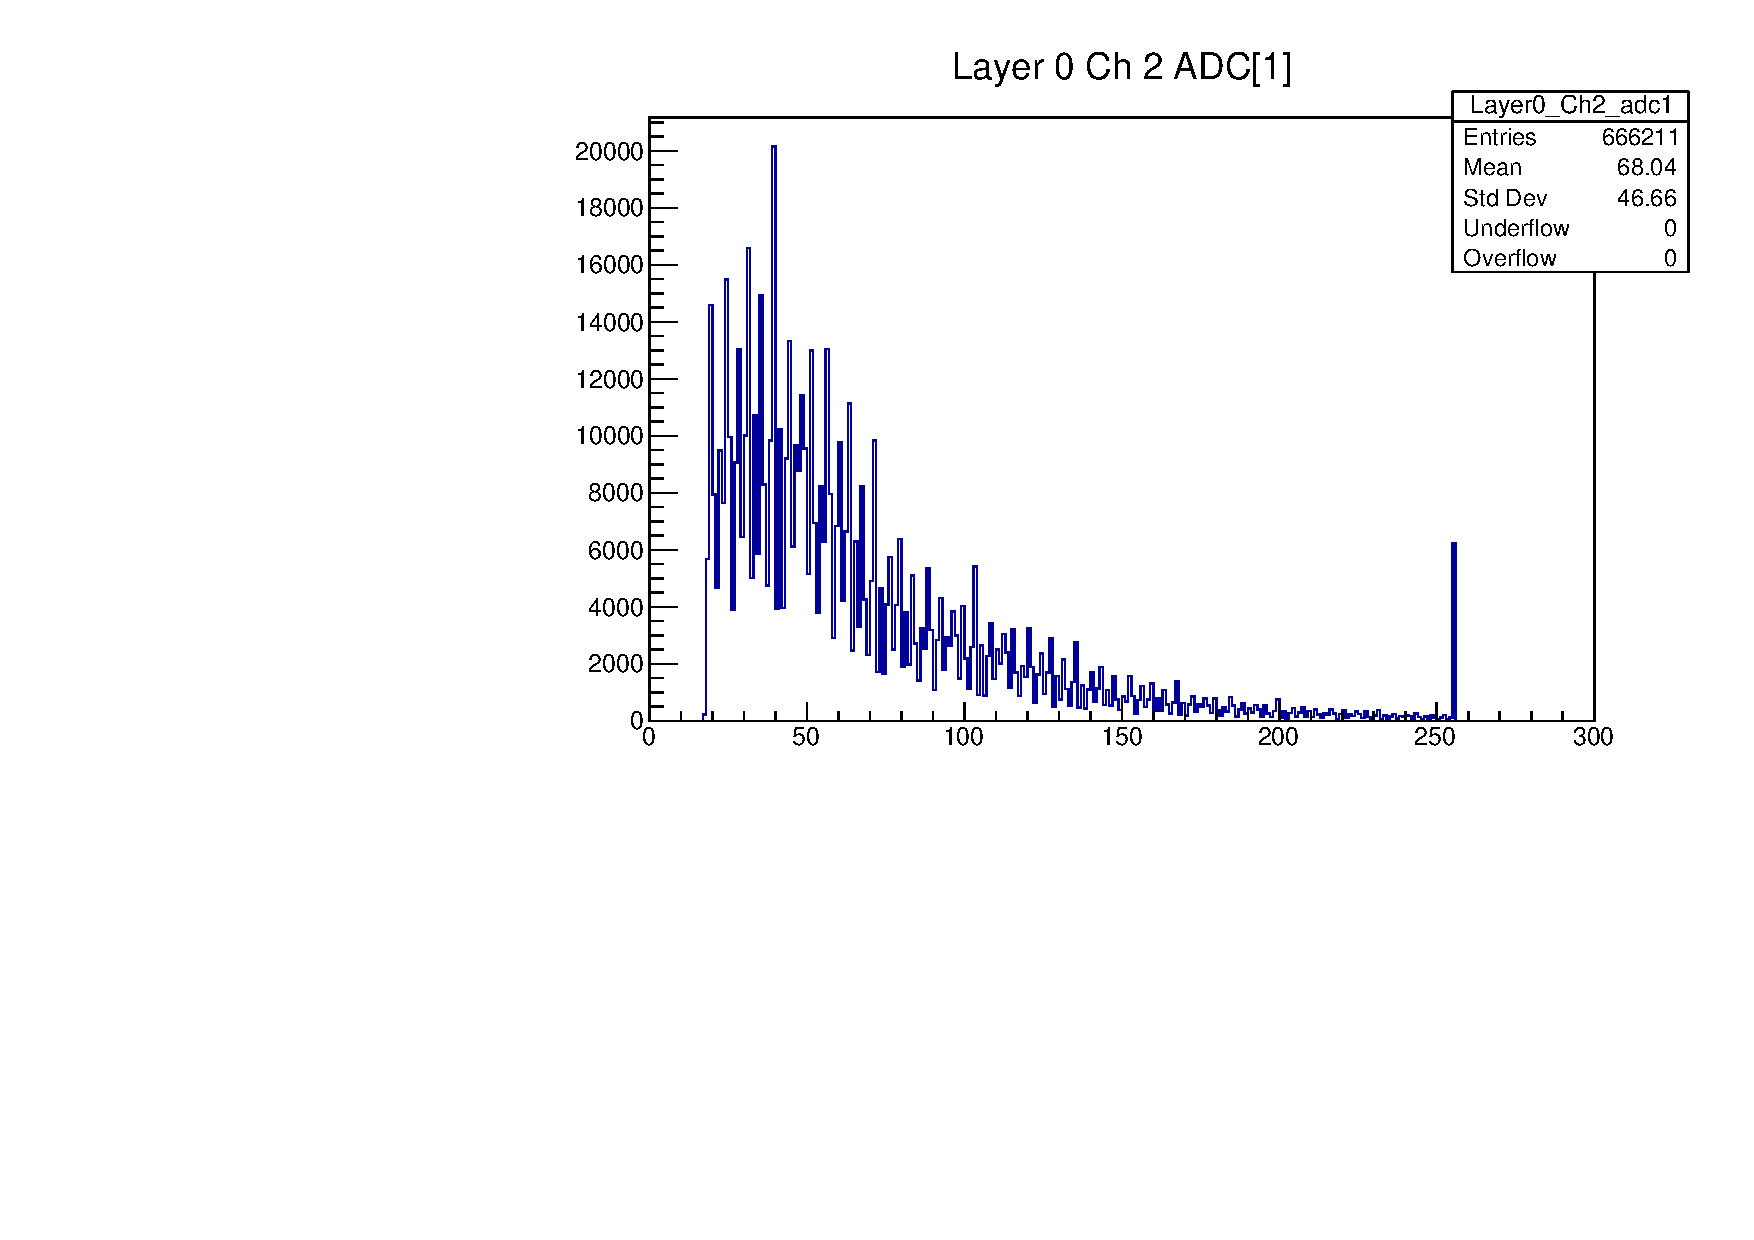
\includegraphics[width=0.33\textwidth,scale=0.5,trim=0 0 0 0,clip]{plotsdir/file0_test-Layer0_Ch2_adc1-1.pdf} 
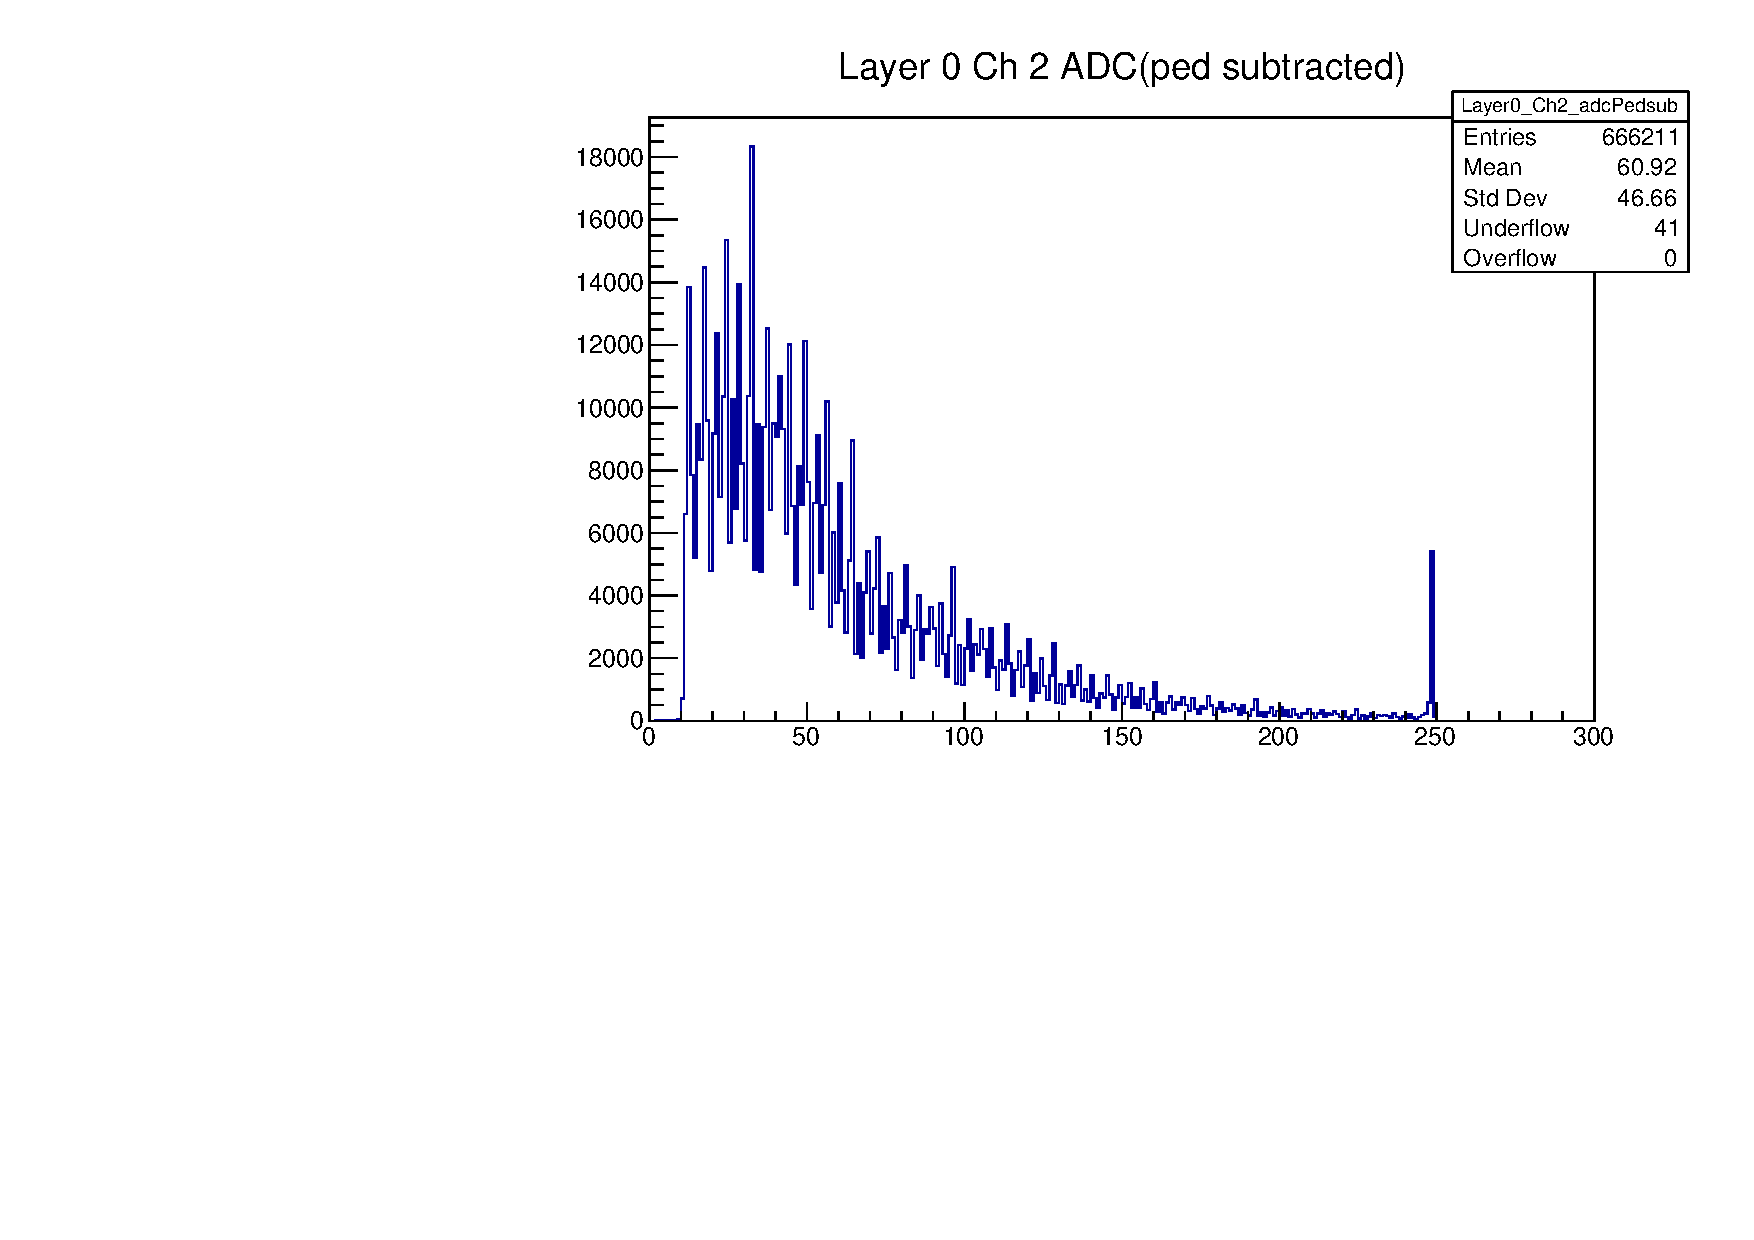
\includegraphics[width=0.33\textwidth,scale=0.5,trim=0 0 0 0,clip]{plotsdir/file0_test-Layer0_Ch2_adcPedsub-1.pdf} 
\caption{(a)Layer 0 Ch 2 ADC[0] ~~~(b) Layer 0 Ch 2 ADC[1] ~~~(c)Layer 0 Ch 2 ADC(ped subtracted) } 
\end{figure} 
\begin{figure}[H] 
\vspace*{-0.3cm} 
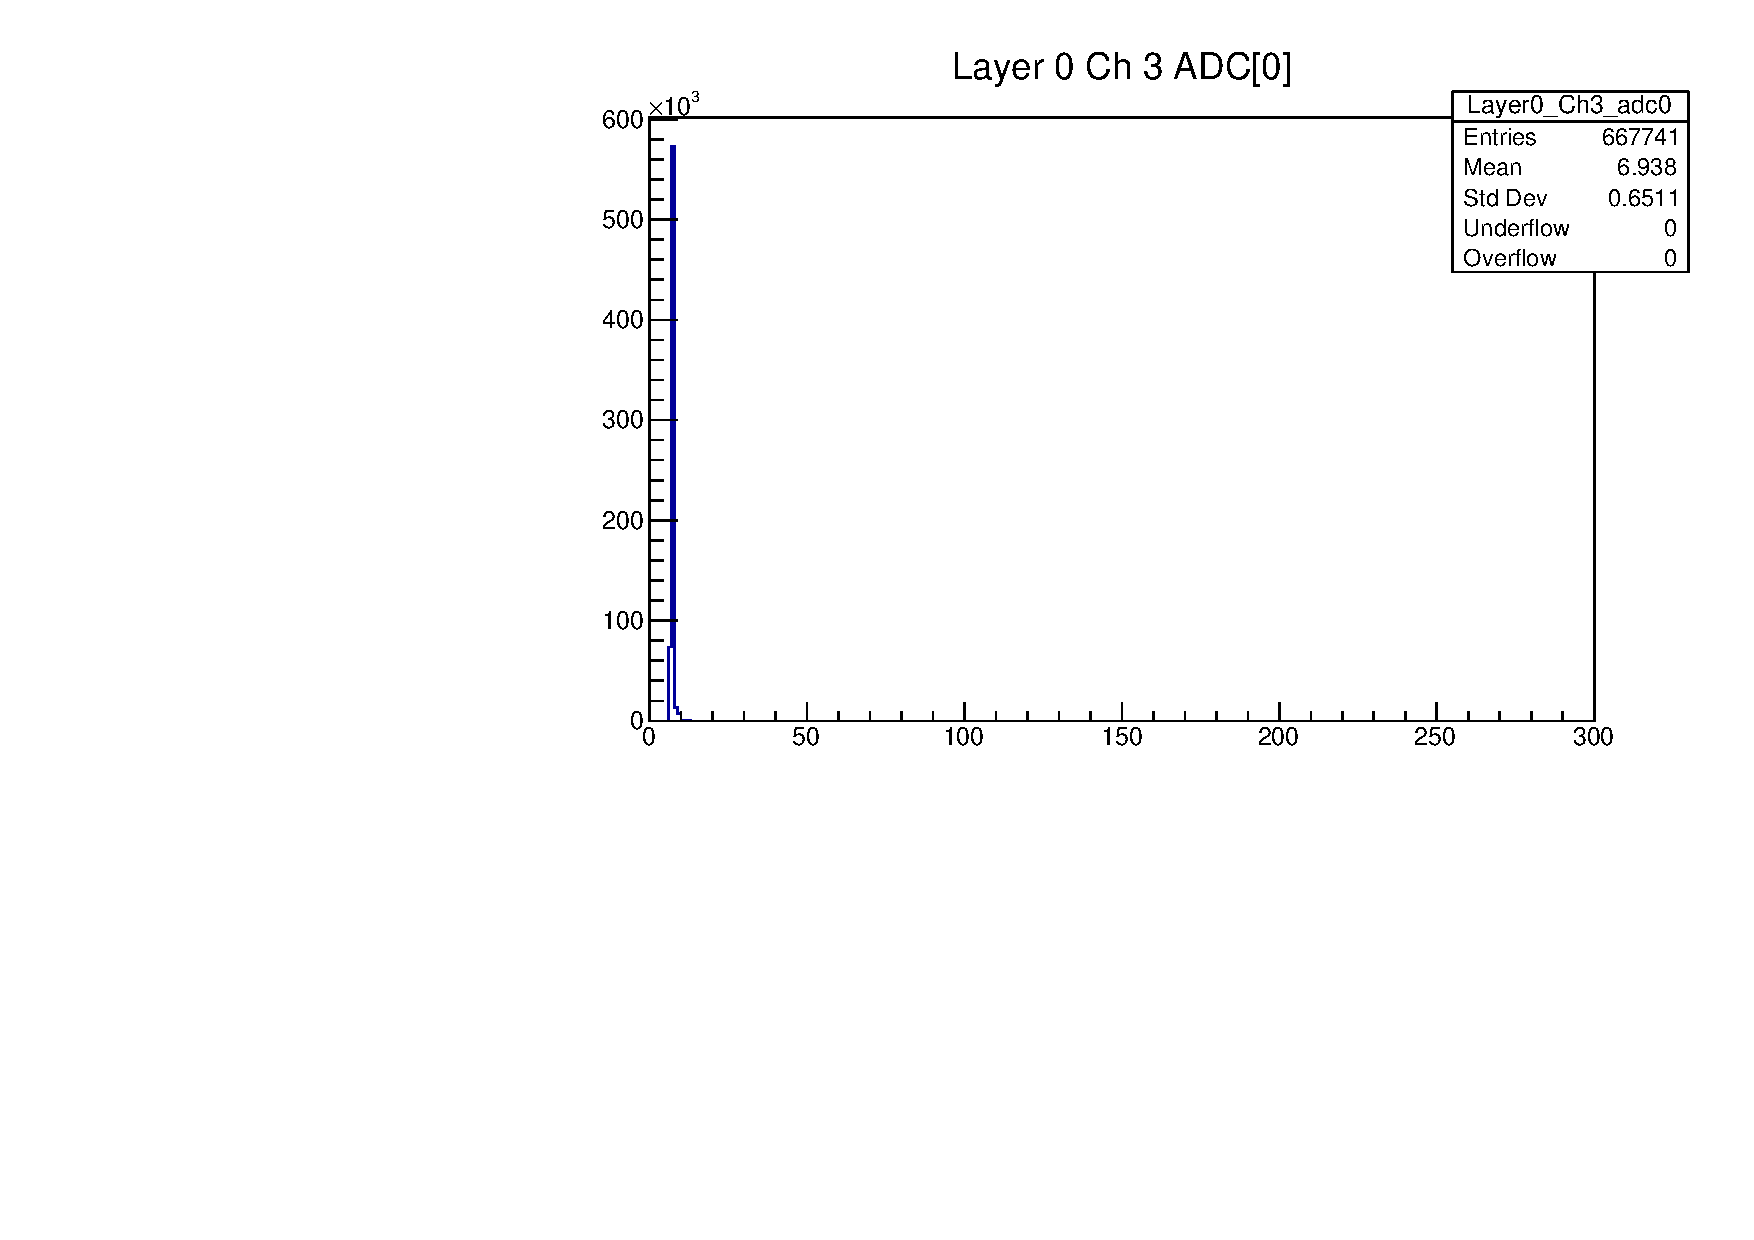
\includegraphics[width=0.33\textwidth,scale=0.5,trim=0 0 0 0,clip]{plotsdir/file0_test-Layer0_Ch3_adc0-1.pdf} 
\includegraphics[width=0.33\textwidth,scale=0.5,trim=0 0 0 0,clip]{plotsdir/file0_test-Layer0_Ch3_adc1-1.pdf} 
\includegraphics[width=0.33\textwidth,scale=0.5,trim=0 0 0 0,clip]{plotsdir/file0_test-Layer0_Ch3_adcPedsub-1.pdf} 
\caption{(a)Layer 0 Ch 3 ADC[0] ~~~(b) Layer 0 Ch 3 ADC[1] ~~~(c)Layer 0 Ch 3 ADC(ped subtracted) } 
\end{figure} 
\begin{figure}[H] 
\vspace*{-0.3cm} 
\includegraphics[width=0.33\textwidth,scale=0.5,trim=0 0 0 0,clip]{plotsdir/file0_test-Layer0_Ch4_adc0-1.pdf} 
\includegraphics[width=0.33\textwidth,scale=0.5,trim=0 0 0 0,clip]{plotsdir/file0_test-Layer0_Ch4_adc1-1.pdf} 
\includegraphics[width=0.33\textwidth,scale=0.5,trim=0 0 0 0,clip]{plotsdir/file0_test-Layer0_Ch4_adcPedsub-1.pdf} 
\caption{(a)Layer 0 Ch 4 ADC[0] ~~~(b) Layer 0 Ch 4 ADC[1] ~~~(c)Layer 0 Ch 4 ADC(ped subtracted) } 
\end{figure} 
\begin{figure}[H] 
\vspace*{-0.3cm} 
\includegraphics[width=0.33\textwidth,scale=0.5,trim=0 0 0 0,clip]{plotsdir/file0_test-Layer0_Ch5_adc0-1.pdf} 
\includegraphics[width=0.33\textwidth,scale=0.5,trim=0 0 0 0,clip]{plotsdir/file0_test-Layer0_Ch5_adc1-1.pdf} 
\includegraphics[width=0.33\textwidth,scale=0.5,trim=0 0 0 0,clip]{plotsdir/file0_test-Layer0_Ch5_adcPedsub-1.pdf} 
\caption{(a)Layer 0 Ch 5 ADC[0] ~~~(b) Layer 0 Ch 5 ADC[1] ~~~(c)Layer 0 Ch 5 ADC(ped subtracted) } 
\end{figure} 
\begin{figure}[H] 
\vspace*{-0.3cm} 
\includegraphics[width=0.33\textwidth,scale=0.5,trim=0 0 0 0,clip]{plotsdir/file0_test-Layer0_Ch6_adc0-1.pdf} 
\includegraphics[width=0.33\textwidth,scale=0.5,trim=0 0 0 0,clip]{plotsdir/file0_test-Layer0_Ch6_adc1-1.pdf} 
\includegraphics[width=0.33\textwidth,scale=0.5,trim=0 0 0 0,clip]{plotsdir/file0_test-Layer0_Ch6_adcPedsub-1.pdf} 
\caption{(a)Layer 0 Ch 6 ADC[0] ~~~(b) Layer 0 Ch 6 ADC[1] ~~~(c)Layer 0 Ch 6 ADC(ped subtracted) } 
\end{figure} 
\begin{figure}[H] 
\vspace*{-0.3cm} 
\includegraphics[width=0.33\textwidth,scale=0.5,trim=0 0 0 0,clip]{plotsdir/file0_test-Layer0_Ch7_adc0-1.pdf} 
\includegraphics[width=0.33\textwidth,scale=0.5,trim=0 0 0 0,clip]{plotsdir/file0_test-Layer0_Ch7_adc1-1.pdf} 
\includegraphics[width=0.33\textwidth,scale=0.5,trim=0 0 0 0,clip]{plotsdir/file0_test-Layer0_Ch7_adcPedsub-1.pdf} 
\caption{(a)Layer 0 Ch 7 ADC[0] ~~~(b) Layer 0 Ch 7 ADC[1] ~~~(c)Layer 0 Ch 7 ADC(ped subtracted) } 
\end{figure} 
\begin{figure}[H] 
\vspace*{-0.3cm} 
\includegraphics[width=0.33\textwidth,scale=0.5,trim=0 0 0 0,clip]{plotsdir/file0_test-Layer0_Ch8_adc0-1.pdf} 
\includegraphics[width=0.33\textwidth,scale=0.5,trim=0 0 0 0,clip]{plotsdir/file0_test-Layer0_Ch8_adc1-1.pdf} 
\includegraphics[width=0.33\textwidth,scale=0.5,trim=0 0 0 0,clip]{plotsdir/file0_test-Layer0_Ch8_adcPedsub-1.pdf} 
\caption{(a)Layer 0 Ch 8 ADC[0] ~~~(b) Layer 0 Ch 8 ADC[1] ~~~(c)Layer 0 Ch 8 ADC(ped subtracted) } 
\end{figure} 
\begin{figure}[H] 
\vspace*{-0.3cm} 
\includegraphics[width=0.33\textwidth,scale=0.5,trim=0 0 0 0,clip]{plotsdir/file0_test-Layer0_Ch9_adc0-1.pdf} 
\includegraphics[width=0.33\textwidth,scale=0.5,trim=0 0 0 0,clip]{plotsdir/file0_test-Layer0_Ch9_adc1-1.pdf} 
\includegraphics[width=0.33\textwidth,scale=0.5,trim=0 0 0 0,clip]{plotsdir/file0_test-Layer0_Ch9_adcPedsub-1.pdf} 
\caption{(a)Layer 0 Ch 9 ADC[0] ~~~(b) Layer 0 Ch 9 ADC[1] ~~~(c)Layer 0 Ch 9 ADC(ped subtracted) } 
\end{figure} 
\begin{figure}[H] 
\vspace*{-0.3cm} 
\includegraphics[width=0.33\textwidth,scale=0.5,trim=0 0 0 0,clip]{plotsdir/file0_test-Layer0_Ch10_adc0-1.pdf} 
\includegraphics[width=0.33\textwidth,scale=0.5,trim=0 0 0 0,clip]{plotsdir/file0_test-Layer0_Ch10_adc1-1.pdf} 
\includegraphics[width=0.33\textwidth,scale=0.5,trim=0 0 0 0,clip]{plotsdir/file0_test-Layer0_Ch10_adcPedsub-1.pdf} 
\caption{(a)Layer 0 Ch 10 ADC[0] ~~~(b) Layer 0 Ch 10 ADC[1] ~~~(c)Layer 0 Ch 10 ADC(ped subtracted) } 
\end{figure} 
\begin{figure}[H] 
\vspace*{-0.3cm} 
\includegraphics[width=0.33\textwidth,scale=0.5,trim=0 0 0 0,clip]{plotsdir/file0_test-Layer1_Ch0_adc0-1.pdf} 
\includegraphics[width=0.33\textwidth,scale=0.5,trim=0 0 0 0,clip]{plotsdir/file0_test-Layer1_Ch0_adc1-1.pdf} 
\includegraphics[width=0.33\textwidth,scale=0.5,trim=0 0 0 0,clip]{plotsdir/file0_test-Layer1_Ch0_adcPedsub-1.pdf} 
\caption{(a)Layer 1 Ch 0 ADC[0] ~~~(b) Layer 1 Ch 0 ADC[1] ~~~(c)Layer 1 Ch 0 ADC(ped subtracted) } 
\end{figure} 
\begin{figure}[H] 
\vspace*{-0.3cm} 
\includegraphics[width=0.33\textwidth,scale=0.5,trim=0 0 0 0,clip]{plotsdir/file0_test-Layer1_Ch1_adc0-1.pdf} 
\includegraphics[width=0.33\textwidth,scale=0.5,trim=0 0 0 0,clip]{plotsdir/file0_test-Layer1_Ch1_adc1-1.pdf} 
\includegraphics[width=0.33\textwidth,scale=0.5,trim=0 0 0 0,clip]{plotsdir/file0_test-Layer1_Ch1_adcPedsub-1.pdf} 
\caption{(a)Layer 1 Ch 1 ADC[0] ~~~(b) Layer 1 Ch 1 ADC[1] ~~~(c)Layer 1 Ch 1 ADC(ped subtracted) } 
\end{figure} 
\begin{figure}[H] 
\vspace*{-0.3cm} 
\includegraphics[width=0.33\textwidth,scale=0.5,trim=0 0 0 0,clip]{plotsdir/file0_test-Layer1_Ch3_adc0-1.pdf} 
\includegraphics[width=0.33\textwidth,scale=0.5,trim=0 0 0 0,clip]{plotsdir/file0_test-Layer1_Ch3_adc1-1.pdf} 
\includegraphics[width=0.33\textwidth,scale=0.5,trim=0 0 0 0,clip]{plotsdir/file0_test-Layer1_Ch3_adcPedsub-1.pdf} 
\caption{(a)Layer 1 Ch 3 ADC[0] ~~~(b) Layer 1 Ch 3 ADC[1] ~~~(c)Layer 1 Ch 3 ADC(ped subtracted) } 
\end{figure} 
\begin{figure}[H] 
\vspace*{-0.3cm} 
\includegraphics[width=0.33\textwidth,scale=0.5,trim=0 0 0 0,clip]{plotsdir/file0_test-Layer1_Ch4_adc0-1.pdf} 
\includegraphics[width=0.33\textwidth,scale=0.5,trim=0 0 0 0,clip]{plotsdir/file0_test-Layer1_Ch4_adc1-1.pdf} 
\includegraphics[width=0.33\textwidth,scale=0.5,trim=0 0 0 0,clip]{plotsdir/file0_test-Layer1_Ch4_adcPedsub-1.pdf} 
\caption{(a)Layer 1 Ch 4 ADC[0] ~~~(b) Layer 1 Ch 4 ADC[1] ~~~(c)Layer 1 Ch 4 ADC(ped subtracted) } 
\end{figure} 
\begin{figure}[H] 
\vspace*{-0.3cm} 
\includegraphics[width=0.33\textwidth,scale=0.5,trim=0 0 0 0,clip]{plotsdir/file0_test-Layer1_Ch5_adc0-1.pdf} 
\includegraphics[width=0.33\textwidth,scale=0.5,trim=0 0 0 0,clip]{plotsdir/file0_test-Layer1_Ch5_adc1-1.pdf} 
\includegraphics[width=0.33\textwidth,scale=0.5,trim=0 0 0 0,clip]{plotsdir/file0_test-Layer1_Ch5_adcPedsub-1.pdf} 
\caption{(a)Layer 1 Ch 5 ADC[0] ~~~(b) Layer 1 Ch 5 ADC[1] ~~~(c)Layer 1 Ch 5 ADC(ped subtracted) } 
\end{figure} 
\begin{figure}[H] 
\vspace*{-0.3cm} 
\includegraphics[width=0.33\textwidth,scale=0.5,trim=0 0 0 0,clip]{plotsdir/file0_test-Layer1_Ch7_adc0-1.pdf} 
\includegraphics[width=0.33\textwidth,scale=0.5,trim=0 0 0 0,clip]{plotsdir/file0_test-Layer1_Ch7_adc1-1.pdf} 
\includegraphics[width=0.33\textwidth,scale=0.5,trim=0 0 0 0,clip]{plotsdir/file0_test-Layer1_Ch7_adcPedsub-1.pdf} 
\caption{(a)Layer 1 Ch 7 ADC[0] ~~~(b) Layer 1 Ch 7 ADC[1] ~~~(c)Layer 1 Ch 7 ADC(ped subtracted) } 
\end{figure} 
\clearpage 
\begin{figure}[H] 
\vspace*{-0.3cm} 
\includegraphics[width=0.33\textwidth,scale=0.5,trim=0 0 0 0,clip]{plotsdir/file0_test-Layer1_Ch8_adc0-1.pdf} 
\includegraphics[width=0.33\textwidth,scale=0.5,trim=0 0 0 0,clip]{plotsdir/file0_test-Layer1_Ch8_adc1-1.pdf} 
\includegraphics[width=0.33\textwidth,scale=0.5,trim=0 0 0 0,clip]{plotsdir/file0_test-Layer1_Ch8_adcPedsub-1.pdf} 
\caption{(a)Layer 1 Ch 8 ADC[0] ~~~(b) Layer 1 Ch 8 ADC[1] ~~~(c)Layer 1 Ch 8 ADC(ped subtracted) } 
\end{figure} 
\begin{figure}[H] 
\vspace*{-0.3cm} 
\includegraphics[width=0.33\textwidth,scale=0.5,trim=0 0 0 0,clip]{plotsdir/file0_test-Layer1_Ch9_adc0-1.pdf} 
\includegraphics[width=0.33\textwidth,scale=0.5,trim=0 0 0 0,clip]{plotsdir/file0_test-Layer1_Ch9_adc1-1.pdf} 
\includegraphics[width=0.33\textwidth,scale=0.5,trim=0 0 0 0,clip]{plotsdir/file0_test-Layer1_Ch9_adcPedsub-1.pdf} 
\caption{(a)Layer 1 Ch 9 ADC[0] ~~~(b) Layer 1 Ch 9 ADC[1] ~~~(c)Layer 1 Ch 9 ADC(ped subtracted) } 
\end{figure} 
\begin{figure}[H] 
\vspace*{-0.3cm} 
\includegraphics[width=0.33\textwidth,scale=0.5,trim=0 0 0 0,clip]{plotsdir/file0_test-Layer2_Ch0_adc0-1.pdf} 
\includegraphics[width=0.33\textwidth,scale=0.5,trim=0 0 0 0,clip]{plotsdir/file0_test-Layer2_Ch0_adc1-1.pdf} 
\includegraphics[width=0.33\textwidth,scale=0.5,trim=0 0 0 0,clip]{plotsdir/file0_test-Layer2_Ch0_adcPedsub-1.pdf} 
\caption{(a)Layer 2 Ch 0 ADC[0] ~~~(b) Layer 2 Ch 0 ADC[1] ~~~(c)Layer 2 Ch 0 ADC(ped subtracted) } 
\end{figure} 
\begin{figure}[H] 
\vspace*{-0.3cm} 
\includegraphics[width=0.33\textwidth,scale=0.5,trim=0 0 0 0,clip]{plotsdir/file0_test-Layer2_Ch1_adc0-1.pdf} 
\includegraphics[width=0.33\textwidth,scale=0.5,trim=0 0 0 0,clip]{plotsdir/file0_test-Layer2_Ch1_adc1-1.pdf} 
\includegraphics[width=0.33\textwidth,scale=0.5,trim=0 0 0 0,clip]{plotsdir/file0_test-Layer2_Ch1_adcPedsub-1.pdf} 
\caption{(a)Layer 2 Ch 1 ADC[0] ~~~(b) Layer 2 Ch 1 ADC[1] ~~~(c)Layer 2 Ch 1 ADC(ped subtracted) } 
\end{figure} 
\begin{figure}[H] 
\vspace*{-0.3cm} 
\includegraphics[width=0.33\textwidth,scale=0.5,trim=0 0 0 0,clip]{plotsdir/file0_test-Layer2_Ch2_adc0-1.pdf} 
\includegraphics[width=0.33\textwidth,scale=0.5,trim=0 0 0 0,clip]{plotsdir/file0_test-Layer2_Ch2_adc1-1.pdf} 
\includegraphics[width=0.33\textwidth,scale=0.5,trim=0 0 0 0,clip]{plotsdir/file0_test-Layer2_Ch2_adcPedsub-1.pdf} 
\caption{(a)Layer 2 Ch 2 ADC[0] ~~~(b) Layer 2 Ch 2 ADC[1] ~~~(c)Layer 2 Ch 2 ADC(ped subtracted) } 
\end{figure} 
\begin{figure}[H] 
\vspace*{-0.3cm} 
\includegraphics[width=0.33\textwidth,scale=0.5,trim=0 0 0 0,clip]{plotsdir/file0_test-Layer2_Ch3_adc0-1.pdf} 
\includegraphics[width=0.33\textwidth,scale=0.5,trim=0 0 0 0,clip]{plotsdir/file0_test-Layer2_Ch3_adc1-1.pdf} 
\includegraphics[width=0.33\textwidth,scale=0.5,trim=0 0 0 0,clip]{plotsdir/file0_test-Layer2_Ch3_adcPedsub-1.pdf} 
\caption{(a)Layer 2 Ch 3 ADC[0] ~~~(b) Layer 2 Ch 3 ADC[1] ~~~(c)Layer 2 Ch 3 ADC(ped subtracted) } 
\end{figure} 
\begin{figure}[H] 
\vspace*{-0.3cm} 
\includegraphics[width=0.33\textwidth,scale=0.5,trim=0 0 0 0,clip]{plotsdir/file0_test-Layer2_Ch4_adc0-1.pdf} 
\includegraphics[width=0.33\textwidth,scale=0.5,trim=0 0 0 0,clip]{plotsdir/file0_test-Layer2_Ch4_adc1-1.pdf} 
\includegraphics[width=0.33\textwidth,scale=0.5,trim=0 0 0 0,clip]{plotsdir/file0_test-Layer2_Ch4_adcPedsub-1.pdf} 
\caption{(a)Layer 2 Ch 4 ADC[0] ~~~(b) Layer 2 Ch 4 ADC[1] ~~~(c)Layer 2 Ch 4 ADC(ped subtracted) } 
\end{figure} 
\begin{figure}[H] 
\vspace*{-0.3cm} 
\includegraphics[width=0.33\textwidth,scale=0.5,trim=0 0 0 0,clip]{plotsdir/file0_test-Layer2_Ch5_adc0-1.pdf} 
\includegraphics[width=0.33\textwidth,scale=0.5,trim=0 0 0 0,clip]{plotsdir/file0_test-Layer2_Ch5_adc1-1.pdf} 
\includegraphics[width=0.33\textwidth,scale=0.5,trim=0 0 0 0,clip]{plotsdir/file0_test-Layer2_Ch5_adcPedsub-1.pdf} 
\caption{(a)Layer 2 Ch 5 ADC[0] ~~~(b) Layer 2 Ch 5 ADC[1] ~~~(c)Layer 2 Ch 5 ADC(ped subtracted) } 
\end{figure} 
\begin{figure}[H] 
\vspace*{-0.3cm} 
\includegraphics[width=0.33\textwidth,scale=0.5,trim=0 0 0 0,clip]{plotsdir/file0_test-Layer2_Ch6_adc0-1.pdf} 
\includegraphics[width=0.33\textwidth,scale=0.5,trim=0 0 0 0,clip]{plotsdir/file0_test-Layer2_Ch6_adc1-1.pdf} 
\includegraphics[width=0.33\textwidth,scale=0.5,trim=0 0 0 0,clip]{plotsdir/file0_test-Layer2_Ch6_adcPedsub-1.pdf} 
\caption{(a)Layer 2 Ch 6 ADC[0] ~~~(b) Layer 2 Ch 6 ADC[1] ~~~(c)Layer 2 Ch 6 ADC(ped subtracted) } 
\end{figure} 
\begin{figure}[H] 
\vspace*{-0.3cm} 
\includegraphics[width=0.33\textwidth,scale=0.5,trim=0 0 0 0,clip]{plotsdir/file0_test-Layer2_Ch7_adc0-1.pdf} 
\includegraphics[width=0.33\textwidth,scale=0.5,trim=0 0 0 0,clip]{plotsdir/file0_test-Layer2_Ch7_adc1-1.pdf} 
\includegraphics[width=0.33\textwidth,scale=0.5,trim=0 0 0 0,clip]{plotsdir/file0_test-Layer2_Ch7_adcPedsub-1.pdf} 
\caption{(a)Layer 2 Ch 7 ADC[0] ~~~(b) Layer 2 Ch 7 ADC[1] ~~~(c)Layer 2 Ch 7 ADC(ped subtracted) } 
\end{figure} 
\begin{figure}[H] 
\vspace*{-0.3cm} 
\includegraphics[width=0.33\textwidth,scale=0.5,trim=0 0 0 0,clip]{plotsdir/file0_test-Layer2_Ch8_adc0-1.pdf} 
\includegraphics[width=0.33\textwidth,scale=0.5,trim=0 0 0 0,clip]{plotsdir/file0_test-Layer2_Ch8_adc1-1.pdf} 
\includegraphics[width=0.33\textwidth,scale=0.5,trim=0 0 0 0,clip]{plotsdir/file0_test-Layer2_Ch8_adcPedsub-1.pdf} 
\caption{(a)Layer 2 Ch 8 ADC[0] ~~~(b) Layer 2 Ch 8 ADC[1] ~~~(c)Layer 2 Ch 8 ADC(ped subtracted) } 
\end{figure} 
\begin{figure}[H] 
\vspace*{-0.3cm} 
\includegraphics[width=0.33\textwidth,scale=0.5,trim=0 0 0 0,clip]{plotsdir/file0_test-Layer2_Ch9_adc0-1.pdf} 
\includegraphics[width=0.33\textwidth,scale=0.5,trim=0 0 0 0,clip]{plotsdir/file0_test-Layer2_Ch9_adc1-1.pdf} 
\includegraphics[width=0.33\textwidth,scale=0.5,trim=0 0 0 0,clip]{plotsdir/file0_test-Layer2_Ch9_adcPedsub-1.pdf} 
\caption{(a)Layer 2 Ch 9 ADC[0] ~~~(b) Layer 2 Ch 9 ADC[1] ~~~(c)Layer 2 Ch 9 ADC(ped subtracted) } 
\end{figure} 
\begin{figure}[H] 
\vspace*{-0.3cm} 
\includegraphics[width=0.33\textwidth,scale=0.5,trim=0 0 0 0,clip]{plotsdir/file0_test-Layer3_Ch0_adc0-1.pdf} 
\includegraphics[width=0.33\textwidth,scale=0.5,trim=0 0 0 0,clip]{plotsdir/file0_test-Layer3_Ch0_adc1-1.pdf} 
\includegraphics[width=0.33\textwidth,scale=0.5,trim=0 0 0 0,clip]{plotsdir/file0_test-Layer3_Ch0_adcPedsub-1.pdf} 
\caption{(a)Layer 3 Ch 0 ADC[0] ~~~(b) Layer 3 Ch 0 ADC[1] ~~~(c)Layer 3 Ch 0 ADC(ped subtracted) } 
\end{figure} 
\begin{figure}[H] 
\vspace*{-0.3cm} 
\includegraphics[width=0.33\textwidth,scale=0.5,trim=0 0 0 0,clip]{plotsdir/file0_test-Layer3_Ch1_adc0-1.pdf} 
\includegraphics[width=0.33\textwidth,scale=0.5,trim=0 0 0 0,clip]{plotsdir/file0_test-Layer3_Ch1_adc1-1.pdf} 
\includegraphics[width=0.33\textwidth,scale=0.5,trim=0 0 0 0,clip]{plotsdir/file0_test-Layer3_Ch1_adcPedsub-1.pdf} 
\caption{(a)Layer 3 Ch 1 ADC[0] ~~~(b) Layer 3 Ch 1 ADC[1] ~~~(c)Layer 3 Ch 1 ADC(ped subtracted) } 
\end{figure} 
\begin{figure}[H] 
\vspace*{-0.3cm} 
\includegraphics[width=0.33\textwidth,scale=0.5,trim=0 0 0 0,clip]{plotsdir/file0_test-Layer3_Ch2_adc0-1.pdf} 
\includegraphics[width=0.33\textwidth,scale=0.5,trim=0 0 0 0,clip]{plotsdir/file0_test-Layer3_Ch2_adc1-1.pdf} 
\includegraphics[width=0.33\textwidth,scale=0.5,trim=0 0 0 0,clip]{plotsdir/file0_test-Layer3_Ch2_adcPedsub-1.pdf} 
\caption{(a)Layer 3 Ch 2 ADC[0] ~~~(b) Layer 3 Ch 2 ADC[1] ~~~(c)Layer 3 Ch 2 ADC(ped subtracted) } 
\end{figure} 
\clearpage 
\begin{figure}[H] 
\vspace*{-0.3cm} 
\includegraphics[width=0.33\textwidth,scale=0.5,trim=0 0 0 0,clip]{plotsdir/file0_test-Layer3_Ch3_adc0-1.pdf} 
\includegraphics[width=0.33\textwidth,scale=0.5,trim=0 0 0 0,clip]{plotsdir/file0_test-Layer3_Ch3_adc1-1.pdf} 
\includegraphics[width=0.33\textwidth,scale=0.5,trim=0 0 0 0,clip]{plotsdir/file0_test-Layer3_Ch3_adcPedsub-1.pdf} 
\caption{(a)Layer 3 Ch 3 ADC[0] ~~~(b) Layer 3 Ch 3 ADC[1] ~~~(c)Layer 3 Ch 3 ADC(ped subtracted) } 
\end{figure} 
\begin{figure}[H] 
\vspace*{-0.3cm} 
\includegraphics[width=0.33\textwidth,scale=0.5,trim=0 0 0 0,clip]{plotsdir/file0_test-Layer3_Ch4_adc0-1.pdf} 
\includegraphics[width=0.33\textwidth,scale=0.5,trim=0 0 0 0,clip]{plotsdir/file0_test-Layer3_Ch4_adc1-1.pdf} 
\includegraphics[width=0.33\textwidth,scale=0.5,trim=0 0 0 0,clip]{plotsdir/file0_test-Layer3_Ch4_adcPedsub-1.pdf} 
\caption{(a)Layer 3 Ch 4 ADC[0] ~~~(b) Layer 3 Ch 4 ADC[1] ~~~(c)Layer 3 Ch 4 ADC(ped subtracted) } 
\end{figure} 
\begin{figure}[H] 
\vspace*{-0.3cm} 
\includegraphics[width=0.33\textwidth,scale=0.5,trim=0 0 0 0,clip]{plotsdir/file0_test-Layer3_Ch5_adc0-1.pdf} 
\includegraphics[width=0.33\textwidth,scale=0.5,trim=0 0 0 0,clip]{plotsdir/file0_test-Layer3_Ch5_adc1-1.pdf} 
\includegraphics[width=0.33\textwidth,scale=0.5,trim=0 0 0 0,clip]{plotsdir/file0_test-Layer3_Ch5_adcPedsub-1.pdf} 
\caption{(a)Layer 3 Ch 5 ADC[0] ~~~(b) Layer 3 Ch 5 ADC[1] ~~~(c)Layer 3 Ch 5 ADC(ped subtracted) } 
\end{figure} 
\begin{figure}[H] 
\vspace*{-0.3cm} 
\includegraphics[width=0.33\textwidth,scale=0.5,trim=0 0 0 0,clip]{plotsdir/file0_test-Layer3_Ch6_adc0-1.pdf} 
\includegraphics[width=0.33\textwidth,scale=0.5,trim=0 0 0 0,clip]{plotsdir/file0_test-Layer3_Ch6_adc1-1.pdf} 
\includegraphics[width=0.33\textwidth,scale=0.5,trim=0 0 0 0,clip]{plotsdir/file0_test-Layer3_Ch6_adcPedsub-1.pdf} 
\caption{(a)Layer 3 Ch 6 ADC[0] ~~~(b) Layer 3 Ch 6 ADC[1] ~~~(c)Layer 3 Ch 6 ADC(ped subtracted) } 
\end{figure} 
\begin{figure}[H] 
\vspace*{-0.3cm} 
\includegraphics[width=0.33\textwidth,scale=0.5,trim=0 0 0 0,clip]{plotsdir/file0_test-Layer3_Ch7_adc0-1.pdf} 
\includegraphics[width=0.33\textwidth,scale=0.5,trim=0 0 0 0,clip]{plotsdir/file0_test-Layer3_Ch7_adc1-1.pdf} 
\includegraphics[width=0.33\textwidth,scale=0.5,trim=0 0 0 0,clip]{plotsdir/file0_test-Layer3_Ch7_adcPedsub-1.pdf} 
\caption{(a)Layer 3 Ch 7 ADC[0] ~~~(b) Layer 3 Ch 7 ADC[1] ~~~(c)Layer 3 Ch 7 ADC(ped subtracted) } 
\end{figure} 
\begin{figure}[H] 
\vspace*{-0.3cm} 
\includegraphics[width=0.33\textwidth,scale=0.5,trim=0 0 0 0,clip]{plotsdir/file0_test-Layer3_Ch8_adc0-1.pdf} 
\includegraphics[width=0.33\textwidth,scale=0.5,trim=0 0 0 0,clip]{plotsdir/file0_test-Layer3_Ch8_adc1-1.pdf} 
\includegraphics[width=0.33\textwidth,scale=0.5,trim=0 0 0 0,clip]{plotsdir/file0_test-Layer3_Ch8_adcPedsub-1.pdf} 
\caption{(a)Layer 3 Ch 8 ADC[0] ~~~(b) Layer 3 Ch 8 ADC[1] ~~~(c)Layer 3 Ch 8 ADC(ped subtracted) } 
\end{figure} 
\begin{figure}[H] 
\vspace*{-0.3cm} 
\includegraphics[width=0.33\textwidth,scale=0.5,trim=0 0 0 0,clip]{plotsdir/file0_test-Layer3_Ch9_adc0-1.pdf} 
\includegraphics[width=0.33\textwidth,scale=0.5,trim=0 0 0 0,clip]{plotsdir/file0_test-Layer3_Ch9_adc1-1.pdf} 
\includegraphics[width=0.33\textwidth,scale=0.5,trim=0 0 0 0,clip]{plotsdir/file0_test-Layer3_Ch9_adcPedsub-1.pdf} 
\caption{(a)Layer 3 Ch 9 ADC[0] ~~~(b) Layer 3 Ch 9 ADC[1] ~~~(c)Layer 3 Ch 9 ADC(ped subtracted) } 
\end{figure} 
\begin{figure}[H] 
\vspace*{-0.3cm} 
\includegraphics[width=0.33\textwidth,scale=0.5,trim=0 0 0 0,clip]{plotsdir/file0_test-dt-1.pdf} 
\includegraphics[width=0.33\textwidth,scale=0.5,trim=0 0 0 0,clip]{plotsdir/file0_test-dt2-1.pdf} 
\includegraphics[width=0.33\textwidth,scale=0.5,trim=0 0 0 0,clip]{plotsdir/file0_test-X0a-1.pdf} 
\caption{(a)hitB-hitA ~~~(b) hitB-hitA ~~~(c)X (layer 0) x-coincidence } 
\end{figure} 
\begin{figure}[H] 
\vspace*{-0.3cm} 
\includegraphics[width=0.33\textwidth,scale=0.5,trim=0 0 0 0,clip]{plotsdir/file0_test-Y1a-1.pdf} 
\includegraphics[width=0.33\textwidth,scale=0.5,trim=0 0 0 0,clip]{plotsdir/file0_test-X0b-1.pdf} 
\includegraphics[width=0.33\textwidth,scale=0.5,trim=0 0 0 0,clip]{plotsdir/file0_test-Y1b-1.pdf} 
\caption{(a)Y (layer 1) y-coincidence ~~~(b) X (layer 0) xy-coincidence ~~~(c)Y (layer 1) xy-coincidence } 
\end{figure} 
\begin{figure}[H] 
\vspace*{-0.3cm} 
\includegraphics[width=0.33\textwidth,scale=0.5,trim=0 0 0 0,clip]{plotsdir/file0_test-nMuonEvents-1.pdf} 
\includegraphics[width=0.33\textwidth,scale=0.5,trim=0 0 0 0,clip]{plotsdir/file0_test-nMuons-1.pdf} 
\includegraphics[width=0.33\textwidth,scale=0.5,trim=0 0 0 0,clip]{plotsdir/file0_test-muX-1.pdf} 
\caption{(a)number of muonEvents ~~~(b) number of muons ~~~(c)muon: X at Z=0 } 
\end{figure} 
\begin{figure}[H] 
\vspace*{-0.3cm} 
\includegraphics[width=0.33\textwidth,scale=0.5,trim=0 0 0 0,clip]{plotsdir/file0_test-muY-1.pdf} 
\includegraphics[width=0.33\textwidth,scale=0.5,trim=0 0 0 0,clip]{plotsdir/file0_test-muXS-1.pdf} 
\includegraphics[width=0.33\textwidth,scale=0.5,trim=0 0 0 0,clip]{plotsdir/file0_test-muYS-1.pdf} 
\caption{(a)muon: Y at Z=0 ~~~(b) muon: X slope (theta x-proj) (deg) ~~~(c)muon: Y slope (theta y-proj) (deg) } 
\end{figure} 
\begin{figure}[H] 
\vspace*{-0.3cm} 
\includegraphics[width=0.33\textwidth,scale=0.5,trim=0 0 0 0,clip]{plotsdir/file0_test-muTheta-1.pdf} 
\caption{(a)muon: theta (deg) } 
\end{figure} 
\newpage 
\section{Hit Cluster Analysis} 
\begin{verbatim} 
Clusters of hits in global time frame. 
\end{verbatim} 
\begin{figure}[H] 
\vspace*{-0.3cm} 
\includegraphics[width=0.33\textwidth,scale=0.5,trim=0 0 0 0,clip]{plotsdir/file0_clusters-nClusters-1.pdf} 
\includegraphics[width=0.33\textwidth,scale=0.5,trim=0 0 0 0,clip]{plotsdir/file0_clusters-nHitsPerCluster-1.pdf} 
\includegraphics[width=0.33\textwidth,scale=0.5,trim=0 0 0 0,clip]{plotsdir/file0_clusters-hcL0Chs-1.pdf} 
\caption{(a)N of Clusters ~~~(b) N of hits per cluster ~~~(c)hit cluster, ch in Layer 0 } 
\end{figure} 
\begin{figure}[H] 
\vspace*{-0.3cm} 
\includegraphics[width=0.33\textwidth,scale=0.5,trim=0 0 0 0,clip]{plotsdir/file0_clusters-hcL1Chs-1.pdf} 
\includegraphics[width=0.33\textwidth,scale=0.5,trim=0 0 0 0,clip]{plotsdir/file0_clusters-hcL2Chs-1.pdf} 
\includegraphics[width=0.33\textwidth,scale=0.5,trim=0 0 0 0,clip]{plotsdir/file0_clusters-hcL3Chs-1.pdf} 
\caption{(a)hit cluster, ch in Layer 1 ~~~(b) hit cluster, ch in Layer 2 ~~~(c)hit cluster, ch in Layer 3 } 
\end{figure} 
\begin{figure}[H] 
\vspace*{-0.3cm} 
\includegraphics[width=0.33\textwidth,scale=0.5,trim=0 0 0 0,clip]{plotsdir/file0_clusters-hcL0nHits-1.pdf} 
\includegraphics[width=0.33\textwidth,scale=0.5,trim=0 0 0 0,clip]{plotsdir/file0_clusters-hcL1nHits-1.pdf} 
\includegraphics[width=0.33\textwidth,scale=0.5,trim=0 0 0 0,clip]{plotsdir/file0_clusters-hcL2nHits-1.pdf} 
\caption{(a)N hits in cluster, Layer 0 ~~~(b) N hits in cluster, Layer 0 ~~~(c)N hits in cluster, Layer 0 } 
\end{figure} 
\begin{figure}[H] 
\vspace*{-0.3cm} 
\includegraphics[width=0.33\textwidth,scale=0.5,trim=0 0 0 0,clip]{plotsdir/file0_clusters-hcL3nHits-1.pdf} 
\caption{(a)N hits in cluster, Layer 0 } 
\end{figure} 
\newpage 
\section{Muon Track Analysis} 
\begin{verbatim} 
Four layer coincidence. 
The number of hits on muon track = 1 hit per layer  
\end{verbatim} 
\begin{figure}[H] 
\vspace*{-0.3cm} 
\includegraphics[width=0.33\textwidth,scale=0.5,trim=0 0 0 0,clip]{plotsdir/file0_muons-nMuonEvents-1.pdf} 
\includegraphics[width=0.33\textwidth,scale=0.5,trim=0 0 0 0,clip]{plotsdir/file0_muons-nMuons-1.pdf} 
\includegraphics[width=0.33\textwidth,scale=0.5,trim=0 0 0 0,clip]{plotsdir/file0_muons-muX-1.pdf} 
\caption{(a)number of muonEvents ~~~(b) number of muons ~~~(c)muon: X at Z=0 } 
\end{figure} 
\begin{figure}[H] 
\vspace*{-0.3cm} 
\includegraphics[width=0.33\textwidth,scale=0.5,trim=0 0 0 0,clip]{plotsdir/file0_muons-muY-1.pdf} 
\includegraphics[width=0.33\textwidth,scale=0.5,trim=0 0 0 0,clip]{plotsdir/file0_muons-muXS-1.pdf} 
\includegraphics[width=0.33\textwidth,scale=0.5,trim=0 0 0 0,clip]{plotsdir/file0_muons-muYS-1.pdf} 
\caption{(a)muon: Y at Z=0 ~~~(b) muon: X slope (theta x-proj) (deg) ~~~(c)muon: Y slope (theta y-proj) (deg) } 
\end{figure} 
\begin{figure}[H] 
\vspace*{-0.3cm} 
\includegraphics[width=0.33\textwidth,scale=0.5,trim=0 0 0 0,clip]{plotsdir/file0_muons-muTheta-1.pdf} 
\includegraphics[width=0.33\textwidth,scale=0.5,trim=0 0 0 0,clip]{plotsdir/file0_muons-N1MasterTime-1.pdf} 
\includegraphics[width=0.33\textwidth,scale=0.5,trim=0 0 0 0,clip]{plotsdir/file0_muons-N2MasterTime-1.pdf} 
\caption{(a)muon: theta (deg) ~~~(b) Node 1- Master Time ~~~(c)Node 2- Master Time } 
\end{figure} 
\begin{figure}[H] 
\vspace*{-0.3cm} 
\includegraphics[width=0.33\textwidth,scale=0.5,trim=0 0 0 0,clip]{plotsdir/file0_muons-N3MasterTime-1.pdf} 
\includegraphics[width=0.33\textwidth,scale=0.5,trim=0 0 0 0,clip]{plotsdir/file0_muons-N4MasterTime-1.pdf} 
\includegraphics[width=0.33\textwidth,scale=0.5,trim=0 0 0 0,clip]{plotsdir/file0_muons-N5MasterTime-1.pdf} 
\caption{(a)Node 3- Master Time ~~~(b) Node 4- Master Time ~~~(c)Node 5- Master Time } 
\end{figure} 
\begin{figure}[H] 
\vspace*{-0.3cm} 
\includegraphics[width=0.33\textwidth,scale=0.5,trim=0 0 0 0,clip]{plotsdir/file0_muons-N6MasterTime-1.pdf} 
\includegraphics[width=0.33\textwidth,scale=0.5,trim=0 0 0 0,clip]{plotsdir/file0_muons-N7MasterTime-1.pdf} 
\includegraphics[width=0.33\textwidth,scale=0.5,trim=0 0 0 0,clip]{plotsdir/file0_muons-N8MasterTime-1.pdf} 
\caption{(a)Node 6- Master Time ~~~(b) Node 7- Master Time ~~~(c)Node 8- Master Time } 
\end{figure} 
\begin{figure}[H] 
\vspace*{-0.3cm} 
\includegraphics[width=0.33\textwidth,scale=0.5,trim=0 0 0 0,clip]{plotsdir/file0_muons-nHits-1.pdf} 
\includegraphics[width=0.33\textwidth,scale=0.5,trim=0 0 0 0,clip]{plotsdir/file0_muons-LayerNum-1.pdf} 
\includegraphics[width=0.33\textwidth,scale=0.5,trim=0 0 0 0,clip]{plotsdir/file0_muons-L0Ch-1.pdf} 
\caption{(a)number of hits ~~~(b) Layer Number ~~~(c)L0 Channel Numbers } 
\end{figure} 
\begin{figure}[H] 
\vspace*{-0.3cm} 
\includegraphics[width=0.33\textwidth,scale=0.5,trim=0 0 0 0,clip]{plotsdir/file0_muons-L1Ch-1.pdf} 
\includegraphics[width=0.33\textwidth,scale=0.5,trim=0 0 0 0,clip]{plotsdir/file0_muons-L2Ch-1.pdf} 
\includegraphics[width=0.33\textwidth,scale=0.5,trim=0 0 0 0,clip]{plotsdir/file0_muons-L3Ch-1.pdf} 
\caption{(a)L1 Channel Numbers ~~~(b) L2 Channel Numbers ~~~(c)L3 Channel Numbers } 
\end{figure} 
\begin{figure}[H] 
\vspace*{-0.3cm} 
\includegraphics[width=0.33\textwidth,scale=0.5,trim=0 0 0 0,clip]{plotsdir/file0_muons-adcL0ChAll-1.pdf} 
\includegraphics[width=0.33\textwidth,scale=0.5,trim=0 0 0 0,clip]{plotsdir/file0_muons-adcL1ChAll-1.pdf} 
\includegraphics[width=0.33\textwidth,scale=0.5,trim=0 0 0 0,clip]{plotsdir/file0_muons-adcL2ChAll-1.pdf} 
\caption{(a)L0 ADC ped sub(all channels) ~~~(b) L1 ADC ped sub(all channels) ~~~(c)L2 ADC ped sub (all channels) } 
\end{figure} 
\begin{figure}[H] 
\vspace*{-0.3cm} 
\includegraphics[width=0.33\textwidth,scale=0.5,trim=0 0 0 0,clip]{plotsdir/file0_muons-adcL3ChAll-1.pdf} 
\includegraphics[width=0.33\textwidth,scale=0.5,trim=0 0 0 0,clip]{plotsdir/file0_muons-adcL3ChAll-1.pdf} 
\includegraphics[width=0.33\textwidth,scale=0.5,trim=0 0 0 0,clip]{plotsdir/file0_muons-Layer0_Ch0_adc0-1.pdf} 
\caption{(a)L3 ADC ped sub (all channels) ~~~(b) L3 ADC ped sub (all channels) ~~~(c)Layer 0 Ch 0 ADC[0] } 
\end{figure} 
\begin{figure}[H] 
\vspace*{-0.3cm} 
\includegraphics[width=0.33\textwidth,scale=0.5,trim=0 0 0 0,clip]{plotsdir/file0_muons-Layer0_Ch0_adc0-1.pdf} 
\includegraphics[width=0.33\textwidth,scale=0.5,trim=0 0 0 0,clip]{plotsdir/file0_muons-Layer0_Ch0_adc1-1.pdf} 
\includegraphics[width=0.33\textwidth,scale=0.5,trim=0 0 0 0,clip]{plotsdir/file0_muons-Layer0_Ch0_adcPedsub-1.pdf} 
\caption{(a)Layer 0 Ch 0 ADC[0] ~~~(b) Layer 0 Ch 0 ADC[1] ~~~(c)Layer 0 Ch 0 ADC(ped subtracted) } 
\end{figure} 
\begin{figure}[H] 
\vspace*{-0.3cm} 
\includegraphics[width=0.33\textwidth,scale=0.5,trim=0 0 0 0,clip]{plotsdir/file0_muons-Layer0_Ch1_adc0-1.pdf} 
\includegraphics[width=0.33\textwidth,scale=0.5,trim=0 0 0 0,clip]{plotsdir/file0_muons-Layer0_Ch1_adc1-1.pdf} 
\includegraphics[width=0.33\textwidth,scale=0.5,trim=0 0 0 0,clip]{plotsdir/file0_muons-Layer0_Ch1_adcPedsub-1.pdf} 
\caption{(a)Layer 0 Ch 1 ADC[0] ~~~(b) Layer 0 Ch 1 ADC[1] ~~~(c)Layer 0 Ch 1 ADC(ped subtracted) } 
\end{figure} 
\begin{figure}[H] 
\vspace*{-0.3cm} 
\includegraphics[width=0.33\textwidth,scale=0.5,trim=0 0 0 0,clip]{plotsdir/file0_muons-Layer0_Ch2_adc0-1.pdf} 
\includegraphics[width=0.33\textwidth,scale=0.5,trim=0 0 0 0,clip]{plotsdir/file0_muons-Layer0_Ch2_adc1-1.pdf} 
\includegraphics[width=0.33\textwidth,scale=0.5,trim=0 0 0 0,clip]{plotsdir/file0_muons-Layer0_Ch2_adcPedsub-1.pdf} 
\caption{(a)Layer 0 Ch 2 ADC[0] ~~~(b) Layer 0 Ch 2 ADC[1] ~~~(c)Layer 0 Ch 2 ADC(ped subtracted) } 
\end{figure} 
\begin{figure}[H] 
\vspace*{-0.3cm} 
\includegraphics[width=0.33\textwidth,scale=0.5,trim=0 0 0 0,clip]{plotsdir/file0_muons-Layer0_Ch3_adc0-1.pdf} 
\includegraphics[width=0.33\textwidth,scale=0.5,trim=0 0 0 0,clip]{plotsdir/file0_muons-Layer0_Ch3_adc1-1.pdf} 
\includegraphics[width=0.33\textwidth,scale=0.5,trim=0 0 0 0,clip]{plotsdir/file0_muons-Layer0_Ch3_adcPedsub-1.pdf} 
\caption{(a)Layer 0 Ch 3 ADC[0] ~~~(b) Layer 0 Ch 3 ADC[1] ~~~(c)Layer 0 Ch 3 ADC(ped subtracted) } 
\end{figure} 
\begin{figure}[H] 
\vspace*{-0.3cm} 
\includegraphics[width=0.33\textwidth,scale=0.5,trim=0 0 0 0,clip]{plotsdir/file0_muons-Layer0_Ch4_adc0-1.pdf} 
\includegraphics[width=0.33\textwidth,scale=0.5,trim=0 0 0 0,clip]{plotsdir/file0_muons-Layer0_Ch4_adc1-1.pdf} 
\includegraphics[width=0.33\textwidth,scale=0.5,trim=0 0 0 0,clip]{plotsdir/file0_muons-Layer0_Ch4_adcPedsub-1.pdf} 
\caption{(a)Layer 0 Ch 4 ADC[0] ~~~(b) Layer 0 Ch 4 ADC[1] ~~~(c)Layer 0 Ch 4 ADC(ped subtracted) } 
\end{figure} 
\begin{figure}[H] 
\vspace*{-0.3cm} 
\includegraphics[width=0.33\textwidth,scale=0.5,trim=0 0 0 0,clip]{plotsdir/file0_muons-Layer0_Ch5_adc0-1.pdf} 
\includegraphics[width=0.33\textwidth,scale=0.5,trim=0 0 0 0,clip]{plotsdir/file0_muons-Layer0_Ch5_adc1-1.pdf} 
\includegraphics[width=0.33\textwidth,scale=0.5,trim=0 0 0 0,clip]{plotsdir/file0_muons-Layer0_Ch5_adcPedsub-1.pdf} 
\caption{(a)Layer 0 Ch 5 ADC[0] ~~~(b) Layer 0 Ch 5 ADC[1] ~~~(c)Layer 0 Ch 5 ADC(ped subtracted) } 
\end{figure} 
\clearpage 
\begin{figure}[H] 
\vspace*{-0.3cm} 
\includegraphics[width=0.33\textwidth,scale=0.5,trim=0 0 0 0,clip]{plotsdir/file0_muons-Layer0_Ch6_adc0-1.pdf} 
\includegraphics[width=0.33\textwidth,scale=0.5,trim=0 0 0 0,clip]{plotsdir/file0_muons-Layer0_Ch6_adc1-1.pdf} 
\includegraphics[width=0.33\textwidth,scale=0.5,trim=0 0 0 0,clip]{plotsdir/file0_muons-Layer0_Ch6_adcPedsub-1.pdf} 
\caption{(a)Layer 0 Ch 6 ADC[0] ~~~(b) Layer 0 Ch 6 ADC[1] ~~~(c)Layer 0 Ch 6 ADC(ped subtracted) } 
\end{figure} 
\begin{figure}[H] 
\vspace*{-0.3cm} 
\includegraphics[width=0.33\textwidth,scale=0.5,trim=0 0 0 0,clip]{plotsdir/file0_muons-Layer0_Ch7_adc0-1.pdf} 
\includegraphics[width=0.33\textwidth,scale=0.5,trim=0 0 0 0,clip]{plotsdir/file0_muons-Layer0_Ch7_adc1-1.pdf} 
\includegraphics[width=0.33\textwidth,scale=0.5,trim=0 0 0 0,clip]{plotsdir/file0_muons-Layer0_Ch7_adcPedsub-1.pdf} 
\caption{(a)Layer 0 Ch 7 ADC[0] ~~~(b) Layer 0 Ch 7 ADC[1] ~~~(c)Layer 0 Ch 7 ADC(ped subtracted) } 
\end{figure} 
\begin{figure}[H] 
\vspace*{-0.3cm} 
\includegraphics[width=0.33\textwidth,scale=0.5,trim=0 0 0 0,clip]{plotsdir/file0_muons-Layer0_Ch8_adc0-1.pdf} 
\includegraphics[width=0.33\textwidth,scale=0.5,trim=0 0 0 0,clip]{plotsdir/file0_muons-Layer0_Ch8_adc1-1.pdf} 
\includegraphics[width=0.33\textwidth,scale=0.5,trim=0 0 0 0,clip]{plotsdir/file0_muons-Layer0_Ch8_adcPedsub-1.pdf} 
\caption{(a)Layer 0 Ch 8 ADC[0] ~~~(b) Layer 0 Ch 8 ADC[1] ~~~(c)Layer 0 Ch 8 ADC(ped subtracted) } 
\end{figure} 
\begin{figure}[H] 
\vspace*{-0.3cm} 
\includegraphics[width=0.33\textwidth,scale=0.5,trim=0 0 0 0,clip]{plotsdir/file0_muons-Layer0_Ch9_adc0-1.pdf} 
\includegraphics[width=0.33\textwidth,scale=0.5,trim=0 0 0 0,clip]{plotsdir/file0_muons-Layer0_Ch9_adc1-1.pdf} 
\includegraphics[width=0.33\textwidth,scale=0.5,trim=0 0 0 0,clip]{plotsdir/file0_muons-Layer0_Ch9_adcPedsub-1.pdf} 
\caption{(a)Layer 0 Ch 9 ADC[0] ~~~(b) Layer 0 Ch 9 ADC[1] ~~~(c)Layer 0 Ch 9 ADC(ped subtracted) } 
\end{figure} 
\begin{figure}[H] 
\vspace*{-0.3cm} 
\includegraphics[width=0.33\textwidth,scale=0.5,trim=0 0 0 0,clip]{plotsdir/file0_muons-Layer0_Ch10_adc0-1.pdf} 
\includegraphics[width=0.33\textwidth,scale=0.5,trim=0 0 0 0,clip]{plotsdir/file0_muons-Layer0_Ch10_adc1-1.pdf} 
\includegraphics[width=0.33\textwidth,scale=0.5,trim=0 0 0 0,clip]{plotsdir/file0_muons-Layer0_Ch10_adcPedsub-1.pdf} 
\caption{(a)Layer 0 Ch 10 ADC[0] ~~~(b) Layer 0 Ch 10 ADC[1] ~~~(c)Layer 0 Ch 10 ADC(ped subtracted) } 
\end{figure} 
\begin{figure}[H] 
\vspace*{-0.3cm} 
\includegraphics[width=0.33\textwidth,scale=0.5,trim=0 0 0 0,clip]{plotsdir/file0_muons-Layer1_Ch0_adc0-1.pdf} 
\includegraphics[width=0.33\textwidth,scale=0.5,trim=0 0 0 0,clip]{plotsdir/file0_muons-Layer1_Ch0_adc1-1.pdf} 
\includegraphics[width=0.33\textwidth,scale=0.5,trim=0 0 0 0,clip]{plotsdir/file0_muons-Layer1_Ch0_adcPedsub-1.pdf} 
\caption{(a)Layer 1 Ch 0 ADC[0] ~~~(b) Layer 1 Ch 0 ADC[1] ~~~(c)Layer 1 Ch 0 ADC(ped subtracted) } 
\end{figure} 
\begin{figure}[H] 
\vspace*{-0.3cm} 
\includegraphics[width=0.33\textwidth,scale=0.5,trim=0 0 0 0,clip]{plotsdir/file0_muons-Layer1_Ch1_adc0-1.pdf} 
\includegraphics[width=0.33\textwidth,scale=0.5,trim=0 0 0 0,clip]{plotsdir/file0_muons-Layer1_Ch1_adc1-1.pdf} 
\includegraphics[width=0.33\textwidth,scale=0.5,trim=0 0 0 0,clip]{plotsdir/file0_muons-Layer1_Ch1_adcPedsub-1.pdf} 
\caption{(a)Layer 1 Ch 1 ADC[0] ~~~(b) Layer 1 Ch 1 ADC[1] ~~~(c)Layer 1 Ch 1 ADC(ped subtracted) } 
\end{figure} 
\begin{figure}[H] 
\vspace*{-0.3cm} 
\includegraphics[width=0.33\textwidth,scale=0.5,trim=0 0 0 0,clip]{plotsdir/file0_muons-Layer1_Ch3_adc0-1.pdf} 
\includegraphics[width=0.33\textwidth,scale=0.5,trim=0 0 0 0,clip]{plotsdir/file0_muons-Layer1_Ch3_adc1-1.pdf} 
\includegraphics[width=0.33\textwidth,scale=0.5,trim=0 0 0 0,clip]{plotsdir/file0_muons-Layer1_Ch3_adcPedsub-1.pdf} 
\caption{(a)Layer 1 Ch 3 ADC[0] ~~~(b) Layer 1 Ch 3 ADC[1] ~~~(c)Layer 1 Ch 3 ADC(ped subtracted) } 
\end{figure} 
\begin{figure}[H] 
\vspace*{-0.3cm} 
\includegraphics[width=0.33\textwidth,scale=0.5,trim=0 0 0 0,clip]{plotsdir/file0_muons-Layer1_Ch4_adc0-1.pdf} 
\includegraphics[width=0.33\textwidth,scale=0.5,trim=0 0 0 0,clip]{plotsdir/file0_muons-Layer1_Ch4_adc1-1.pdf} 
\includegraphics[width=0.33\textwidth,scale=0.5,trim=0 0 0 0,clip]{plotsdir/file0_muons-Layer1_Ch4_adcPedsub-1.pdf} 
\caption{(a)Layer 1 Ch 4 ADC[0] ~~~(b) Layer 1 Ch 4 ADC[1] ~~~(c)Layer 1 Ch 4 ADC(ped subtracted) } 
\end{figure} 
\begin{figure}[H] 
\vspace*{-0.3cm} 
\includegraphics[width=0.33\textwidth,scale=0.5,trim=0 0 0 0,clip]{plotsdir/file0_muons-Layer1_Ch5_adc0-1.pdf} 
\includegraphics[width=0.33\textwidth,scale=0.5,trim=0 0 0 0,clip]{plotsdir/file0_muons-Layer1_Ch5_adc1-1.pdf} 
\includegraphics[width=0.33\textwidth,scale=0.5,trim=0 0 0 0,clip]{plotsdir/file0_muons-Layer1_Ch5_adcPedsub-1.pdf} 
\caption{(a)Layer 1 Ch 5 ADC[0] ~~~(b) Layer 1 Ch 5 ADC[1] ~~~(c)Layer 1 Ch 5 ADC(ped subtracted) } 
\end{figure} 
\begin{figure}[H] 
\vspace*{-0.3cm} 
\includegraphics[width=0.33\textwidth,scale=0.5,trim=0 0 0 0,clip]{plotsdir/file0_muons-Layer1_Ch7_adc0-1.pdf} 
\includegraphics[width=0.33\textwidth,scale=0.5,trim=0 0 0 0,clip]{plotsdir/file0_muons-Layer1_Ch7_adc1-1.pdf} 
\includegraphics[width=0.33\textwidth,scale=0.5,trim=0 0 0 0,clip]{plotsdir/file0_muons-Layer1_Ch7_adcPedsub-1.pdf} 
\caption{(a)Layer 1 Ch 7 ADC[0] ~~~(b) Layer 1 Ch 7 ADC[1] ~~~(c)Layer 1 Ch 7 ADC(ped subtracted) } 
\end{figure} 
\begin{figure}[H] 
\vspace*{-0.3cm} 
\includegraphics[width=0.33\textwidth,scale=0.5,trim=0 0 0 0,clip]{plotsdir/file0_muons-Layer1_Ch8_adc0-1.pdf} 
\includegraphics[width=0.33\textwidth,scale=0.5,trim=0 0 0 0,clip]{plotsdir/file0_muons-Layer1_Ch8_adc1-1.pdf} 
\includegraphics[width=0.33\textwidth,scale=0.5,trim=0 0 0 0,clip]{plotsdir/file0_muons-Layer1_Ch8_adcPedsub-1.pdf} 
\caption{(a)Layer 1 Ch 8 ADC[0] ~~~(b) Layer 1 Ch 8 ADC[1] ~~~(c)Layer 1 Ch 8 ADC(ped subtracted) } 
\end{figure} 
\begin{figure}[H] 
\vspace*{-0.3cm} 
\includegraphics[width=0.33\textwidth,scale=0.5,trim=0 0 0 0,clip]{plotsdir/file0_muons-Layer2_Ch0_adc0-1.pdf} 
\includegraphics[width=0.33\textwidth,scale=0.5,trim=0 0 0 0,clip]{plotsdir/file0_muons-Layer2_Ch0_adc1-1.pdf} 
\includegraphics[width=0.33\textwidth,scale=0.5,trim=0 0 0 0,clip]{plotsdir/file0_muons-Layer2_Ch0_adcPedsub-1.pdf} 
\caption{(a)Layer 2 Ch 0 ADC[0] ~~~(b) Layer 2 Ch 0 ADC[1] ~~~(c)Layer 2 Ch 0 ADC(ped subtracted) } 
\end{figure} 
\begin{figure}[H] 
\vspace*{-0.3cm} 
\includegraphics[width=0.33\textwidth,scale=0.5,trim=0 0 0 0,clip]{plotsdir/file0_muons-Layer2_Ch1_adc0-1.pdf} 
\includegraphics[width=0.33\textwidth,scale=0.5,trim=0 0 0 0,clip]{plotsdir/file0_muons-Layer2_Ch1_adc1-1.pdf} 
\includegraphics[width=0.33\textwidth,scale=0.5,trim=0 0 0 0,clip]{plotsdir/file0_muons-Layer2_Ch1_adcPedsub-1.pdf} 
\caption{(a)Layer 2 Ch 1 ADC[0] ~~~(b) Layer 2 Ch 1 ADC[1] ~~~(c)Layer 2 Ch 1 ADC(ped subtracted) } 
\end{figure} 
\begin{figure}[H] 
\vspace*{-0.3cm} 
\includegraphics[width=0.33\textwidth,scale=0.5,trim=0 0 0 0,clip]{plotsdir/file0_muons-Layer2_Ch2_adc0-1.pdf} 
\includegraphics[width=0.33\textwidth,scale=0.5,trim=0 0 0 0,clip]{plotsdir/file0_muons-Layer2_Ch2_adc1-1.pdf} 
\includegraphics[width=0.33\textwidth,scale=0.5,trim=0 0 0 0,clip]{plotsdir/file0_muons-Layer2_Ch2_adcPedsub-1.pdf} 
\caption{(a)Layer 2 Ch 2 ADC[0] ~~~(b) Layer 2 Ch 2 ADC[1] ~~~(c)Layer 2 Ch 2 ADC(ped subtracted) } 
\end{figure} 
\clearpage 
\begin{figure}[H] 
\vspace*{-0.3cm} 
\includegraphics[width=0.33\textwidth,scale=0.5,trim=0 0 0 0,clip]{plotsdir/file0_muons-Layer2_Ch3_adc0-1.pdf} 
\includegraphics[width=0.33\textwidth,scale=0.5,trim=0 0 0 0,clip]{plotsdir/file0_muons-Layer2_Ch3_adc1-1.pdf} 
\includegraphics[width=0.33\textwidth,scale=0.5,trim=0 0 0 0,clip]{plotsdir/file0_muons-Layer2_Ch3_adcPedsub-1.pdf} 
\caption{(a)Layer 2 Ch 3 ADC[0] ~~~(b) Layer 2 Ch 3 ADC[1] ~~~(c)Layer 2 Ch 3 ADC(ped subtracted) } 
\end{figure} 
\begin{figure}[H] 
\vspace*{-0.3cm} 
\includegraphics[width=0.33\textwidth,scale=0.5,trim=0 0 0 0,clip]{plotsdir/file0_muons-Layer2_Ch4_adc0-1.pdf} 
\includegraphics[width=0.33\textwidth,scale=0.5,trim=0 0 0 0,clip]{plotsdir/file0_muons-Layer2_Ch4_adc1-1.pdf} 
\includegraphics[width=0.33\textwidth,scale=0.5,trim=0 0 0 0,clip]{plotsdir/file0_muons-Layer2_Ch4_adcPedsub-1.pdf} 
\caption{(a)Layer 2 Ch 4 ADC[0] ~~~(b) Layer 2 Ch 4 ADC[1] ~~~(c)Layer 2 Ch 4 ADC(ped subtracted) } 
\end{figure} 
\begin{figure}[H] 
\vspace*{-0.3cm} 
\includegraphics[width=0.33\textwidth,scale=0.5,trim=0 0 0 0,clip]{plotsdir/file0_muons-Layer2_Ch5_adc0-1.pdf} 
\includegraphics[width=0.33\textwidth,scale=0.5,trim=0 0 0 0,clip]{plotsdir/file0_muons-Layer2_Ch5_adc1-1.pdf} 
\includegraphics[width=0.33\textwidth,scale=0.5,trim=0 0 0 0,clip]{plotsdir/file0_muons-Layer2_Ch5_adcPedsub-1.pdf} 
\caption{(a)Layer 2 Ch 5 ADC[0] ~~~(b) Layer 2 Ch 5 ADC[1] ~~~(c)Layer 2 Ch 5 ADC(ped subtracted) } 
\end{figure} 
\begin{figure}[H] 
\vspace*{-0.3cm} 
\includegraphics[width=0.33\textwidth,scale=0.5,trim=0 0 0 0,clip]{plotsdir/file0_muons-Layer2_Ch6_adc0-1.pdf} 
\includegraphics[width=0.33\textwidth,scale=0.5,trim=0 0 0 0,clip]{plotsdir/file0_muons-Layer2_Ch6_adc1-1.pdf} 
\includegraphics[width=0.33\textwidth,scale=0.5,trim=0 0 0 0,clip]{plotsdir/file0_muons-Layer2_Ch6_adcPedsub-1.pdf} 
\caption{(a)Layer 2 Ch 6 ADC[0] ~~~(b) Layer 2 Ch 6 ADC[1] ~~~(c)Layer 2 Ch 6 ADC(ped subtracted) } 
\end{figure} 
\begin{figure}[H] 
\vspace*{-0.3cm} 
\includegraphics[width=0.33\textwidth,scale=0.5,trim=0 0 0 0,clip]{plotsdir/file0_muons-Layer2_Ch7_adc0-1.pdf} 
\includegraphics[width=0.33\textwidth,scale=0.5,trim=0 0 0 0,clip]{plotsdir/file0_muons-Layer2_Ch7_adc1-1.pdf} 
\includegraphics[width=0.33\textwidth,scale=0.5,trim=0 0 0 0,clip]{plotsdir/file0_muons-Layer2_Ch7_adcPedsub-1.pdf} 
\caption{(a)Layer 2 Ch 7 ADC[0] ~~~(b) Layer 2 Ch 7 ADC[1] ~~~(c)Layer 2 Ch 7 ADC(ped subtracted) } 
\end{figure} 
\begin{figure}[H] 
\vspace*{-0.3cm} 
\includegraphics[width=0.33\textwidth,scale=0.5,trim=0 0 0 0,clip]{plotsdir/file0_muons-Layer2_Ch8_adc0-1.pdf} 
\includegraphics[width=0.33\textwidth,scale=0.5,trim=0 0 0 0,clip]{plotsdir/file0_muons-Layer2_Ch8_adc1-1.pdf} 
\includegraphics[width=0.33\textwidth,scale=0.5,trim=0 0 0 0,clip]{plotsdir/file0_muons-Layer2_Ch8_adcPedsub-1.pdf} 
\caption{(a)Layer 2 Ch 8 ADC[0] ~~~(b) Layer 2 Ch 8 ADC[1] ~~~(c)Layer 2 Ch 8 ADC(ped subtracted) } 
\end{figure} 
\begin{figure}[H] 
\vspace*{-0.3cm} 
\includegraphics[width=0.33\textwidth,scale=0.5,trim=0 0 0 0,clip]{plotsdir/file0_muons-Layer2_Ch9_adc0-1.pdf} 
\includegraphics[width=0.33\textwidth,scale=0.5,trim=0 0 0 0,clip]{plotsdir/file0_muons-Layer2_Ch9_adc1-1.pdf} 
\includegraphics[width=0.33\textwidth,scale=0.5,trim=0 0 0 0,clip]{plotsdir/file0_muons-Layer2_Ch9_adcPedsub-1.pdf} 
\caption{(a)Layer 2 Ch 9 ADC[0] ~~~(b) Layer 2 Ch 9 ADC[1] ~~~(c)Layer 2 Ch 9 ADC(ped subtracted) } 
\end{figure} 
\begin{figure}[H] 
\vspace*{-0.3cm} 
\includegraphics[width=0.33\textwidth,scale=0.5,trim=0 0 0 0,clip]{plotsdir/file0_muons-Layer3_Ch0_adc0-1.pdf} 
\includegraphics[width=0.33\textwidth,scale=0.5,trim=0 0 0 0,clip]{plotsdir/file0_muons-Layer3_Ch0_adc1-1.pdf} 
\includegraphics[width=0.33\textwidth,scale=0.5,trim=0 0 0 0,clip]{plotsdir/file0_muons-Layer3_Ch0_adcPedsub-1.pdf} 
\caption{(a)Layer 3 Ch 0 ADC[0] ~~~(b) Layer 3 Ch 0 ADC[1] ~~~(c)Layer 3 Ch 0 ADC(ped subtracted) } 
\end{figure} 
\begin{figure}[H] 
\vspace*{-0.3cm} 
\includegraphics[width=0.33\textwidth,scale=0.5,trim=0 0 0 0,clip]{plotsdir/file0_muons-Layer3_Ch1_adc0-1.pdf} 
\includegraphics[width=0.33\textwidth,scale=0.5,trim=0 0 0 0,clip]{plotsdir/file0_muons-Layer3_Ch1_adc1-1.pdf} 
\includegraphics[width=0.33\textwidth,scale=0.5,trim=0 0 0 0,clip]{plotsdir/file0_muons-Layer3_Ch1_adcPedsub-1.pdf} 
\caption{(a)Layer 3 Ch 1 ADC[0] ~~~(b) Layer 3 Ch 1 ADC[1] ~~~(c)Layer 3 Ch 1 ADC(ped subtracted) } 
\end{figure} 
\begin{figure}[H] 
\vspace*{-0.3cm} 
\includegraphics[width=0.33\textwidth,scale=0.5,trim=0 0 0 0,clip]{plotsdir/file0_muons-Layer3_Ch2_adc0-1.pdf} 
\includegraphics[width=0.33\textwidth,scale=0.5,trim=0 0 0 0,clip]{plotsdir/file0_muons-Layer3_Ch2_adc1-1.pdf} 
\includegraphics[width=0.33\textwidth,scale=0.5,trim=0 0 0 0,clip]{plotsdir/file0_muons-Layer3_Ch2_adcPedsub-1.pdf} 
\caption{(a)Layer 3 Ch 2 ADC[0] ~~~(b) Layer 3 Ch 2 ADC[1] ~~~(c)Layer 3 Ch 2 ADC(ped subtracted) } 
\end{figure} 
\begin{figure}[H] 
\vspace*{-0.3cm} 
\includegraphics[width=0.33\textwidth,scale=0.5,trim=0 0 0 0,clip]{plotsdir/file0_muons-Layer3_Ch3_adc0-1.pdf} 
\includegraphics[width=0.33\textwidth,scale=0.5,trim=0 0 0 0,clip]{plotsdir/file0_muons-Layer3_Ch3_adc1-1.pdf} 
\includegraphics[width=0.33\textwidth,scale=0.5,trim=0 0 0 0,clip]{plotsdir/file0_muons-Layer3_Ch3_adcPedsub-1.pdf} 
\caption{(a)Layer 3 Ch 3 ADC[0] ~~~(b) Layer 3 Ch 3 ADC[1] ~~~(c)Layer 3 Ch 3 ADC(ped subtracted) } 
\end{figure} 
\begin{figure}[H] 
\vspace*{-0.3cm} 
\includegraphics[width=0.33\textwidth,scale=0.5,trim=0 0 0 0,clip]{plotsdir/file0_muons-Layer3_Ch4_adc0-1.pdf} 
\includegraphics[width=0.33\textwidth,scale=0.5,trim=0 0 0 0,clip]{plotsdir/file0_muons-Layer3_Ch4_adc1-1.pdf} 
\includegraphics[width=0.33\textwidth,scale=0.5,trim=0 0 0 0,clip]{plotsdir/file0_muons-Layer3_Ch4_adcPedsub-1.pdf} 
\caption{(a)Layer 3 Ch 4 ADC[0] ~~~(b) Layer 3 Ch 4 ADC[1] ~~~(c)Layer 3 Ch 4 ADC(ped subtracted) } 
\end{figure} 
\begin{figure}[H] 
\vspace*{-0.3cm} 
\includegraphics[width=0.33\textwidth,scale=0.5,trim=0 0 0 0,clip]{plotsdir/file0_muons-Layer3_Ch5_adc0-1.pdf} 
\includegraphics[width=0.33\textwidth,scale=0.5,trim=0 0 0 0,clip]{plotsdir/file0_muons-Layer3_Ch5_adc1-1.pdf} 
\includegraphics[width=0.33\textwidth,scale=0.5,trim=0 0 0 0,clip]{plotsdir/file0_muons-Layer3_Ch5_adcPedsub-1.pdf} 
\caption{(a)Layer 3 Ch 5 ADC[0] ~~~(b) Layer 3 Ch 5 ADC[1] ~~~(c)Layer 3 Ch 5 ADC(ped subtracted) } 
\end{figure} 
\begin{figure}[H] 
\vspace*{-0.3cm} 
\includegraphics[width=0.33\textwidth,scale=0.5,trim=0 0 0 0,clip]{plotsdir/file0_muons-Layer3_Ch6_adc0-1.pdf} 
\includegraphics[width=0.33\textwidth,scale=0.5,trim=0 0 0 0,clip]{plotsdir/file0_muons-Layer3_Ch6_adc1-1.pdf} 
\includegraphics[width=0.33\textwidth,scale=0.5,trim=0 0 0 0,clip]{plotsdir/file0_muons-Layer3_Ch6_adcPedsub-1.pdf} 
\caption{(a)Layer 3 Ch 6 ADC[0] ~~~(b) Layer 3 Ch 6 ADC[1] ~~~(c)Layer 3 Ch 6 ADC(ped subtracted) } 
\end{figure} 
\begin{figure}[H] 
\vspace*{-0.3cm} 
\includegraphics[width=0.33\textwidth,scale=0.5,trim=0 0 0 0,clip]{plotsdir/file0_muons-Layer3_Ch7_adc0-1.pdf} 
\includegraphics[width=0.33\textwidth,scale=0.5,trim=0 0 0 0,clip]{plotsdir/file0_muons-Layer3_Ch7_adc1-1.pdf} 
\includegraphics[width=0.33\textwidth,scale=0.5,trim=0 0 0 0,clip]{plotsdir/file0_muons-Layer3_Ch7_adcPedsub-1.pdf} 
\caption{(a)Layer 3 Ch 7 ADC[0] ~~~(b) Layer 3 Ch 7 ADC[1] ~~~(c)Layer 3 Ch 7 ADC(ped subtracted) } 
\end{figure} 
\clearpage 
\begin{figure}[H] 
\vspace*{-0.3cm} 
\includegraphics[width=0.33\textwidth,scale=0.5,trim=0 0 0 0,clip]{plotsdir/file0_muons-Layer3_Ch8_adc0-1.pdf} 
\includegraphics[width=0.33\textwidth,scale=0.5,trim=0 0 0 0,clip]{plotsdir/file0_muons-Layer3_Ch8_adc1-1.pdf} 
\includegraphics[width=0.33\textwidth,scale=0.5,trim=0 0 0 0,clip]{plotsdir/file0_muons-Layer3_Ch8_adcPedsub-1.pdf} 
\caption{(a)Layer 3 Ch 8 ADC[0] ~~~(b) Layer 3 Ch 8 ADC[1] ~~~(c)Layer 3 Ch 8 ADC(ped subtracted) } 
\end{figure} 
\begin{figure}[H] 
\vspace*{-0.3cm} 
\includegraphics[width=0.33\textwidth,scale=0.5,trim=0 0 0 0,clip]{plotsdir/file0_muons-Layer3_Ch9_adc0-1.pdf} 
\includegraphics[width=0.33\textwidth,scale=0.5,trim=0 0 0 0,clip]{plotsdir/file0_muons-Layer3_Ch9_adc1-1.pdf} 
\includegraphics[width=0.33\textwidth,scale=0.5,trim=0 0 0 0,clip]{plotsdir/file0_muons-Layer3_Ch9_adcPedsub-1.pdf} 
\caption{(a)Layer 3 Ch 9 ADC[0] ~~~(b) Layer 3 Ch 9 ADC[1] ~~~(c)Layer 3 Ch 9 ADC(ped subtracted) } 
\end{figure} 
\newpage 
\section{Water Tower Analysis} 
\begin{verbatim} 
Four layer coincidence. 
The number of hits on muon track = 1 hit per layer 
\end{verbatim} 
\begin{figure}[H] 
\vspace*{-0.3cm} 
\includegraphics[width=0.33\textwidth,scale=0.5,trim=0 0 0 0,clip]{plotsdir/file0_watertower-muXproj-1.pdf} 
\includegraphics[width=0.33\textwidth,scale=0.5,trim=0 0 0 0,clip]{plotsdir/file0_watertower-muYproj-1.pdf} 
\includegraphics[width=0.33\textwidth,scale=0.5,trim=0 0 0 0,clip]{plotsdir/file0_watertower-muXpr2-1.pdf} 
\caption{(a)Muon X-projection ~~~(b) Muon Y-projection ~~~(c)Muon X-proj (in y band) } 
\end{figure} 
\begin{figure}[H] 
\vspace*{-0.3cm} 
\includegraphics[width=0.33\textwidth,scale=0.5,trim=0 0 0 0,clip]{plotsdir/file0_watertower-muYpr2-1.pdf} 
\includegraphics[width=0.33\textwidth,scale=0.5,trim=0 0 0 0,clip]{plotsdir/file0_watertower-muYpr3-1.pdf} 
\includegraphics[width=0.33\textwidth,scale=0.5,trim=0 0 0 0,clip]{plotsdir/file0_watertower-muXYproj-1.pdf} 
\caption{(a)Muon Y-proj (in x band) ~~~(b) Muon Y-proj (in x band -10 to 0) ~~~(c)Muon XY-projection } 
\end{figure} 
\end{document} 
